This supplement is divided into information about our dataset, supplemental methods, and supplemental results.
However, certain topics are revisited between sections.
Thus, if a reader is interested in, say, non-negative matrix factorization, they may find relevant information in both methods and results.

\section{Supplemental Information}
\label{supp_sec:info}

Our supplementary information consists of abundances of leaf/Cre-line combinations, information about distances between structures, and the size of our restricted evaluation dataset.

\subsection{Cre/structure combinations in $\mathcal D$}
\label{supp_sec:data}

This section describes the abundances of leaf and Cre-line combinations in our dataset.
Users of the connectivity matrices who are interested in a particular Cre-line or structure can see the quantity and type of data used to compute and evaluate that connectivity.

\newpage

\begin{figure}[H]
    \centering
    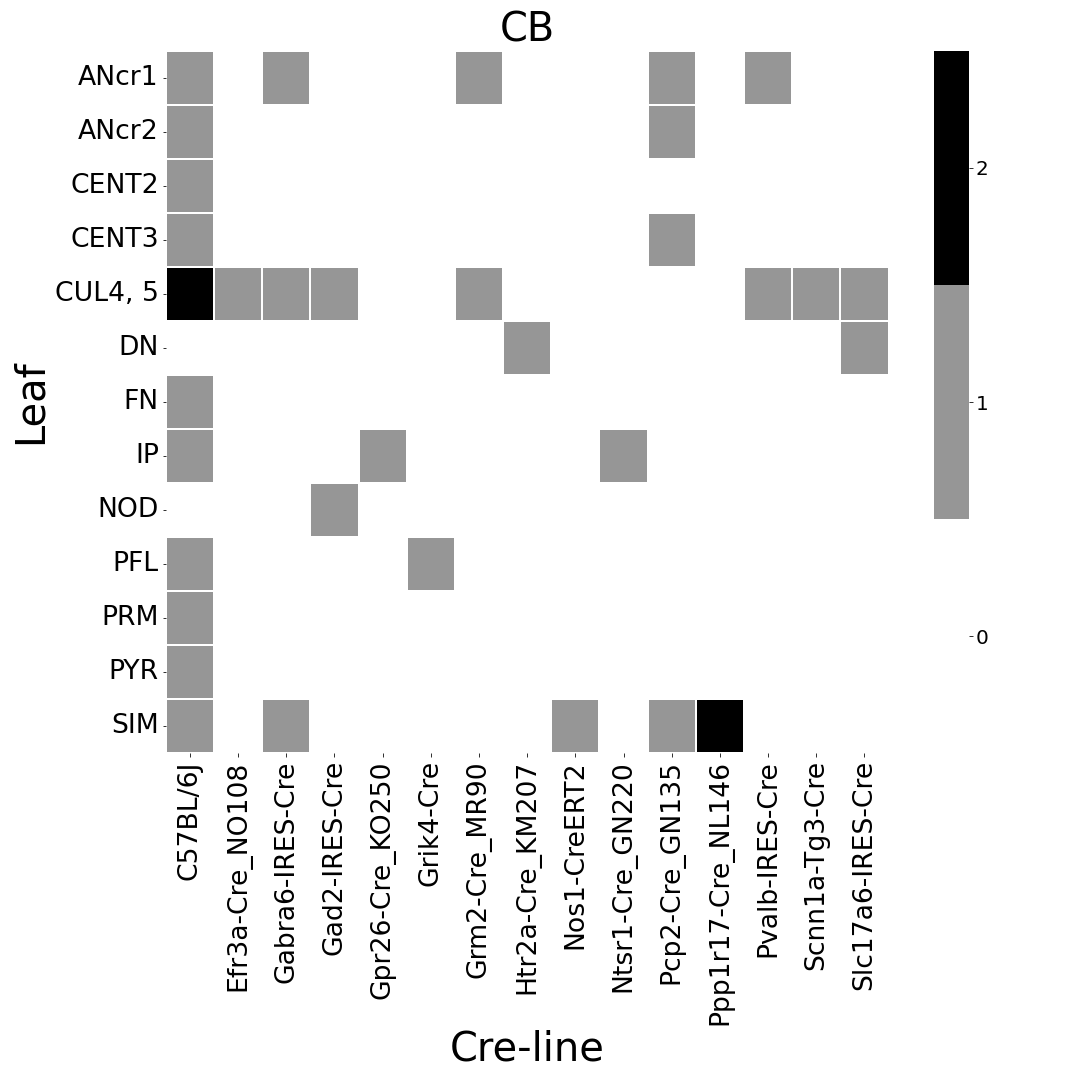
\includegraphics[width = 7in]{figs/CB centroid density.png}
        \caption{Abundances of cre-line and leaf-centroid combinations.}
            \label{fig:my_label}
\end{figure}
\newpage

\begin{figure}[H]
    \centering
    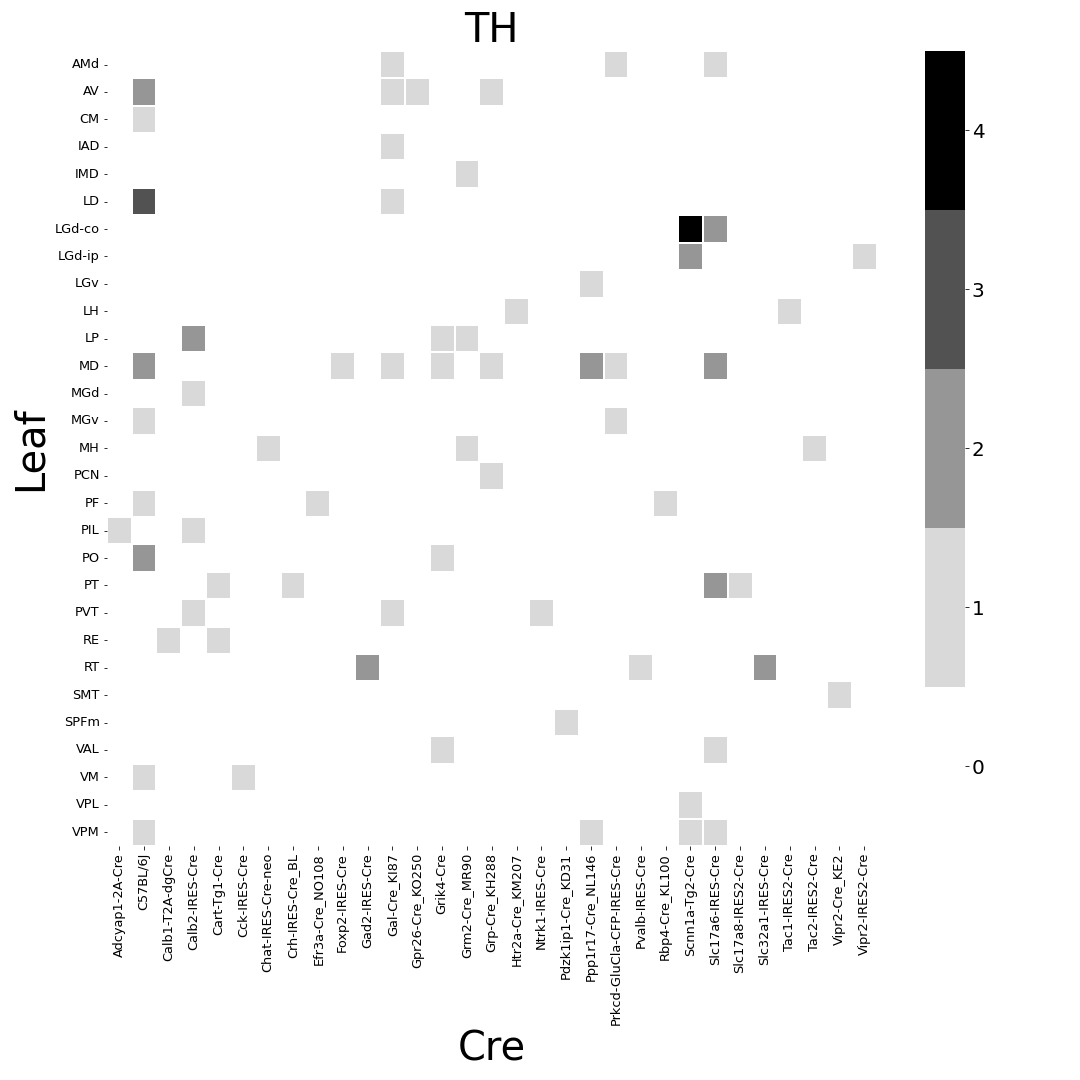
\includegraphics[width = 7in]{figs/TH centroid density.png}
    \caption{Abundances of cre-line and leaf-centroid combinations.}
    \label{fig:my_label}
\end{figure}
\newpage

\begin{figure}[H]
    \centering
    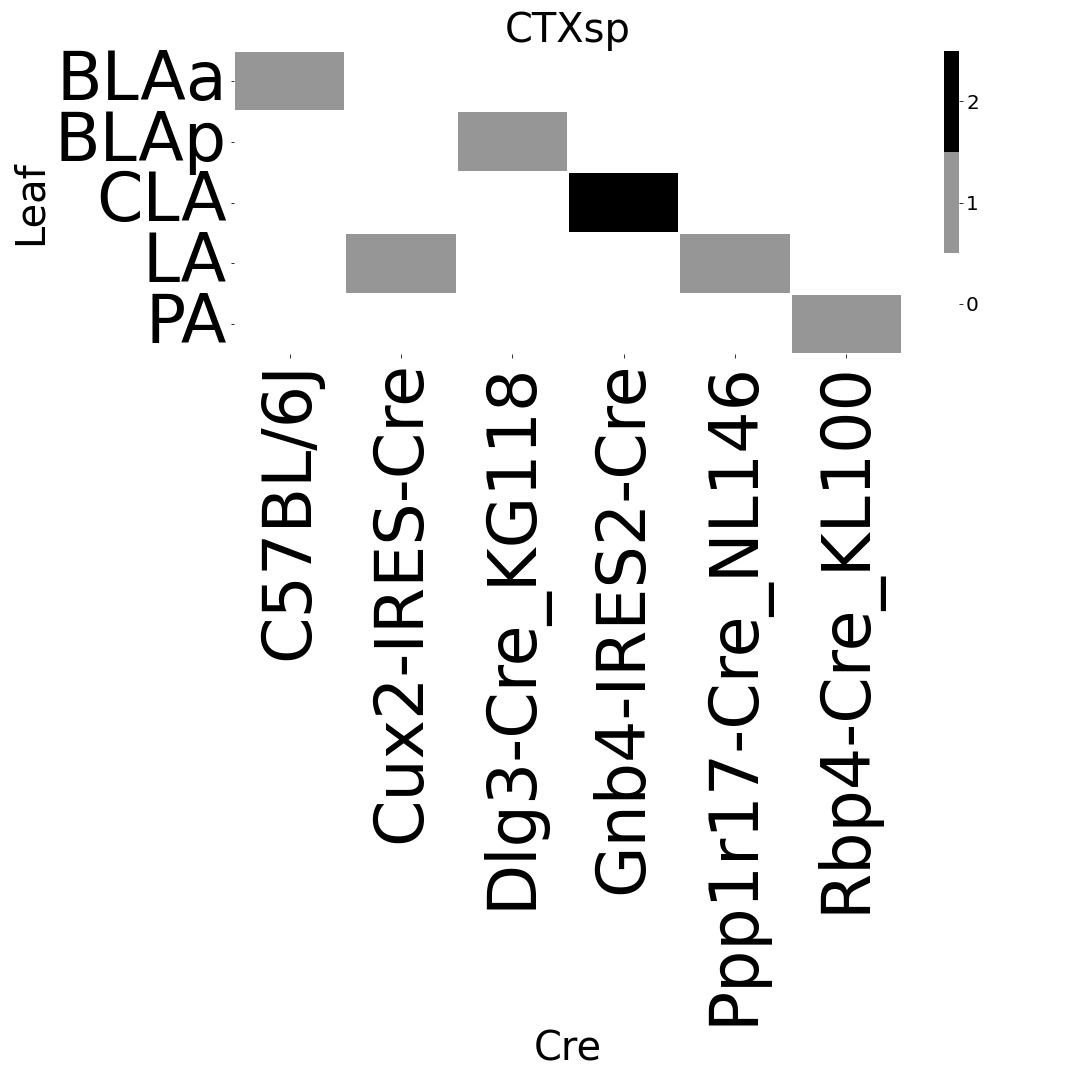
\includegraphics[width = 7in]{figs/CTXsp centroid density.png}
    \caption{Abundances of cre-line and leaf-centroid combinations.}
    \label{fig:my_label}
\end{figure}
\newpage

\begin{figure}[H]
    \centering
    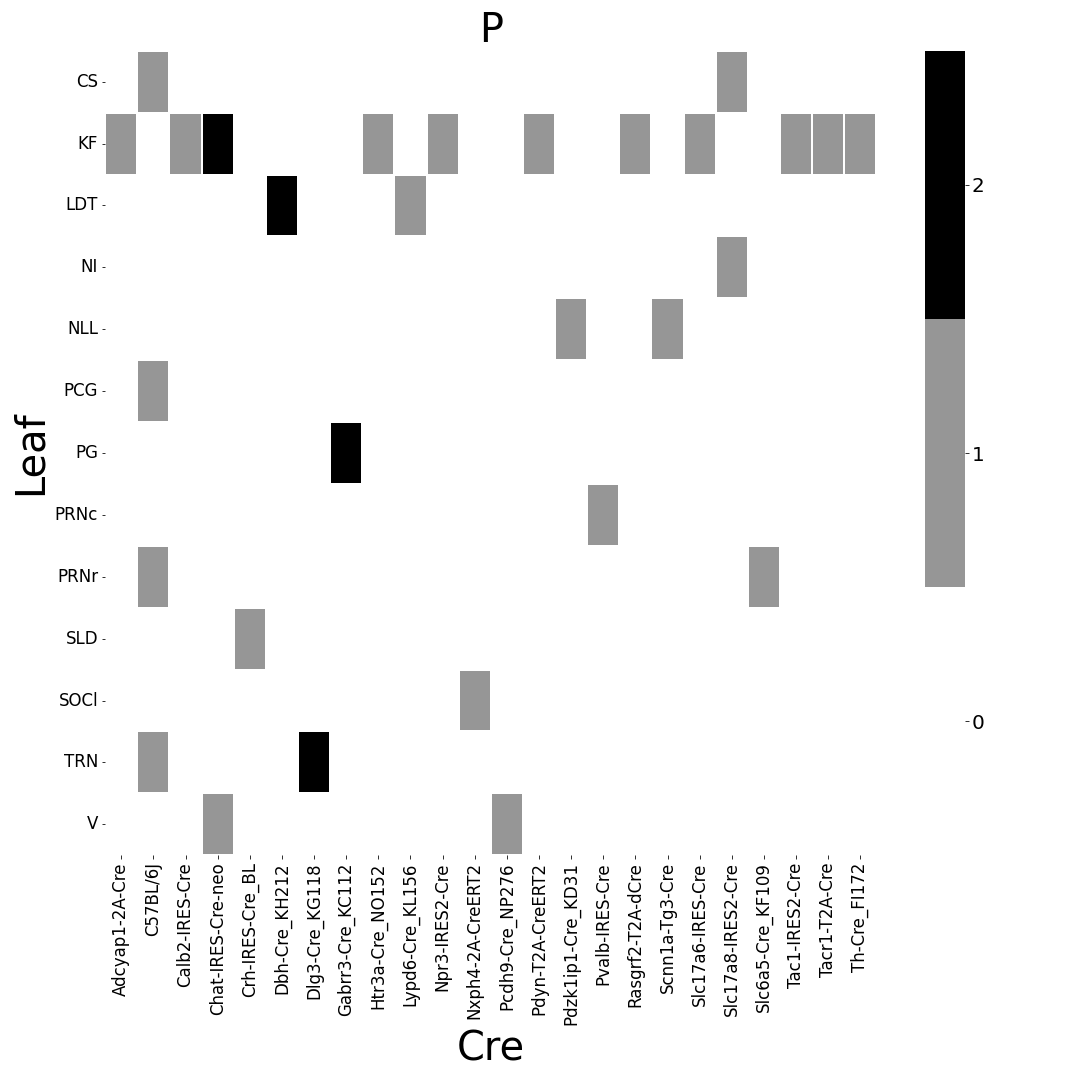
\includegraphics[width = 7in]{figs/P centroid density.png}
        \caption{Abundances of cre-line and leaf-centroid combinations.}
    \label{fig:my_label}
\end{figure}
\newpage

\begin{figure}[H]
    \centering
    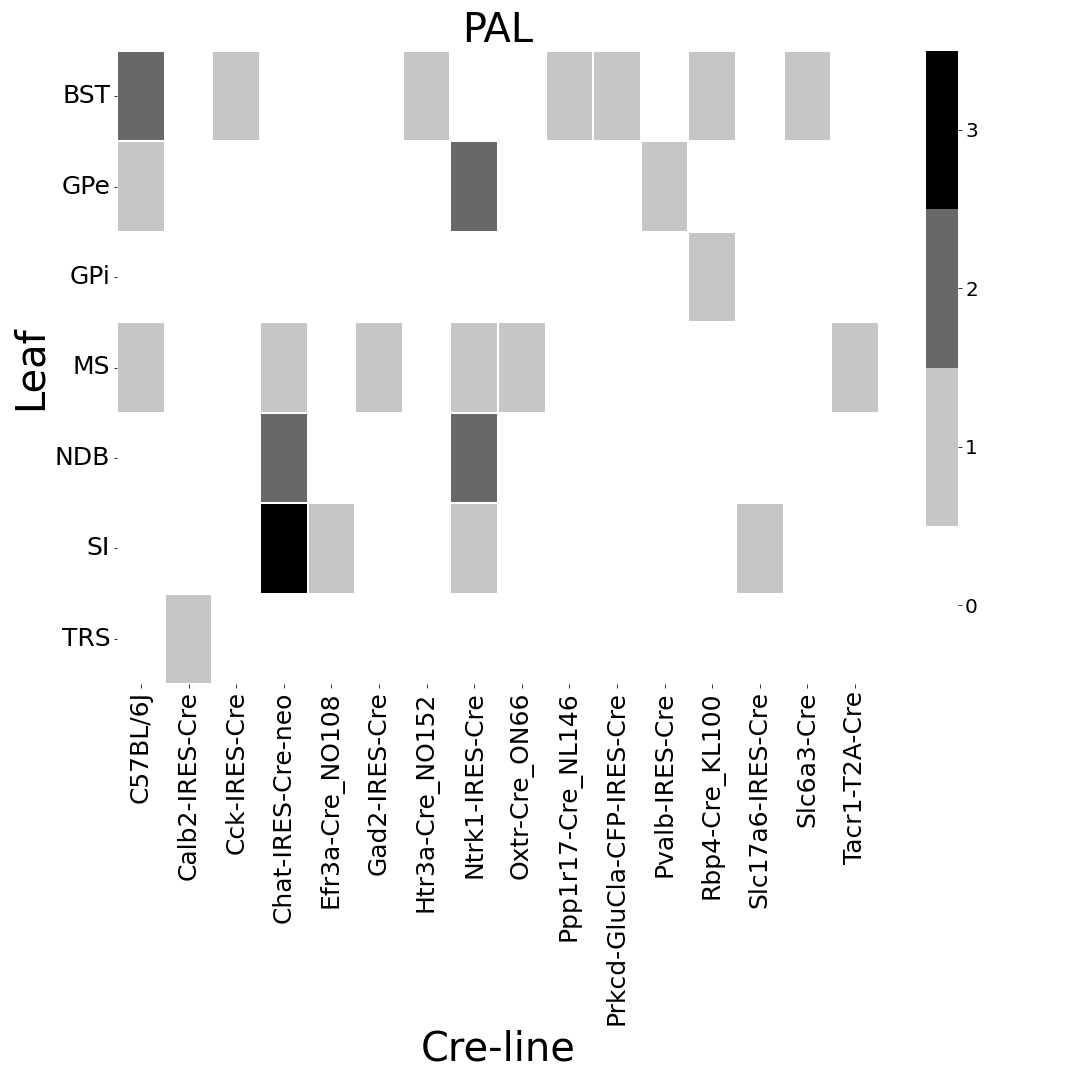
\includegraphics[width = 7in]{figs/PAL centroid density.png} 
        \caption{Abundances of cre-line and leaf-centroid combinations.}
    \label{fig:my_label}
\end{figure}
\newpage

\begin{figure}[H]
    \centering
    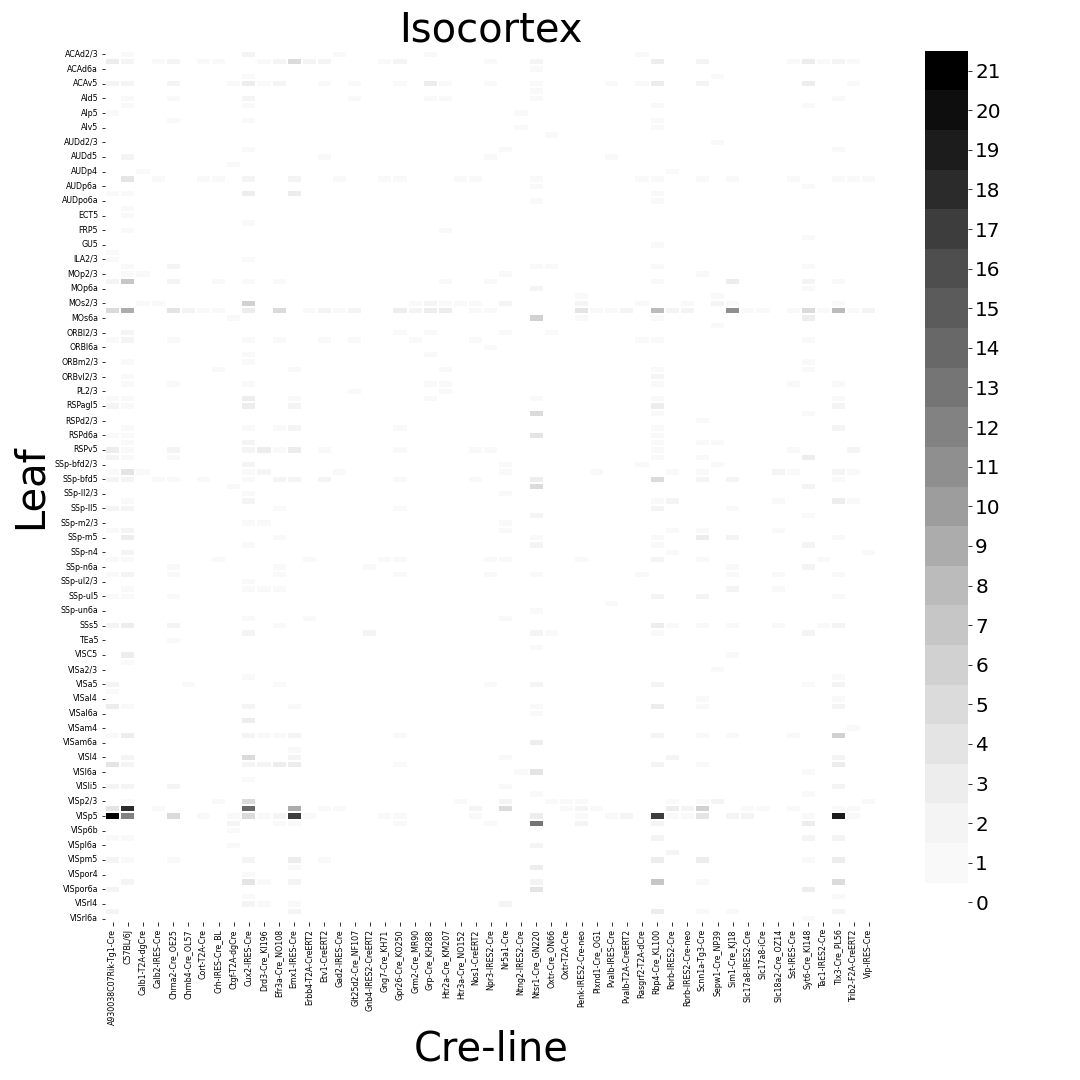
\includegraphics[width = 7in]{figs/Isocortex centroid density.png}
     \caption{Abundances of cre-line and leaf-centroid combinations.}
    \label{fig:iso_count}
\end{figure}
\newpage

\begin{figure}[H]
    \centering
    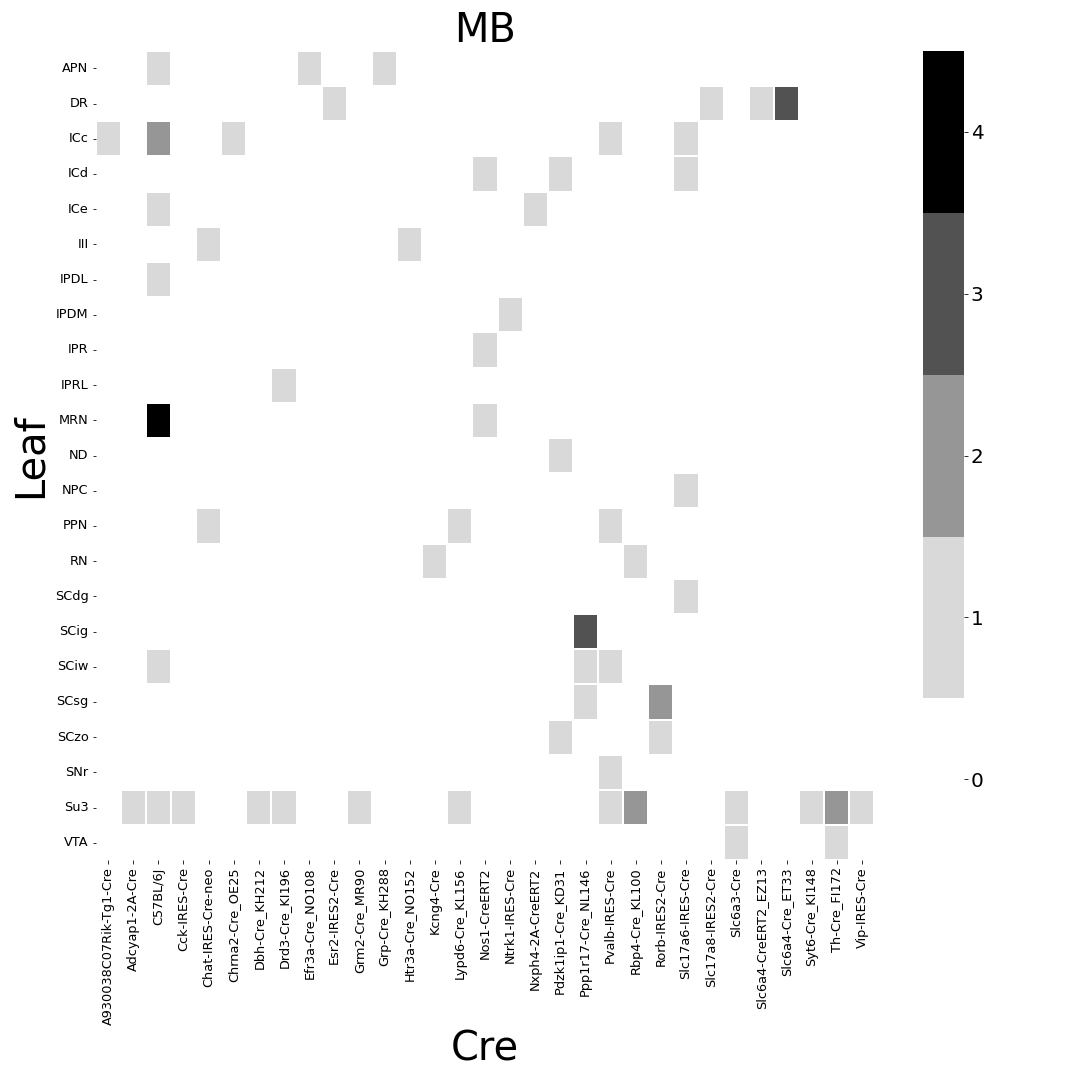
\includegraphics[width = 7in]{figs/MB centroid density.png} 
     \caption{Abundances of cre-line and leaf-centroid combinations.}
    \label{fig:my_label}
\end{figure}
\newpage

\begin{figure}[H]
    \centering
    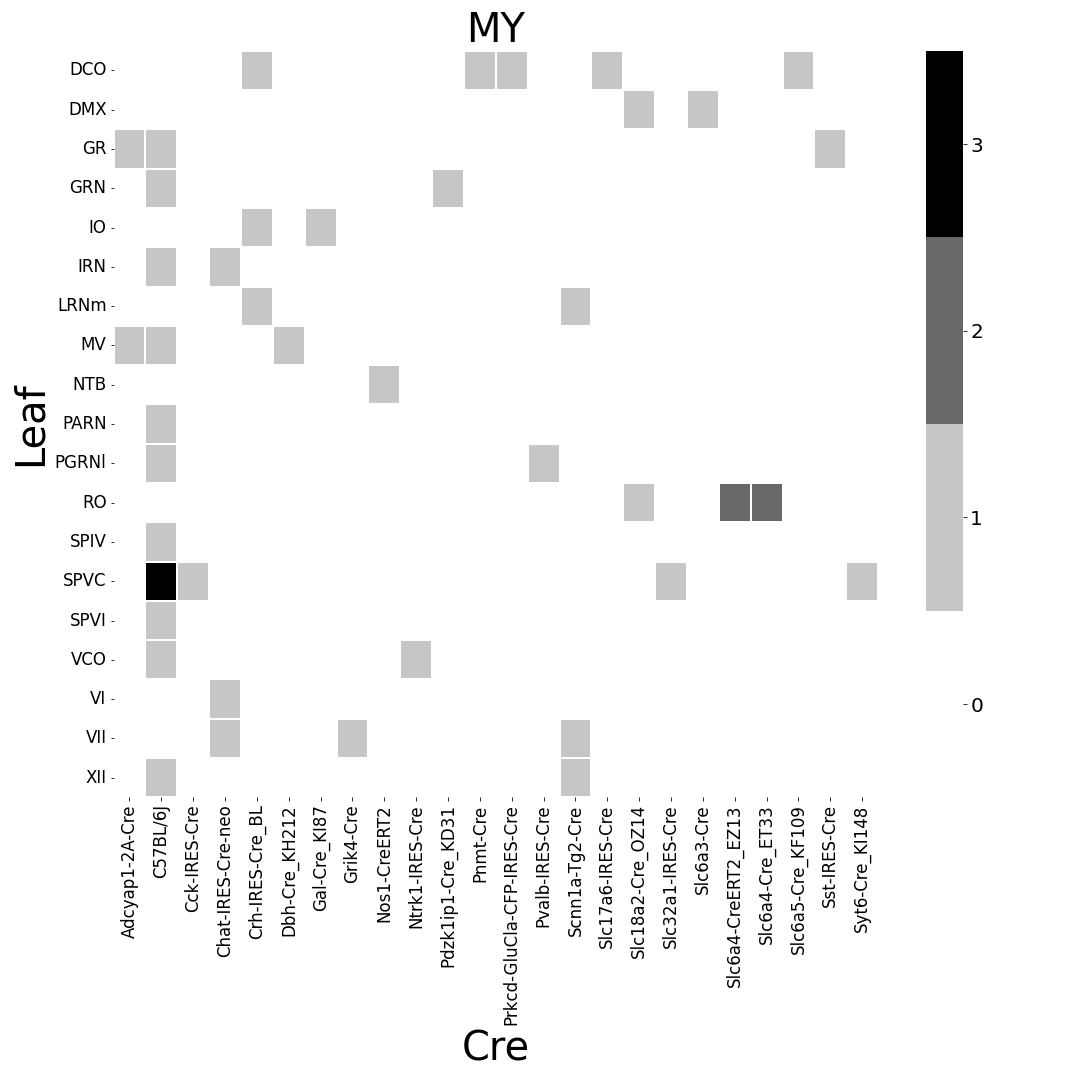
\includegraphics[width = 7in]{figs/MY centroid density.png} 
     \caption{Abundances of cre-line and leaf-centroid combinations.}
    \label{fig:my_label}
\end{figure}
\newpage

\begin{figure}[H]
    \centering
    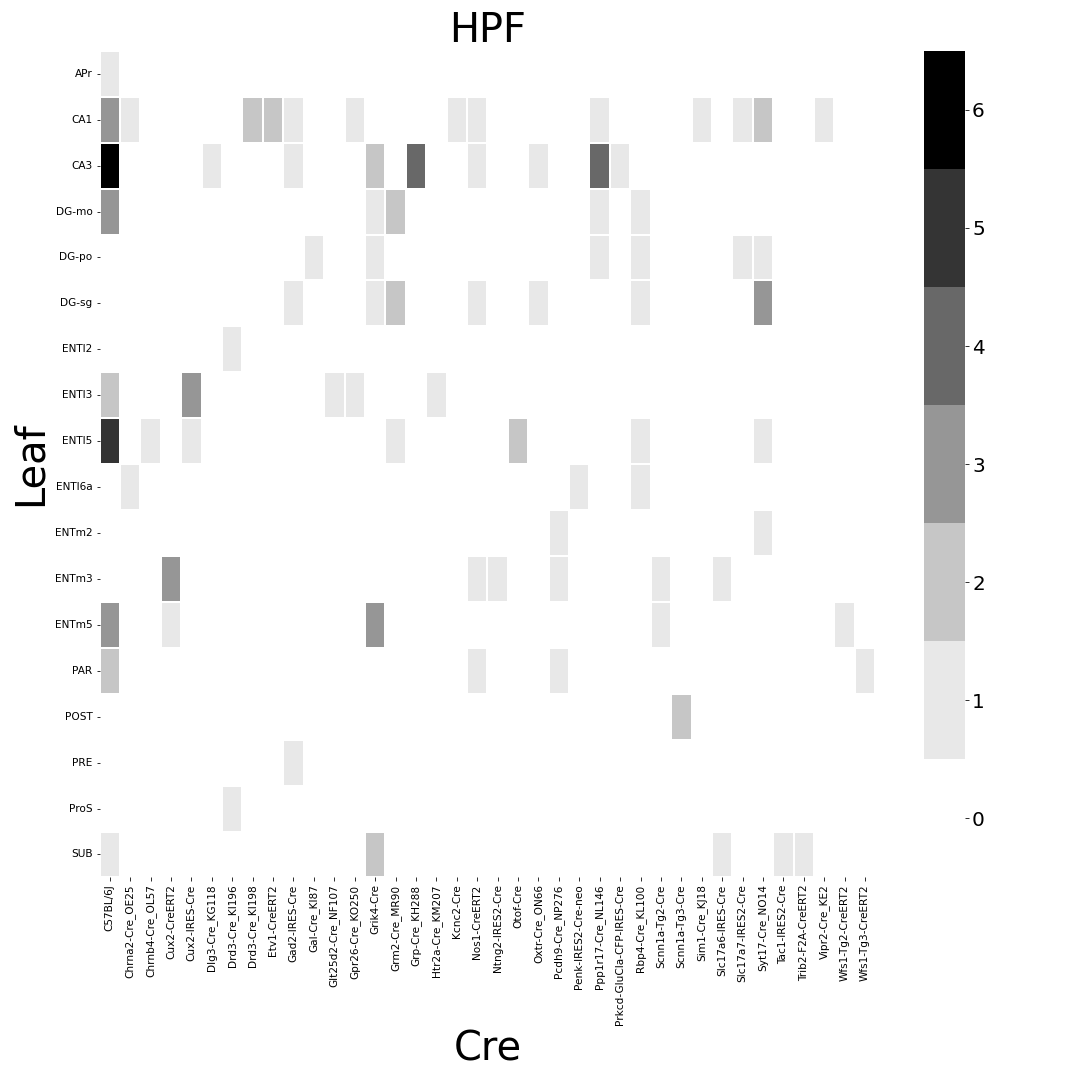
\includegraphics[width = 7in]{figs/HPF centroid density.png} 
     \caption{Abundances of cre-line and leaf-centroid combinations.}
    \label{fig:my_label}
\end{figure}
\newpage

\begin{figure}[H]
    \centering
    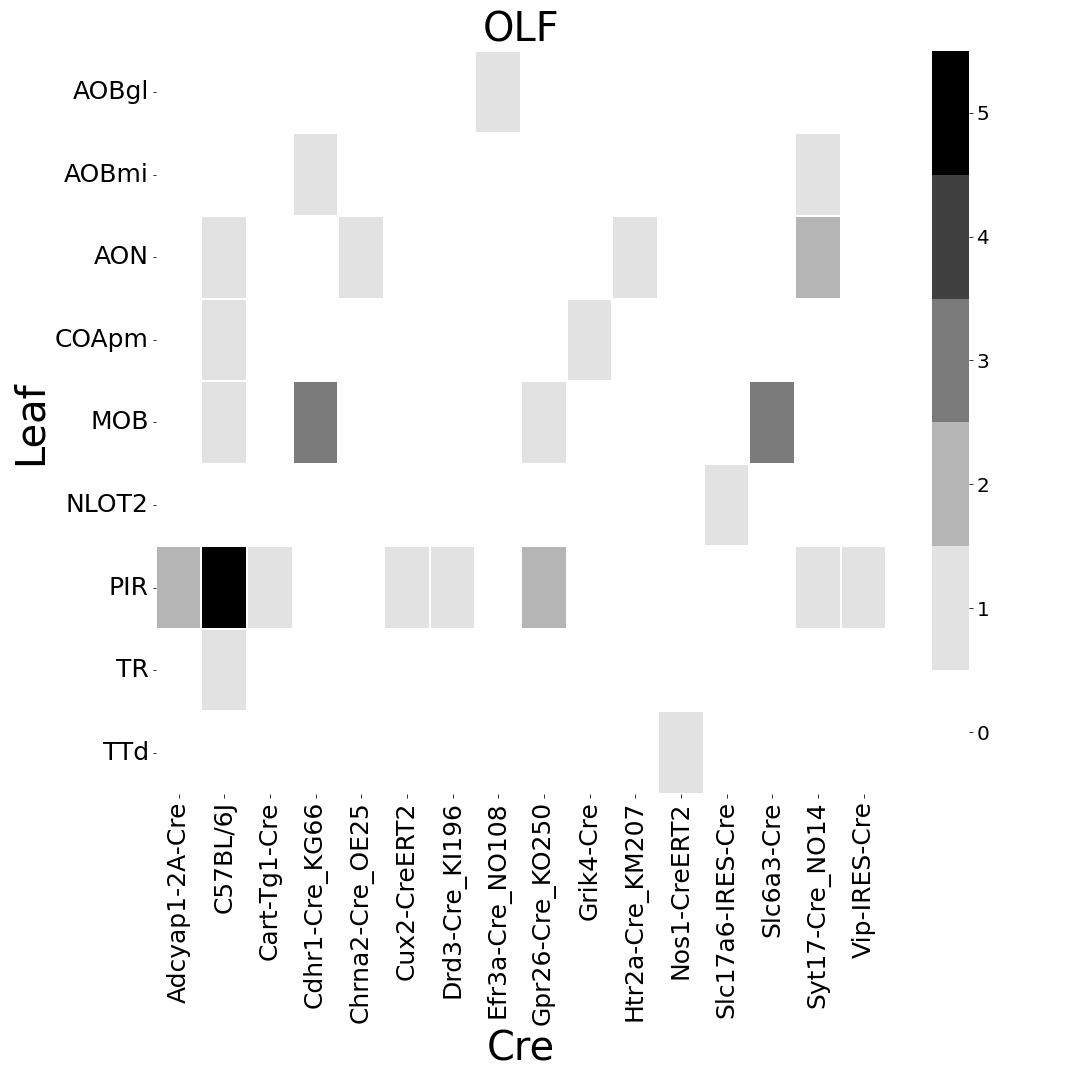
\includegraphics[width = 7in]{figs/OLF centroid density.png} 
     \caption{Abundances of cre-line and leaf-centroid combinations.}
    \label{fig:my_label}
\end{figure}
\newpage

\begin{figure}[H]
    \centering
    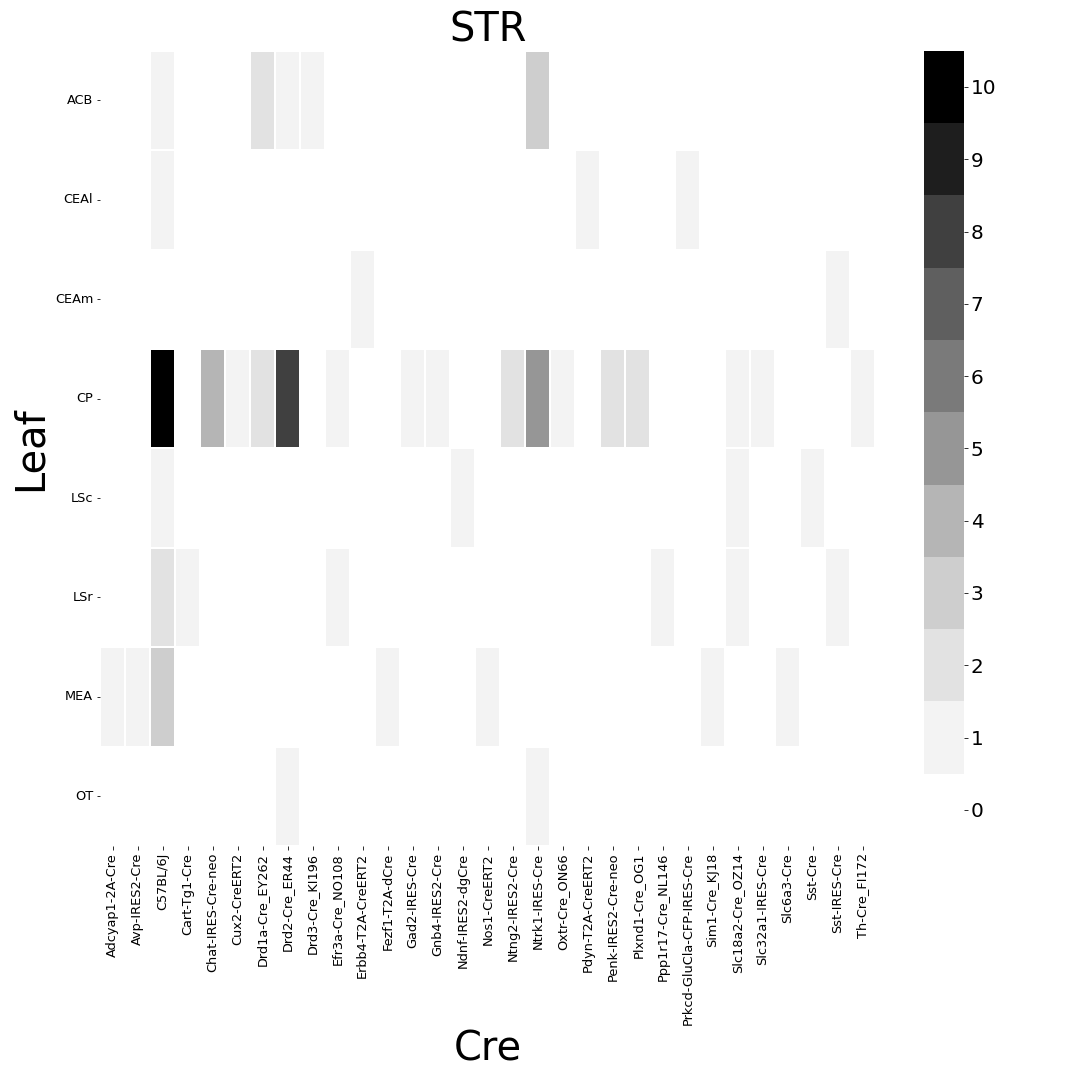
\includegraphics[width = 7in]{figs/STR centroid density.png} 
     \caption{Abundances of cre-line and leaf-centroid combinations.}
    \label{fig:my_label}
\end{figure}
\newpage

\begin{figure}[H]
    \centering
    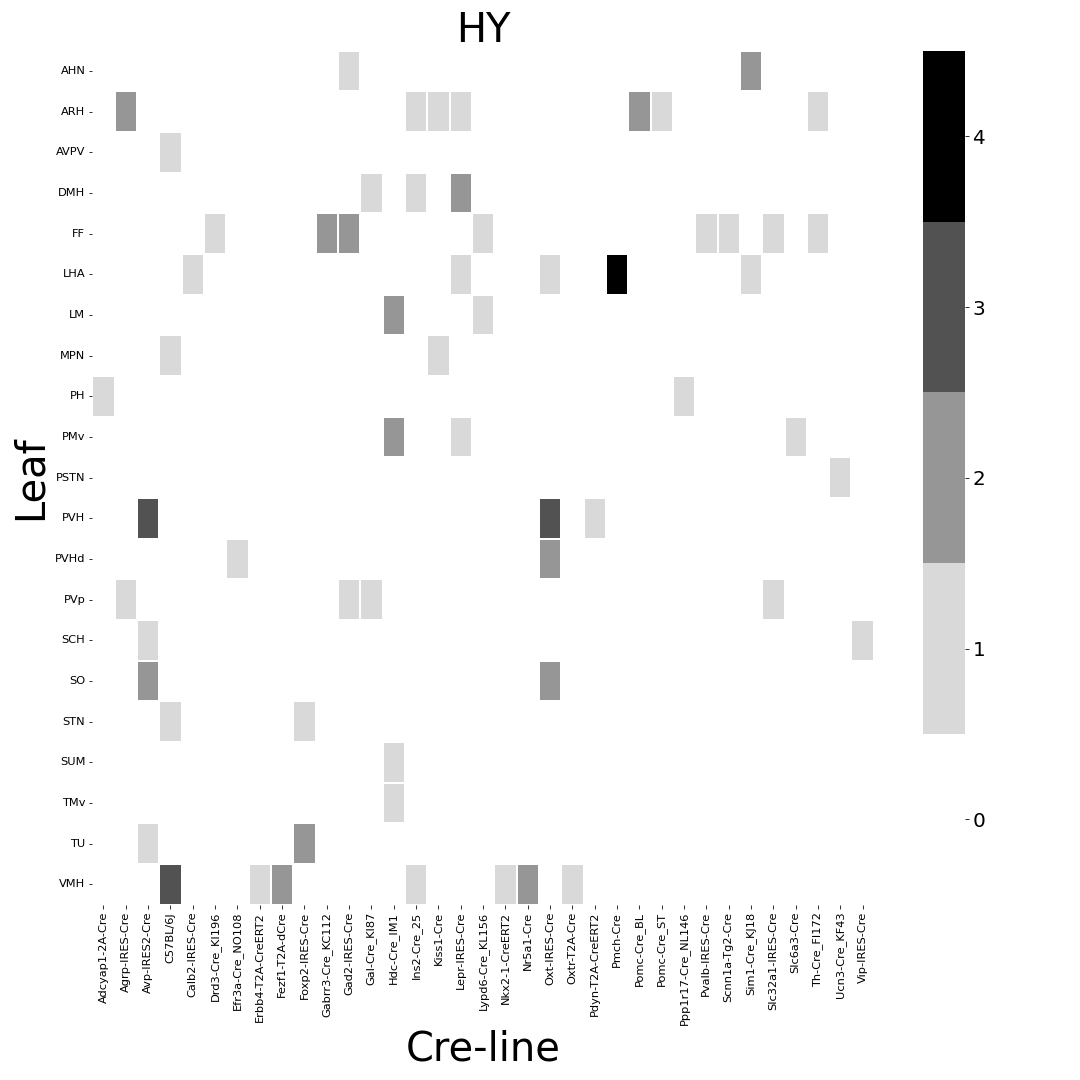
\includegraphics[width = 7in]{figs/HY centroid density.png} 
     \caption{Abundances of cre-line and leaf-centroid combinations.}
    \label{fig:my_label}
\end{figure}

\newpage

\subsection{Distances between structures}

\begin{figure}[H]
    \centering
    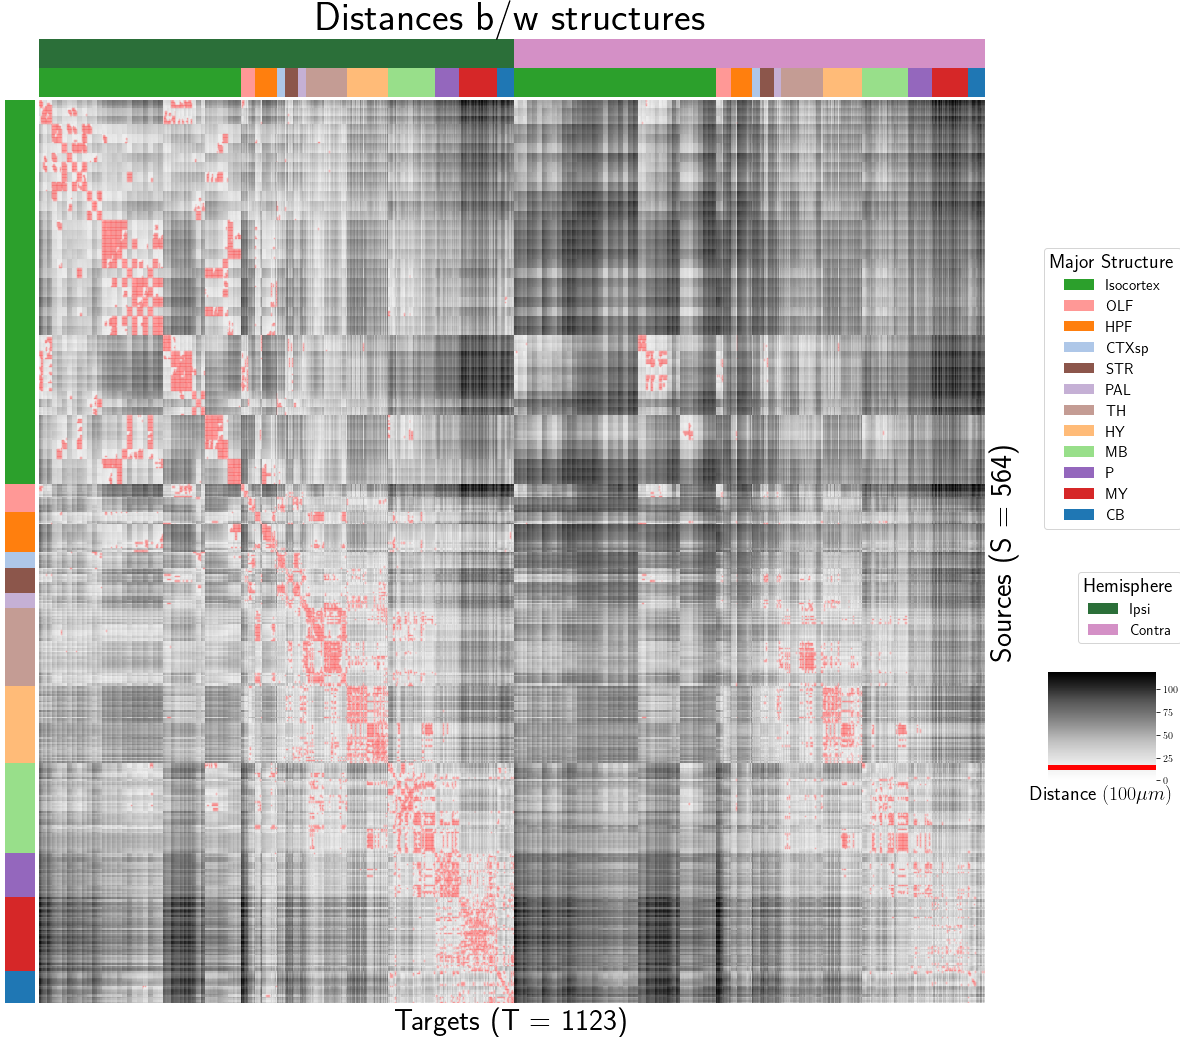
\includegraphics[width = 7in]{figs/distances_leafs.png} 
    \caption{Distance between structures.  Short-range connections are masked in red}
    \label{fig:dist_bw_str}
\end{figure}

\newpage

\subsection{Model evaluation}
\label{supp_sec:model-evaluation}

We give information on the quality of our models.
This includes the sizes of our evaluation sets in leave-one-out cross-validation and additional losses in the injection-normalized case.


\paragraph{Number of experiments in evaluation sets}

In order to compare between methods, we therefore restrict to the smallest set of evaluation indices, which is to say, virus-leaf combinations that are present at least twice. 
This means that our evaluation set in size is smaller than our evaluation set is smaller in size than our overall list of experiments.


\begin{table}[H]
\small
\begin{tabular}{lrrr}
\toprule
{} &  Total &  Cre-Leaf & Cre-leaf over threshold \\
\midrule
Isocortex &     36 &         4  & 4\\
OLF       &      7 &         2 & 2\\
HPF       &    122 &        62 & 59\\
CTXsp     &     85 &        41 & 38\\
STR       &   1128 &       732& 7 \\
PAL       &     68 &        18 & 17\\
TH        &     46 &         7& 7 \\
HY        &     35 &        17& 17 \\
MB        &     33 &         8 & 8\\
P         &     30 &        11& 11\\
MY        &     78 &        45 & 44\\
CB        &     83 &        29& 29 \\
\bottomrule
\end{tabular}
\caption{Number of experiments available to evaluate models in leave-one-out cross validation. 
Models that rely on a finer granularity of modeling have less data available to validate with.} 
\label{tab:eval_size}
\end{table}

\newpage

\paragraph{Injection-normalized losses}
To compare with the injection-normalization procedure from \citet{Knox2019-ot}, we also remove experiments with small injection, and here give results for this slightly reduced set using injection-normalization.
That is, instead of dividing the projection signal of each experiment by its $l1$ norm, we divide by the $l1$ norm of the corresponding injection signal.
We find that setting a summed injection-signal of threshold of $1$ is sufficient for evading pathological edge cases in this normalization, while still retaining a large evaluation set.

\begin{table}[H]
\begin{tabular}{lrrrrrrr}
\toprule
$\widehat f$ &           Mean & \multicolumn{5}{l}{NW} &     EL \\
$\mathcal D$ & $I_c \cap I_L$ & $I_c \cap I_M$ & $I_c \cap I_L$ &  $I_L$ & $I_{wt} \cap I_M$ &  $I_M$ &  $I_L$ \\
\midrule
Isocortex &          0.413 &          0.453 &          0.408 &  0.538 &             0.528 &  0.528 &  \textbf{0.396} \\
OLF       &          0.499 &          0.504 &          0.494 &  0.441 &             0.543 &  0.543 &  \textbf{0.437} \\
HPF       &          0.336 &          0.483 &          0.332 &  0.444 &             0.501 &  0.501 & \textbf{ 0.321} \\
CTXsp     &          0.497 &          0.497 &          0.497 &  0.497 &             0.497 &  0.497 &  0.497 \\
STR       &          0.359 &          0.386 &          0.359 &  0.364 &             0.433 &  0.433 &\textbf{  0.322} \\
PAL       &          0.519 &          0.497 &          0.519 &  0.436 &             0.459 &  0.459 &\textbf{  0.434} \\
TH        &          0.769 &          0.767 &          0.769 &  \textbf{0.514} &             0.539 &  0.539 &  0.556 \\
HY        &          0.414 &          0.439 &          0.414 &  0.441 &             0.452 &  0.452 & \textbf{ 0.399} \\
MB        &          0.459 &          0.396 &          0.397 &  0.358 &         \textbf{    0.324 }& \textbf{ 0.324 }&  0.403 \\
P         &          \textbf{0.562 }&    \textbf{     0.562 }&      \textbf{    0.562 }&  0.758 &             0.764 &  0.764 &  \textbf{0.562} \\
MY        &          0.699 &          0.552 &          0.621 &  \textbf{0.439 }&             0.578 &  0.578 & \textbf{ 0.439} \\
CB        &          0.849 &          0.689 &          0.849 &  0.500 &             0.615 &  0.615 & \textbf{ 0.495} \\
\bottomrule
\end{tabular}
\caption{Losses from leave-one-out cross-validation of candidate for injection-normalized structural connectivity on injection-thresholded evaluation set. \textbf{Bold} numbers are best for their major structure.} 
\label{tab:eval_size}
\end{table}

\newpage
\paragraph{Projection-normalized losses on thresholded set}

We also give results for the projection-normalization procedure from the main text on this reduced subset.

\begin{table}[H]
\begin{tabular}{lrrrrrrr}
\toprule
$\widehat f$ &           Mean & \multicolumn{5}{l}{NW} &     EL \\
$\mathcal D$ & $I_c \cap I_L$ & $I_c \cap I_M$ & $I_c \cap I_L$ &  $I_L$ & $I_{wt} \cap I_M$ &  $I_M$ &  $I_L$ \\
\midrule
Isocortex &          0.229 &          0.248 &          0.224 &  0.274 &             0.269 &  0.269 &  \textbf{0.217} \\
OLF       &          0.193 &          0.233 &          0.191 &   \textbf{0.135} &             0.179 &  0.179 &  0.138 \\
HPF       &          0.178 &          0.342 &          \textbf{ 0.172 }&  0.212 &             0.235 &  0.235 &   \textbf{0.172} \\
CTXsp     &          \textbf{ 0.621 }&      \textbf{     0.621 }&       \textbf{    0.621} &   \textbf{0.621 }&            \textbf{  0.621} &   \textbf{0.621 }&   \textbf{0.621 }\\
STR       &          0.128 &         \textbf{  0.117} &          0.124 &  0.171 &             0.234 &  0.234 &  0.125 \\
PAL       &          0.203 &          0.205 &          0.203 &  0.295 &             0.291 &  0.291 & \textbf{  0.188 }\\
TH        &          0.673 &          0.664 &          0.673 &   \textbf{0.358} &             0.379 &  0.379 &  0.417 \\
HY        &          0.358 &          0.378 &          0.351 &  0.331 &             0.312 &   \textbf{0.312} &  0.314 \\
MB        &          0.168 &          0.191 &         \textbf{ 0.160 }&  0.199 &             0.202 &  0.202 & \textbf{ 0.160} \\
P         &          0.292 &          0.292 &          0.292 &  0.299 &             0.299 &  0.299 &\textbf{  0.287 }\\
MY        &          0.268 &          0.347 &          0.268 &  \textbf{0.167} &             0.189 &  0.189 &  0.196 \\
CB        &          0.062 &          0.062 &          0.062 &  0.068 &             0.108 &  0.108 &  \textbf{0.061 }\\
\bottomrule
\end{tabular}
\caption{Losses from leave-one-out cross-validation of candidate for normalized structural connectivity on injection-thresholded evaluation set. \textbf{Bold} numbers are best for their major structure.}
\label{tab:crossvalidation}
\end{table}



\newpage 
\section{Supplemental methods}
\label{supp_sec:methods}

This section consists of additional information on preprocessing of the neural connectivity data, estimation of connectivity, and matrix factorization.

\subsection{Data preprocessing}
\label{supp_sec:dp}

Several data prepreprocessing steps take place prior to evaluations of the connectivity matrices.
These steps are described in Algorithm \pre.
The arguments of this normalization process - injection signals $x(i)$, projection signals $y(i)$, injection fraction $F(i)$, and data quality mask $q(i)$ - were downloaded using the Allen SDK. %and injection fraction $F(i)$ 
The injections and projection signals $ \mathcal B \to \mathbb [0,1]$ were segmented manually in histological analysis.
The projection signal gives the proportion of pixels within the voxel displaying fluorescence, and the injection signal gives the proportion of pixels within the histologically-selected injection subset displaying fluorescence.
The injection fraction $ \mathcal B \to \mathbb [0,1]$ gives the proportion of pixels within each voxel in the injection subset.
Finally, the data quality mask $ \mathcal B \to \mathbb \{0,1\}$ gives the voxels that have valid data.

%We also have a map $A: \mathbb R \to \mathbb R^{|S|}$ where $S$ is the number of structures that takes the average value for voxels in that structure
Our preprocessing makes use of the above ingredients, as well as several other essential steps.
First, we compute the weighted injection centroid
\begin{eqnarray*}
c(i) &= \sum_{l \in \mathcal B} x(i)(l) l
\end{eqnarray*}
where $x(i)(l)$ is the injection density at location $l \in \mathbb R^3$.
Given a regionalization $\mathcal R$ from the Allen SDK, we can also access regionalization map $R: \mathcal B  \to \mathcal R $.
This induces a functional of connectivities from the space of maps $\{\mathcal X = x: \mathcal B \to [0,1]$
\begin{eqnarray*}
1_{\mathcal R}: \mathcal X &\to \mathcal R \times \mathbb R_{\geq 0} \\
x &\mapsto \sum_{l \in r}  x(l)  \text{ for } r \in \mathcal R.
\end{eqnarray*}
%This map depends on the choice of regionalization; we regionalize at the leaf level.
We also can restrict a signal to a individual structure as
\begin{eqnarray*}
1 |_s :  \mathcal X &\to  \mathcal X \\
 x(l) &= \begin{cases} 
 x(l) \text{ if } l \in S \\
 0 \text{ otherwise }.
 \end{cases}
\end{eqnarray*}
Finally, given a vector or array $a \in \mathbb R^T$, we have the $L1$ normalization map
\begin{eqnarray*}
n: a &\mapsto \frac{a}{\sum_{j = 1}^T a_j}.
\end{eqnarray*}

We define these objects as functions and functionals, but this is for notational convenience and non-essential.
A function $x(i):\mathcal B \to [0,1]$ is mathematically equivalent to the graph $\mathcal G(x(i)) \in \mathcal B \times [0,1]$.
As an abuse of notation, we define $x \odot x' := z$ such that $z(l) = x(l) x'(l)$ for all $l \in \mathcal B$.
Also, denote $m(i)$ as the major structure containing experiment $i$.
We then can write the preprocessing algorithm.

\begin{algorithm}[H]
\floatname{algorithm}{\pre}%{\preprocess}
\caption{{\bf Input} Injection $x(i)$, Projection $y(i)$, Injection centroid $c(i) \in \mathbb R^3$, injection fraction $F(i)$, data quality mask $q(i)$}
\label{alg:preprocess}
\begin{algorithmic}
\State Injection fraction $x_F(i) \gets x(i) \odot F(i)$
\State Data-quality censor $y_q (i) \gets  \odot y(i) \odot q(i) , x_q(i) \gets x_F(i) \odot q(i)$
\State Restrict injection $x_m(i) = 1 |_{m(i)} x_q(i) $.
\State Compute centroid $c(i)$ from $x_m(i) $
\State Regionalize $\tilde y_{\mathcal T} (i) \gets 1_{\mathcal T}(  y_q(i))$
\State Normalize $ y_{\mathcal T} (i) \gets n(\tilde y_{\mathcal T} (i) )$
 \State {\bf Output}$\tilde y_{\mathcal T} (i) $, $c(i)$ 
\end{algorithmic}
\end{algorithm}


%The data-quality censor is established by \skcomment{fill}
%We find the $l2$ norm not appropriate in a few ways 1) there is not a clear inner product structure on the connectome.
%doesn't matter if we normalize prior to regionalization as long as we don't correct for density of the target region.
%which, due to normalization, can be rewritten as simply the $l2$ loss $\|y - \hat y\|.$  Note that, due to normalization, $\|y - \hat y\| = \langle y - \hat y , y - \hat y \rangle = 2 - 2 \langle y, \hat y\rangle $, and, applying normalization again, $ \langle y, \hat y\rangle $ is the vector cosine of $\hat y$ and $y$.

\newpage
\subsection{Estimators}
\label{supp_sec:estimators}
As mentioned previously, we can consider our estimators as modeling a connectivity vector $f_{\mathcal T} (v,s)  \in \mathbb R_{\geq 0}^T$.
Thus, for the remainder of this section, we will discuss only $f (v,s)$.
We review the Nadaraya-Watson estimator from  \citet{Knox2019-ot}, and describe its conversion into our cell-class specific Expected Loss estimator.

\subsubsection{Centroid-based Nadaraya-Watson}

In the Nadaraya-Watson approach of \citet{Knox2019-ot}, the injection is considered only through its centroid $c(i)$, and the projection is considered regionalized.
%The prediction for a given region is then given by the integral of predictions over that region, which is computed as a sum over voxels.
That is,
\begin{eqnarray*}
f_*(i) = \{c(i), y_{\mathcal T}(i)\}.
\end{eqnarray*}
Since the injection is considered only by its centroid, this model only generates predictions for particular locations $l$, and the prediction for a structure $s$ is given by integrating over locations within the structure
\begin{eqnarray*}
\label{eq:regionalize}
f^* (\hat f (f_*(\mathcal D))) (v,s) = \sum_{l \in s} \hat f (f_*(\mathcal D(I))) (v,l ).
\end{eqnarray*}
Here, $I$ is the training data, and $\hat f$ is the Nadaraya-Watson estimator
\begin{eqnarray*}
\hat f_{NW}( c(I) , y_{\mathcal T}(I) ) (l) :=  \sum_{i \in I} \frac{ \omega_{i l}}{\sum_{i \in I} \omega_{i l}} y_{\mathcal T}(i)
\end{eqnarray*}
where $\omega_{i l } := \exp( - \gamma d( l , c(i))^2 )$ and $d$ is the Euclidean distance between centroid $c(i)$ and voxel with position $l$.

Several facets of the estimator are visible here. %$f_{NW}^{\gamma}$ is the Nadaraya-Watson estimator with smoothing given by inverse-bandwidth $\gamma$.
A smaller $\gamma$ corresponds to a greater amount of smoothing, and the index set $I \subseteq  \{1:n\}$ generally depends on $s$ and $v$.
Fitting $\gamma$ via empirical risk minimization therefore bridges between $1$-nearest neighbor prediction and averaging of all experiments in $I$.
In \citet{Knox2019-ot}, $I$ consisted of experiments sharing the same brain division, i.e. $I = I_m$, while restricting of index set to only include experiments with the same cell class gives the class-specific Cre-NW model.
Despite this restriction, we fit $\gamma$ for each $m$ rather than a smaller subset like $s$ or $v$.
That is,
\begin{eqnarray}
\label{eq:gamma_sel}
\widehat \gamma_m =  \arg \min_{\gamma \in \mathbb R_{\geq 0}} \frac{1}{|\{s,v\}|} \sum_{s,v \in \{m,\mathcal V\}} \frac{1}{ |I_{s} \cap I_v |} \sum_{i \in (I_{s} \cap I_v ) } \ell (y_{\mathcal T}(i)), \hat f_{\mathcal T} (f_*(\mathcal D(v,s) \setminus i)) .
\end{eqnarray}

\newpage
\subsubsection{The Expected-Loss estimator}

\label{supp_sec:el}

Besides the injection location, the targeted cell class also influences projection.
Since Cre-lines that target similar classes are induce similar projections, and including similar Cre-lines in the Nadaraya-Watson estimator increases effective sample size, we introduce an estimator that assigns a predictive weight to each training point that depends both on its centroid-distance and Cre-line.
This weight is determined by the expected prediction error of each of the two feature types, as determined by cross-validation.
For this reason, we call this the Expected Loss Estimator.
The resulting weights are then utilized in a Nadaraya-Watson estimator in a final prediction step.
%It shares thefine-scale spatial resolution with \citet{Knox2019-ot}, but in addition enables us to model a particular cell-class $v$.

We formalize Cre-line behavior as the average regionalized projection of a Cre-line in a given structure (i.e. leaf).
This vectorization of categorical information is known as \textbf{target encoding}, and we define this as $\bar y_{\mathcal T,s,v} := \frac{1}{|I_s \cap I_v|}  \sum_{i \in (I_s \cap I_v)} y_{\mathcal T}(i)$.
We define a \textbf{Cre-distance} in a leaf to be the distance between the target-encoded projections of two Cre-lines.
The relative predictive accuracy of Cre-distance and centroid distance is determined by fitting a surface of projection distance as a function of Cre-distance and centroid distance. 

In mathematical terms, our full feature set consists of the centroid coordinates and the target-encoded means of the combinations of virus type and injection-centroid structure.
That is, 
\begin{eqnarray*}
f_*({\mathcal D}_i) = \{c(i) , \{\bar y_{\mathcal T,s,v}  \forall v \}, y_{\mathcal T}(i) \}.
\end{eqnarray*}
$f^*$ is defined as in \eqref{eq:regionalize}.
The expected loss estimator is then 
\begin{eqnarray*}
\hat f_{EL} ( c(I),y_{\mathcal T} (I))(l,v) :=  \sum_{i \in I} \frac{ \nu_{ilv} }{\sum_{i \in I}  \nu_{ilv}  } y_{\mathcal T}(i)
\end{eqnarray*}
where
\begin{eqnarray*}
\nu_{ilv} := \exp (- \gamma g( d(l, c(i))^2, d(\bar y_{\mathcal T,s,v} , \bar y_{\mathcal T,s,v(i)}  )^2))
\end{eqnarray*}
and $s$ is the structure containing $l$.

The key step therefore is finding a suitable $g$ with which to weight the positional and Cre information.
Note that $g$ must be a concave, non-decreasing function of its arguments with with $g(0,0) = 0$, then $g$ defines a metric on the product of the metric spaces defined by experiment centroid and target-encoded cre-line, and $\hat f_{EL}$ is a Nadaraya-Watson estimator. 
A derivation of this fact is given later in this section, and we therefore use shape-constrained B-splines to estimate $g$.
Similarly to the Nadaraya-Watson model, we make the decision to fit a $g$ separately for each major brain division.
We can then select $\hat \gamma$ as in \ref{eq:gamma_sel}.

\newpage

\begin{figure}[H]
\begin{tabular}[t]{cc}
\subfloat[]{
    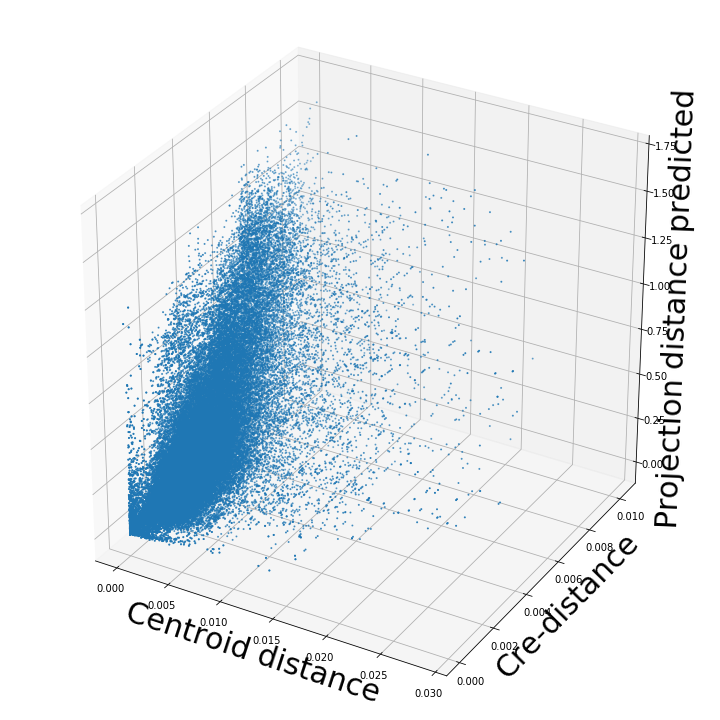
\includegraphics[width = 2.1in]{figs/315_summary_scatter.png}
   % \caption{Isocortex loss distribution}
    \label{fig:expected_loss} 
   }
    &
    \subfloat[]{
    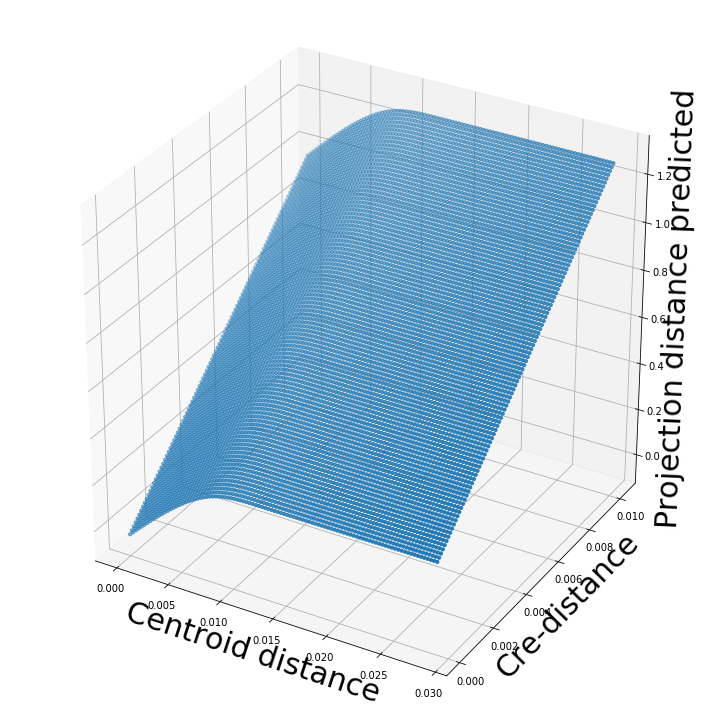
\includegraphics[width = 2.1in]{figs/315_summary_surface.png}
   % \caption{$\hat g$ fit to expected-loss using shape-constrained splines}
   \label{fig:expected_loss_surface}
    }
   \end{tabular}
   \caption{Fitting $g$.
   \ref{fig:expected_loss} Distribution of projection errors against centroid distance and cre-distance in Isocortex.
    \ref{fig:expected_loss_surface} $\hat g$ found using B-splines.
    }
   \end{figure}
   
  \newpage
  
%This contrasts with the models in \citet{Knox2019-ot} and \citet{Oh2014-kh}, where connectivity was directly estimated by $\hat f$ a function of $S$ without an integral.
%Since we wish to weight similar points more highly, we weight distances in cre-space and centroid-space by how well they predict the response variable.
%Due to the fact that the cre-space is defined with respect to the response variable, points are removed from their cre-mean prior to cross-validation.
%Figure shows an example of such an estimated $g$.

%In the low-sample size setting, it is worth utilizing points from similar groups.

%\newpage

%\begin{algorithmic}
%\label{alg:model}
%\begin{algorithm}{Injection centroids $c(1:n)$, normalized projections $n(r(y(1:n)))$, viruses $v(1:n)$. target centroid $c$, target virus $v$}
%\STATE Get structures $s(1:n) = r(c(1:n))$, $s = r(c)$
%\STATE Target encode $v(1:n)$ and $v$ with $n(r(y(1:n)))$
%\STATE Estimate expected loss $l_{ii'} = \hat f (\|c(i) - c(i')\|_2^2, \|t(v(i)) - t(v(i'))\|_2^2)$
% \RETURN $\tilde y(i)$ (optional $\tilde x(i)$ )
%\end{algorithm}
%\end{algorithmic}


\newpage
%\subsubsection{The expected-loss estimator}
\paragraph{Justification of shape constraint}

The shape-constrained expected-loss estimator introduced in this paper is, to our knowledge, novel.
It should be considered an alternative method to the classic weighted kernel method.
While we do not attempt a detailed theoretical study of this estimator, we do establish the need for the shape constraint in our spline estimator.
Though this fact is probably well known, we prove a (slightly stronger) version here for completeness.

\begin{proposition}
Given a collection of metric spaces $X_1, ... X_n$ with metrics $d_1 ... d_n$ (e.g. $d_{centroid}, d_cre$), and a function $f: (X_1 \times X_1) ... \times (X_n  \times X_n) = g(d_1(X_1 \times X_1),... d_n(X_n \times X_n))$, then then $f$ is a metric iff $g$ is concave, non-decreasing and $g(d) = 0 \Longleftrightarrow d = 0$.
\end{proposition}

\begin{proof}
We first show $g$ satisfying the above properties implies that $f$ is a metric.
\begin{itemize}
    \item The first property of a metric is that $f(x,x') = 0 \Longleftrightarrow x = x'$.  The left implication: $x = x' \implies f(x_1, x_1', ... x_n, x_n') = g(0,....,0)$, since $d$ are metrics.  Then, since $g(0) = 0$, we have that $f(x,x') = 0$. The right implication: $f(x,x') = 0 \implies  d = 0 \implies x = x'$ since $d$ are metrics.
    \item The second property of a metric is that $f(x,x') = f(x',x)$. This follows immediately from the symmetry of the $d_i$, i.e. $f(x,x') = f(x_1, x_1', ... x_n, x_n') = g(d_1(x_1, x_1'), ... d_n(x_n, x_n')) = g(d_1(x_1', x_1), ... d_n(x_n', x_n)) =  f(x_1', x_1, ... x_n', x_n) = f(x',x)$.
    \item The third property of a metric is the triangle inequality: $f(x, x') \leq f(x, x^*) +  f(x^*, x') $.  To show this is satisfied for such a $g$, we first note that $f(x,x') = g(d(x,x')) \leq g(d(x, x^*) + d(x^*, x')) $ since g is non-decreasing and by the triangle inequality of $d$. Then, since $g$ is concave, $g(d(x, x^*) + d(x^*, x')) \leq g(d(x, x^*)) + g(d(x^*, x')) = f(x,x^*) + f(x^*, x')$.
    %or $ f(x_1, x_1', ... x_n, x_n') \leq f(x_1, x_1^*, ... x_n, x_n^*) + f(x_1', x_1^*, ... x_n', x_n^*)$.  To show this is satisfied for such a $g$, we first note $f(x_1, x_1', ... x_n, x_n') = g(d_1(x_1, x_1'),... d_n(x_n ,x_n')) \leq g(d_1(x_1, x_1*) + d_1(x_1', x_1*) ,... , d_n(x_n ,x_n*) + d_n(x_n' ,x_n*))$ since g is non-decreasing and by the triangle inequality on d. Then $g(d_1(x_1, x_1*) + d_1(x_1', x_1*) , ... , d_n(x_n , x_n*) + d_n(x_n' ,x_n*)) < f(x_1, x_1*, ... x_n, x_n*) + f(x_1', x_1*, ... x_n', x_n*)$ since $g$ is concave.
    
    %Lemma: h(a+ b) < h(a) + h(b) for a concave increasing function h.  
%Pf: h(a+b) - h(b) < h(a) - h(0) since rate of increase is decreasing.
\end{itemize}

We then show that $f$ being a metric implies that $g$ satisfies the above properties.
\begin{itemize}
    \item The first property is that $g(d) = 0 \Longleftrightarrow d = 0$. We first show the right implication: $g(d) = 0$, and $g(d) = f(x,x')$, so $x = x'$ (since $f$ is a metric), so $d = 0$. We then show the left implication: $d = 0 \implies x = x'$, since $d$ is a metric, so $f(x,x') = 0,$ since $f$ is a metric, and thus $g(d) = 0$.
    %\item 
    %$f$ is a metric, so $f(x,x') = 0 \Longleftrightarrow x = x'$.  Then, since $f(x,x') = g(d (x,x') )$ which $\implies g(0,\dotsc 0) = 0$ since $g$ is increasing.
    \item The second property is that $g$ is non-decreasing. We proceed by contradiction.
    Suppose g is decreasing in argument $d_1$ in some region $[l, u]$ with $0 < l< u$.
    Then $g(d_1(0, l), 0) \geq g(d_1(0, 0), 0) + g(d_1(0, u), 0) = g(d_1(0, u),0)$, which violates the triangle inequality on f. Thus, decreasing $g$ means that $f$ is not a metric, so $f$ a metric implies non-decreasing $g$.
    \item The final property is that $g$ is concave. We proceed by contradiction. Suppose $g$ is strictly convex. Then there exist vectors $d, d'$ such that $g(d + d')  < g(d) + g(d')$.  Assume that $d$ and $d'$ only are non-zero in the first position, and $d = d(0, x), d' = d(0,x')$.  Then, $f(0,x) + f(0,x') <  f(0,x+ x')$, which violates the triangle inequality on $f$.  Therefore, $g$ must be concave.
\end{itemize}

\end{proof}

\newpage

\subsection{Establishing a lower detection limit}
\label{supp_sec:methods_lower}

The lower detection limit of our approach is a complicated consequence of our experimental and analytical protocols.
For example, the Nadaraya-Watson estimator is likely to generate many small false positive connections, since the projection of even a single experiment within the source region to a target will cause a non-zero connectivity in the Nadaraya-Watson weighted average.
On the other hand, the complexities of the experimental protocol itself and the image analysis and alignment can also cause spurious signals.
Therefore, it is of interest to establish a lower-detection threshold below which we have very little power-to-predict, and set estimated connectivities below this threshold to zero.
This should make our estimated connectivities more accurate, especially in the biologically-important sense of sparsity.

We establish this limit with respect to the sum of Type 1 and Type 2 errors
\begin{eqnarray*}
\iota = \sum_{i \in \mathcal E} 1_{y_{\mathcal T}(i) = 0}^T 1_{\hat f_{\mathcal T}(v(i),c(i)) > \tau} + 1_{y_{\mathcal T}(i) > 0}^T 1_{\hat f_{\mathcal T}(v(i),c(i)) < \tau}  .
\end{eqnarray*}

We then select the $\tau$ that minimizes $\iota$.
Results for this approach are given in Supplemental Section \ref{supp:exp_lower}.

\newpage

\subsection{Decomposing the connectivity matrix}
\label{supp_sec:matrix_factor_methods}

We utilize non-negative matrix factorization (NMF) to analyze the principal signals in our connectivity matrix.
Here, we review this approach as applied to decomposition of the distal elements of the estimated connectivity matrix $\widehat {\mathcal C}$ to identify $q$ connectivity archetypes.
Aside from the NMF program itself, the key elements are selection of the number of archetypes $q$ and stabilization of the tendency of NMF to give random results over different initializations. 

\subsubsection{Non-negative matrix factorization}

As discussed in \citet{Knox2019-ot}, one of the most basic processes underlying the observed connectivity is the tendency of each source region to predominantly project to proximal regions.
For example, the heatmap in Supplemental Figure \ref{fig:dist_bw_str} shows intrastructure distances contains a diagonal pattern resembling  the connectivity matrix in \ref{fig:connectome}.
These connections are biologically meaningful, but also unsurprising, and their relative strength biases learned latent coordinate representations away from long-range structures.
For this reason, we establish a $1500 \mu m$ 'distal' threshold within which to exclude connections for our analysis.

%More generally, %This relationship is plotted in \ref{fig:nmf} b), showing that there exists substantial variability that would be impossible to model with low-error in a univariate model, even using the diffusion model suggested in \citet{Knox2019-ot}.
%Second, the specific cell-types targeted by the various cre-lines themselves generate a reduced-dimension space. Under the assumption that cell-type determines projection pattern, we can investigate which cell-types are present in which of the projecting structures.


Given a matrix $X \in \mathbb R_{\geq 0}^{a \times b}$ and a desired latent space dimension $q$, the non-negative matrix factorization is thus
\begin{eqnarray*}
\nmf (\mathcal C, \lambda, q,1_{M}) = \arg \min_{W \in \mathbb R_{\geq 0}^{S \times q}, H\in \mathbb R_{\geq 0}^{q \times T}} \frac{1}{2}\| 1_{M} \odot \mathcal C - WH\|_2^2  + \lambda  (\|H \|_1 + \|W \|_1) .
\end{eqnarray*}
We note the existence of NMF with alternative norms for certain marginal distributions, but leave utilization of this approach for future work \citep{Brunet2004-gi}.

The mask $1_M \in \{0,1\}^{S \times T}$ serves two purposes.
First, it enables computation of the NMF objective while excluding self and nearby connections.
These connections are both strong and linearly independent, and so would unduly influence the $NMF$ reconstruction error over more biologically interesting or cell-type dependent long-range connections.
Second, it enables cross-validation based selection of the number of retained components.

\subsubsection{Cross-validating NMF}

Cross-validation for NMF is somewhat standard but not entirely well-known, and so we review it here.
In summary, a NMF model is first fit on a reduced data set, and an evaluation set is held out.
After random masking of the evaluation set, the loss of the learned model is then evaluated on the basis of successful reconstruction of the held-out values.
This procedure is performed repeatedly, with replicates of random masks at each tested dimensionality $q$.
This determines the point past which additional hidden units provide no reconstructive value.

The differentiating feature of cross-validation for NMF compared with supervised learning is the randomness of the masking matrix $1_M$.
Cross-validation for supervised learning generally leaves out entire observations, but this is insufficient for our situation.
%where $e(\mathcal C)$ is a map that encodes $\mathcal C$ in a learned representation, and $d$ is the decoding reconstruction map.
This is because, given $W$, our $H$ is the solution of a regularized non-negative least squares optimization problem
\begin{eqnarray}
H := \widehat e_W(1_{M} \odot \mathcal C) = \arg \min_{\beta \in \mathbb R_{\geq 0}^{q \times T}} \|1_{M} \odot \mathcal C - W \beta\|_2^2 + \|\beta\|_1.
\label{eq:nmf_nnls}
\end{eqnarray}
The negative effects of an overfit model can therefore be optimized away from on the evaluation set.

A standard solution is to generate uniformly random masks $1_{M(p)} \in \mathbb R^{S \times T}$ where
\begin{align*}
1_{M(p)} (s,t) \sim \text{Bernoulli(p)}.
\end{align*}
NMF is then performed using the mask $1_{M(p)}$ to get $W$.
The cross-validation error is then
\begin{align*}
\epsilon_q &= \frac{1}{R} \sum_{r = 1}^R (\|1_{M(p)_r^C} \odot X - W (\widehat e_W (1_{M(p)_r^C} \odot X ))\|_2^2 
\end{align*}
where $1_{M(p)_r}^C$ is the binary complement of $1_{M(p)_r}$ and $R$ is a number of replicates.
Theoretically, the optimum number of components is then
\begin{align*}
    \widehat q = \arg \min_q \epsilon_q.
\end{align*}
%However, the low decrease in error at higher values of $q$ will motivate us to empirically select a slightly smaller number of components.

\subsubsection{Stabilizing NMF}

The NMF program is non-convex, and, empirically, individual replicates will not converge to the same optima.
One solution therefore is to run multiple replicates of the NMF algorithm and cluster the resulting vectors.
This approach raises the questions of how many clusters to use, and how to deal with stochasticity in the clustering algorithm itself.
We address this issue through the notion of clustering stability \citep{Von_Luxburg2010-lu}.

The clustering stability approach is to generate $L$ replicas of k-cluster partitions $\{C_{kl} : l \in 1 \dots L\}$ and then compute the average dissimilarity between clusterings
\begin{align*}
\xi_k &= \frac{2}{L(L - 1)} \sum_{l = 1}^{L} \sum_{l'= 1}^{l}  d(C_{kl}, C_{kl'}).
\end{align*}
Then, the optimum number of clusters is 
\begin{align*}
\hat k &= \arg \min_k \xi_k.
\end{align*}
A review of this approach is found in \citet{Von_Luxburg2010-qe}.
Intuitively, archetype vectors that cluster together frequently over clustering replicates indicate the presence of a stable clustering.
For $d$, we utilize the adjusted Rand Index - a simple dissimilarity measure between clusterings.
Note that we expect to select slightly more than the $q$ components suggested by cross-validation, since archetype vectors which appear in one NMF replicate generally should appear in others.
We then select the $q$ clusters with the most archetype vectors - the most stable NMF results - and take the median of each cluster to create a sparse representative archetype \citet{Wu2016-gg, Kotliar2019-yj}.
We then find the according $H$ using Program \ref{eq:nmf_nnls}.
Experimental results for these cross-validation and stability selection approaches are given in Supplemental Section \ref{supp_sec:matrix_factor_results}.

\newpage

\section{Supplemental Experiments}
\label{supp_sec:exp}

\subsection{Establishing a lower limit of detection}
\label{supp:exp_lower}

We give results on the false detection rate at different limits of detection.
These conclusively show that $10^{-6}$ is the good threshold for our normalized data.
\begin{figure}[H]
    \centering
    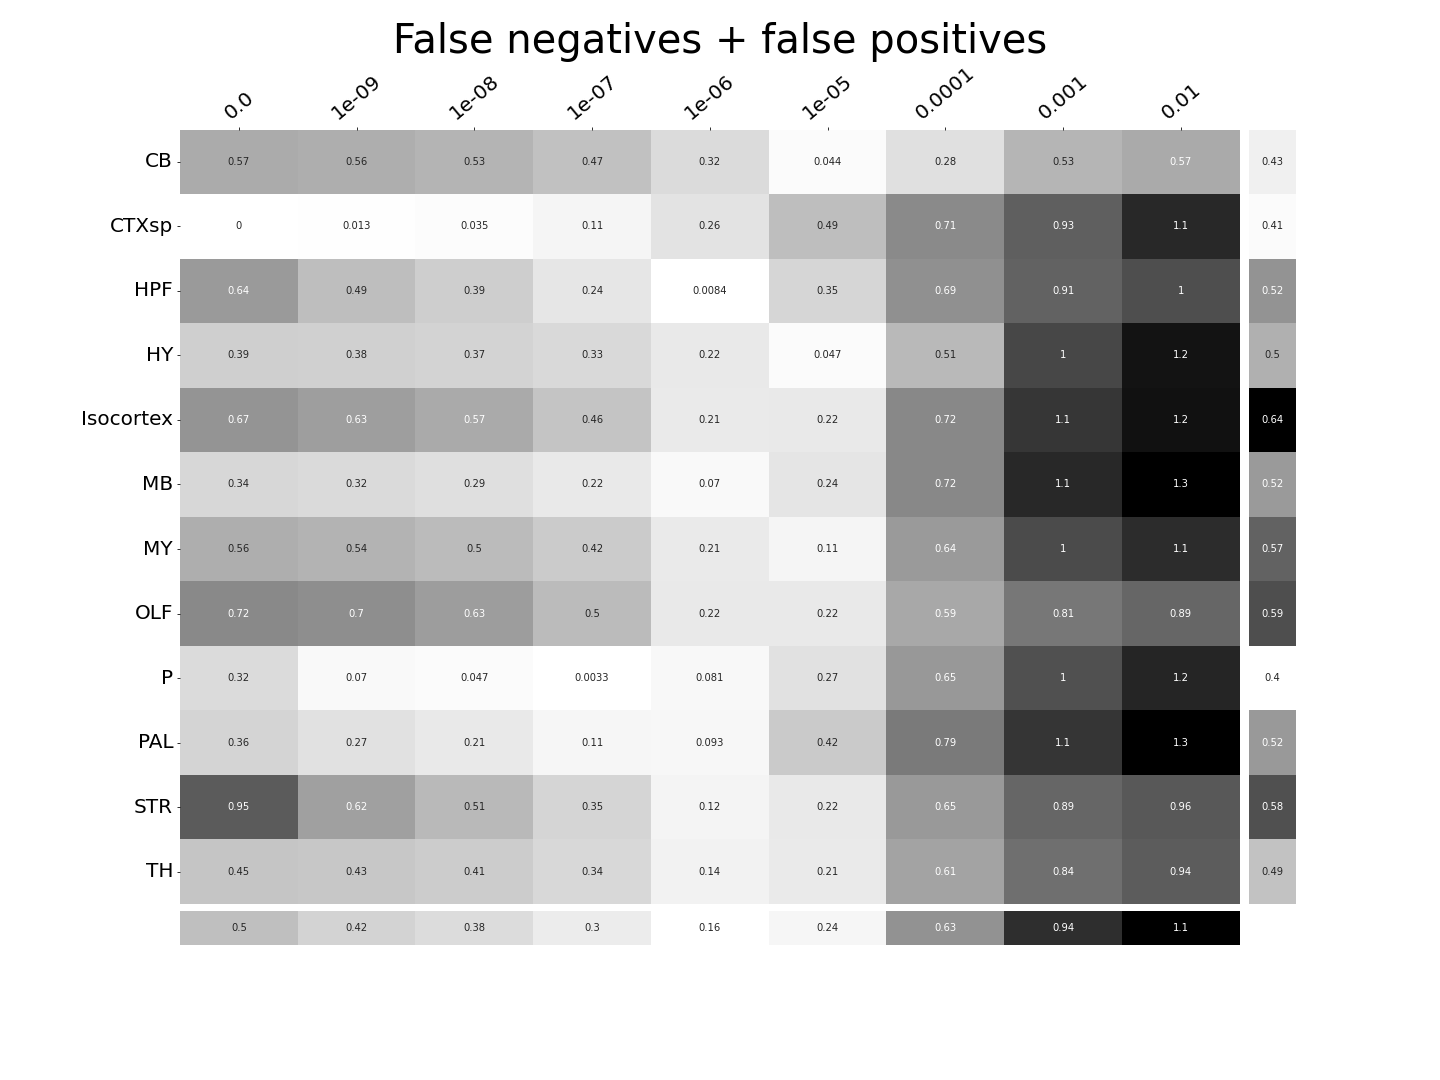
\includegraphics[width = 7in]{figs/Threshold.png}
    \label{fig:threshold}
    \caption{$\tau$ at different limits of detection in different major structures.  $10^{-6}$ is the optimal detection threshold.}
\end{figure}

\newpage

\subsection{Loss subsets}
\label{supp_sec:loss_subsets}

We report model accuracies for our $EL$ model by neuron class and structure.
These expand upon the results in Table \ref{tab:crossvalidation} and give more specific information about the quality of our estimates.   CTXsp is omitted due to the small nature of the evaluation set.

\begin{figure}[H]
    \centering
    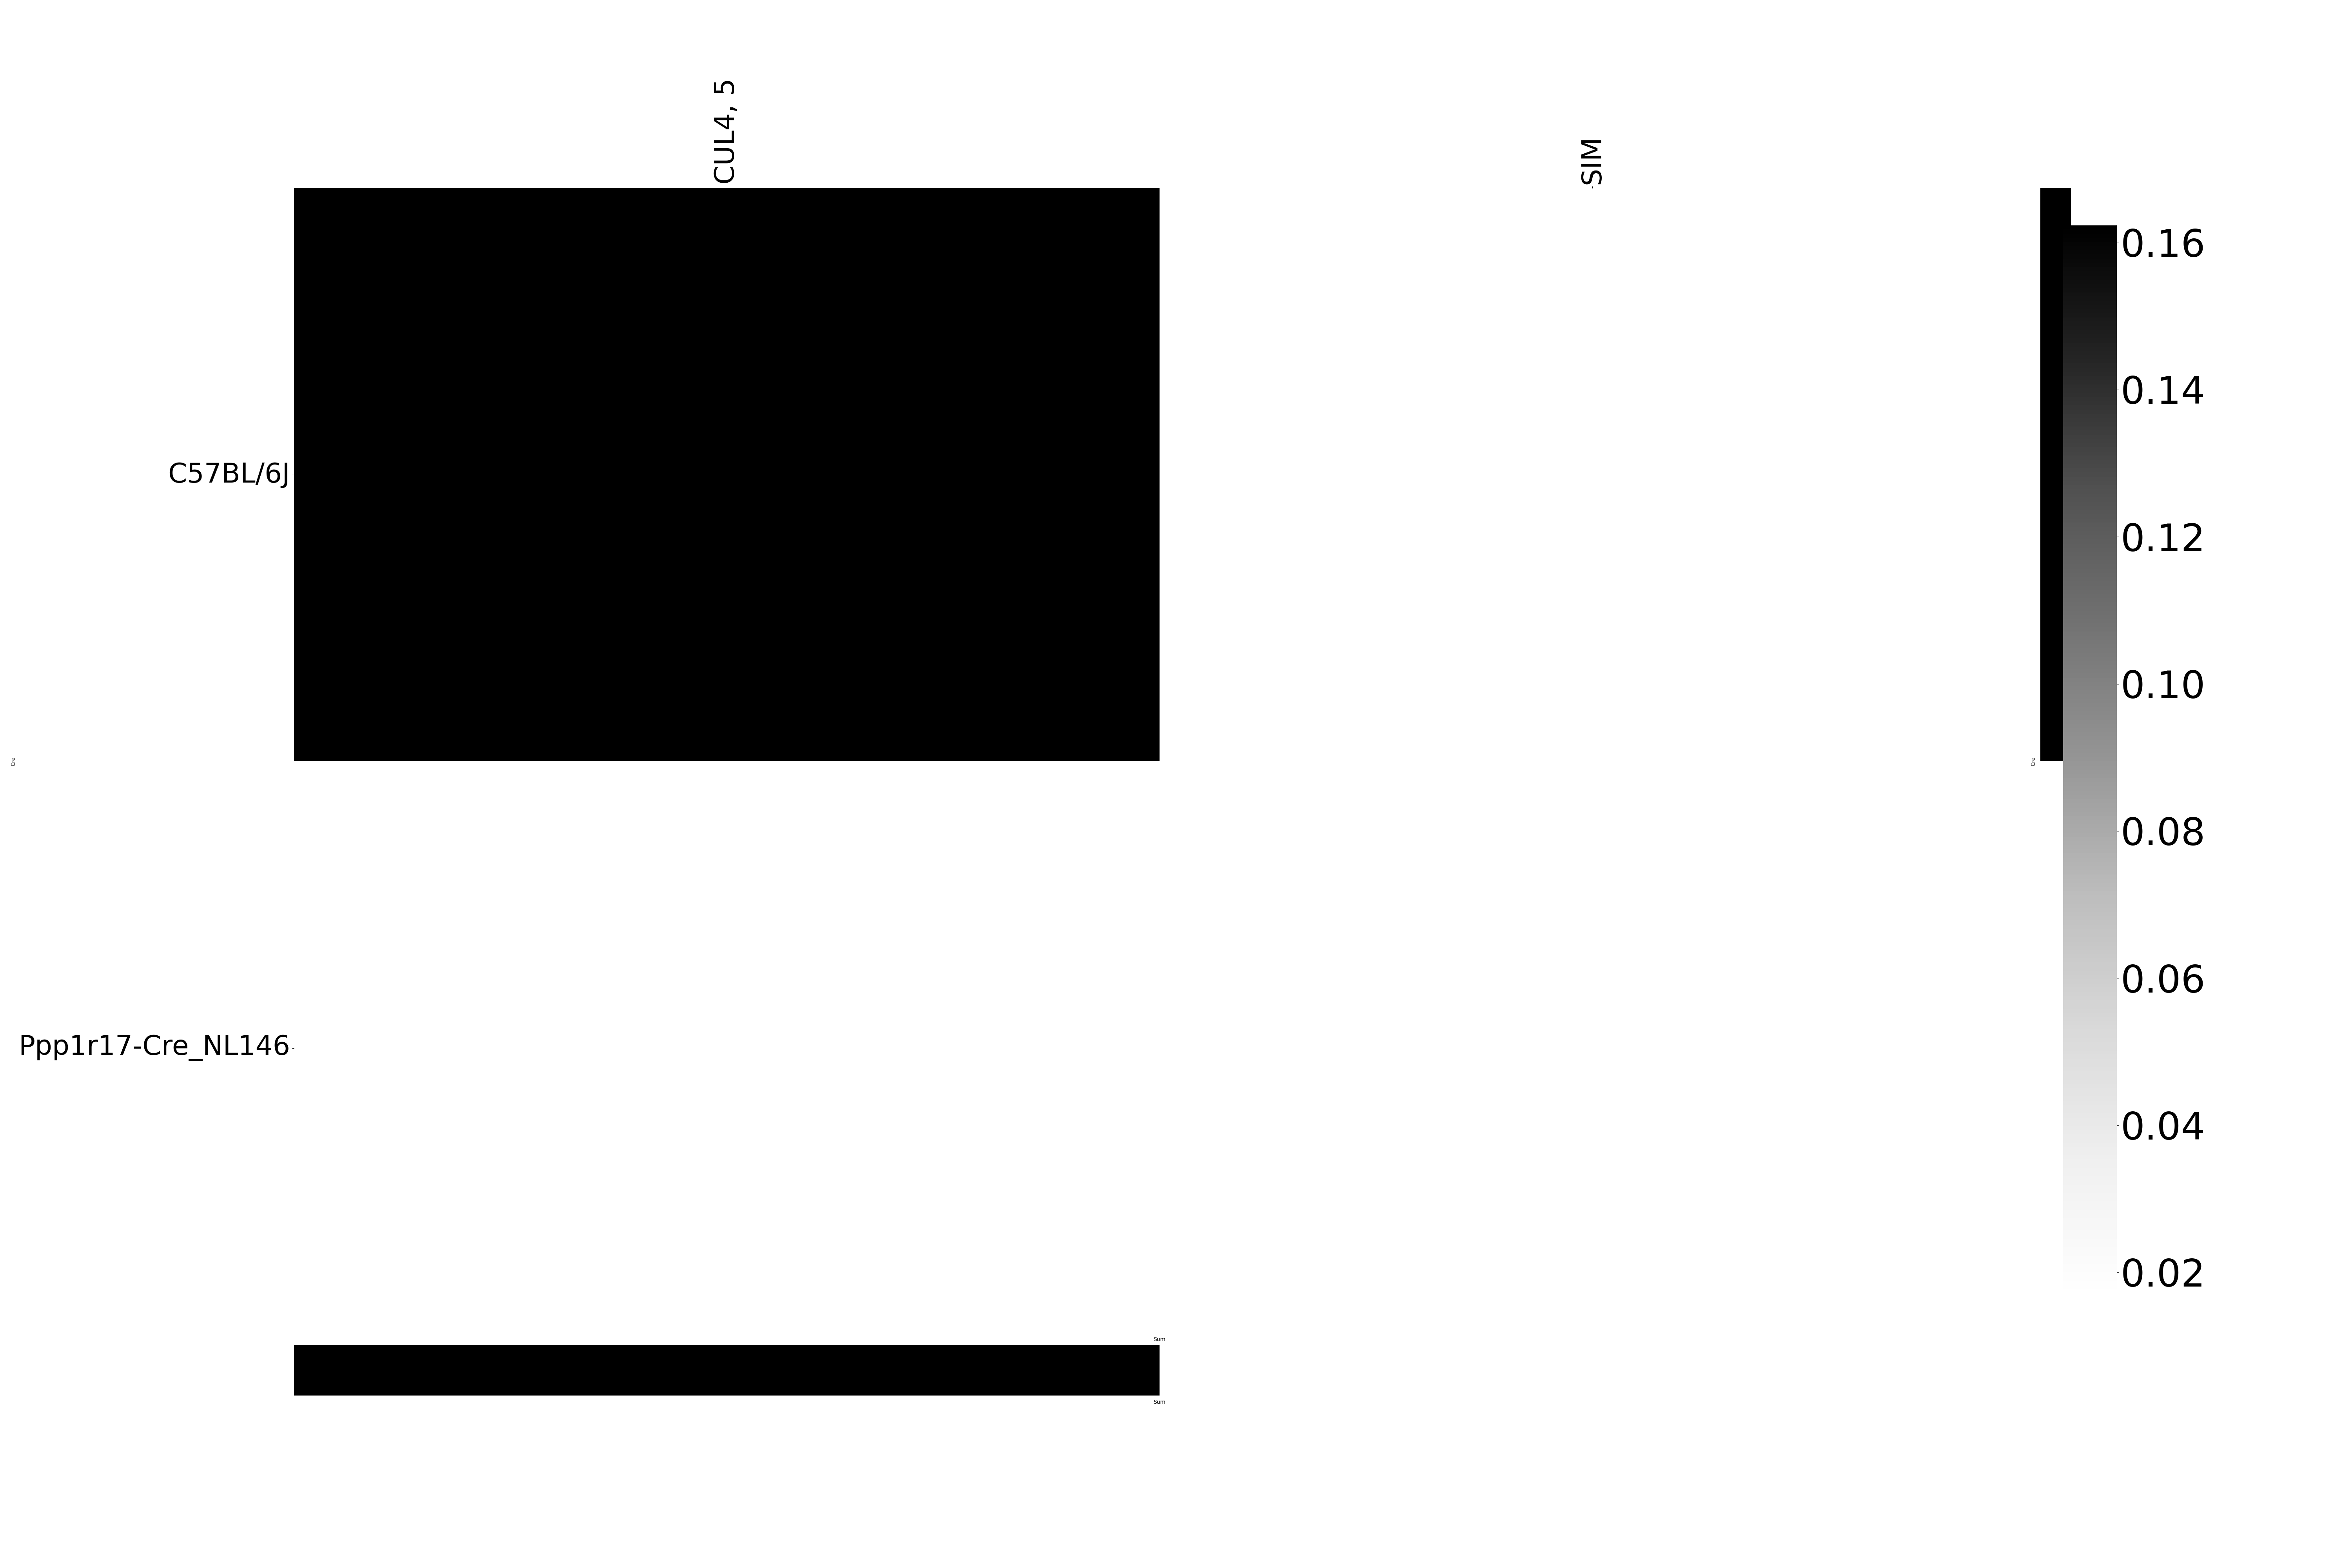
\includegraphics[width = 7in]{figs/lossdetails_512.png} 
    \label{fig:distances}
    \caption{Weighted loss for cre-leaf combinations in CB.  Missing values are omitted.   Row and column averages are also plotted.}
\end{figure}

%\begin{figure}[H]
 %   \centering
 %   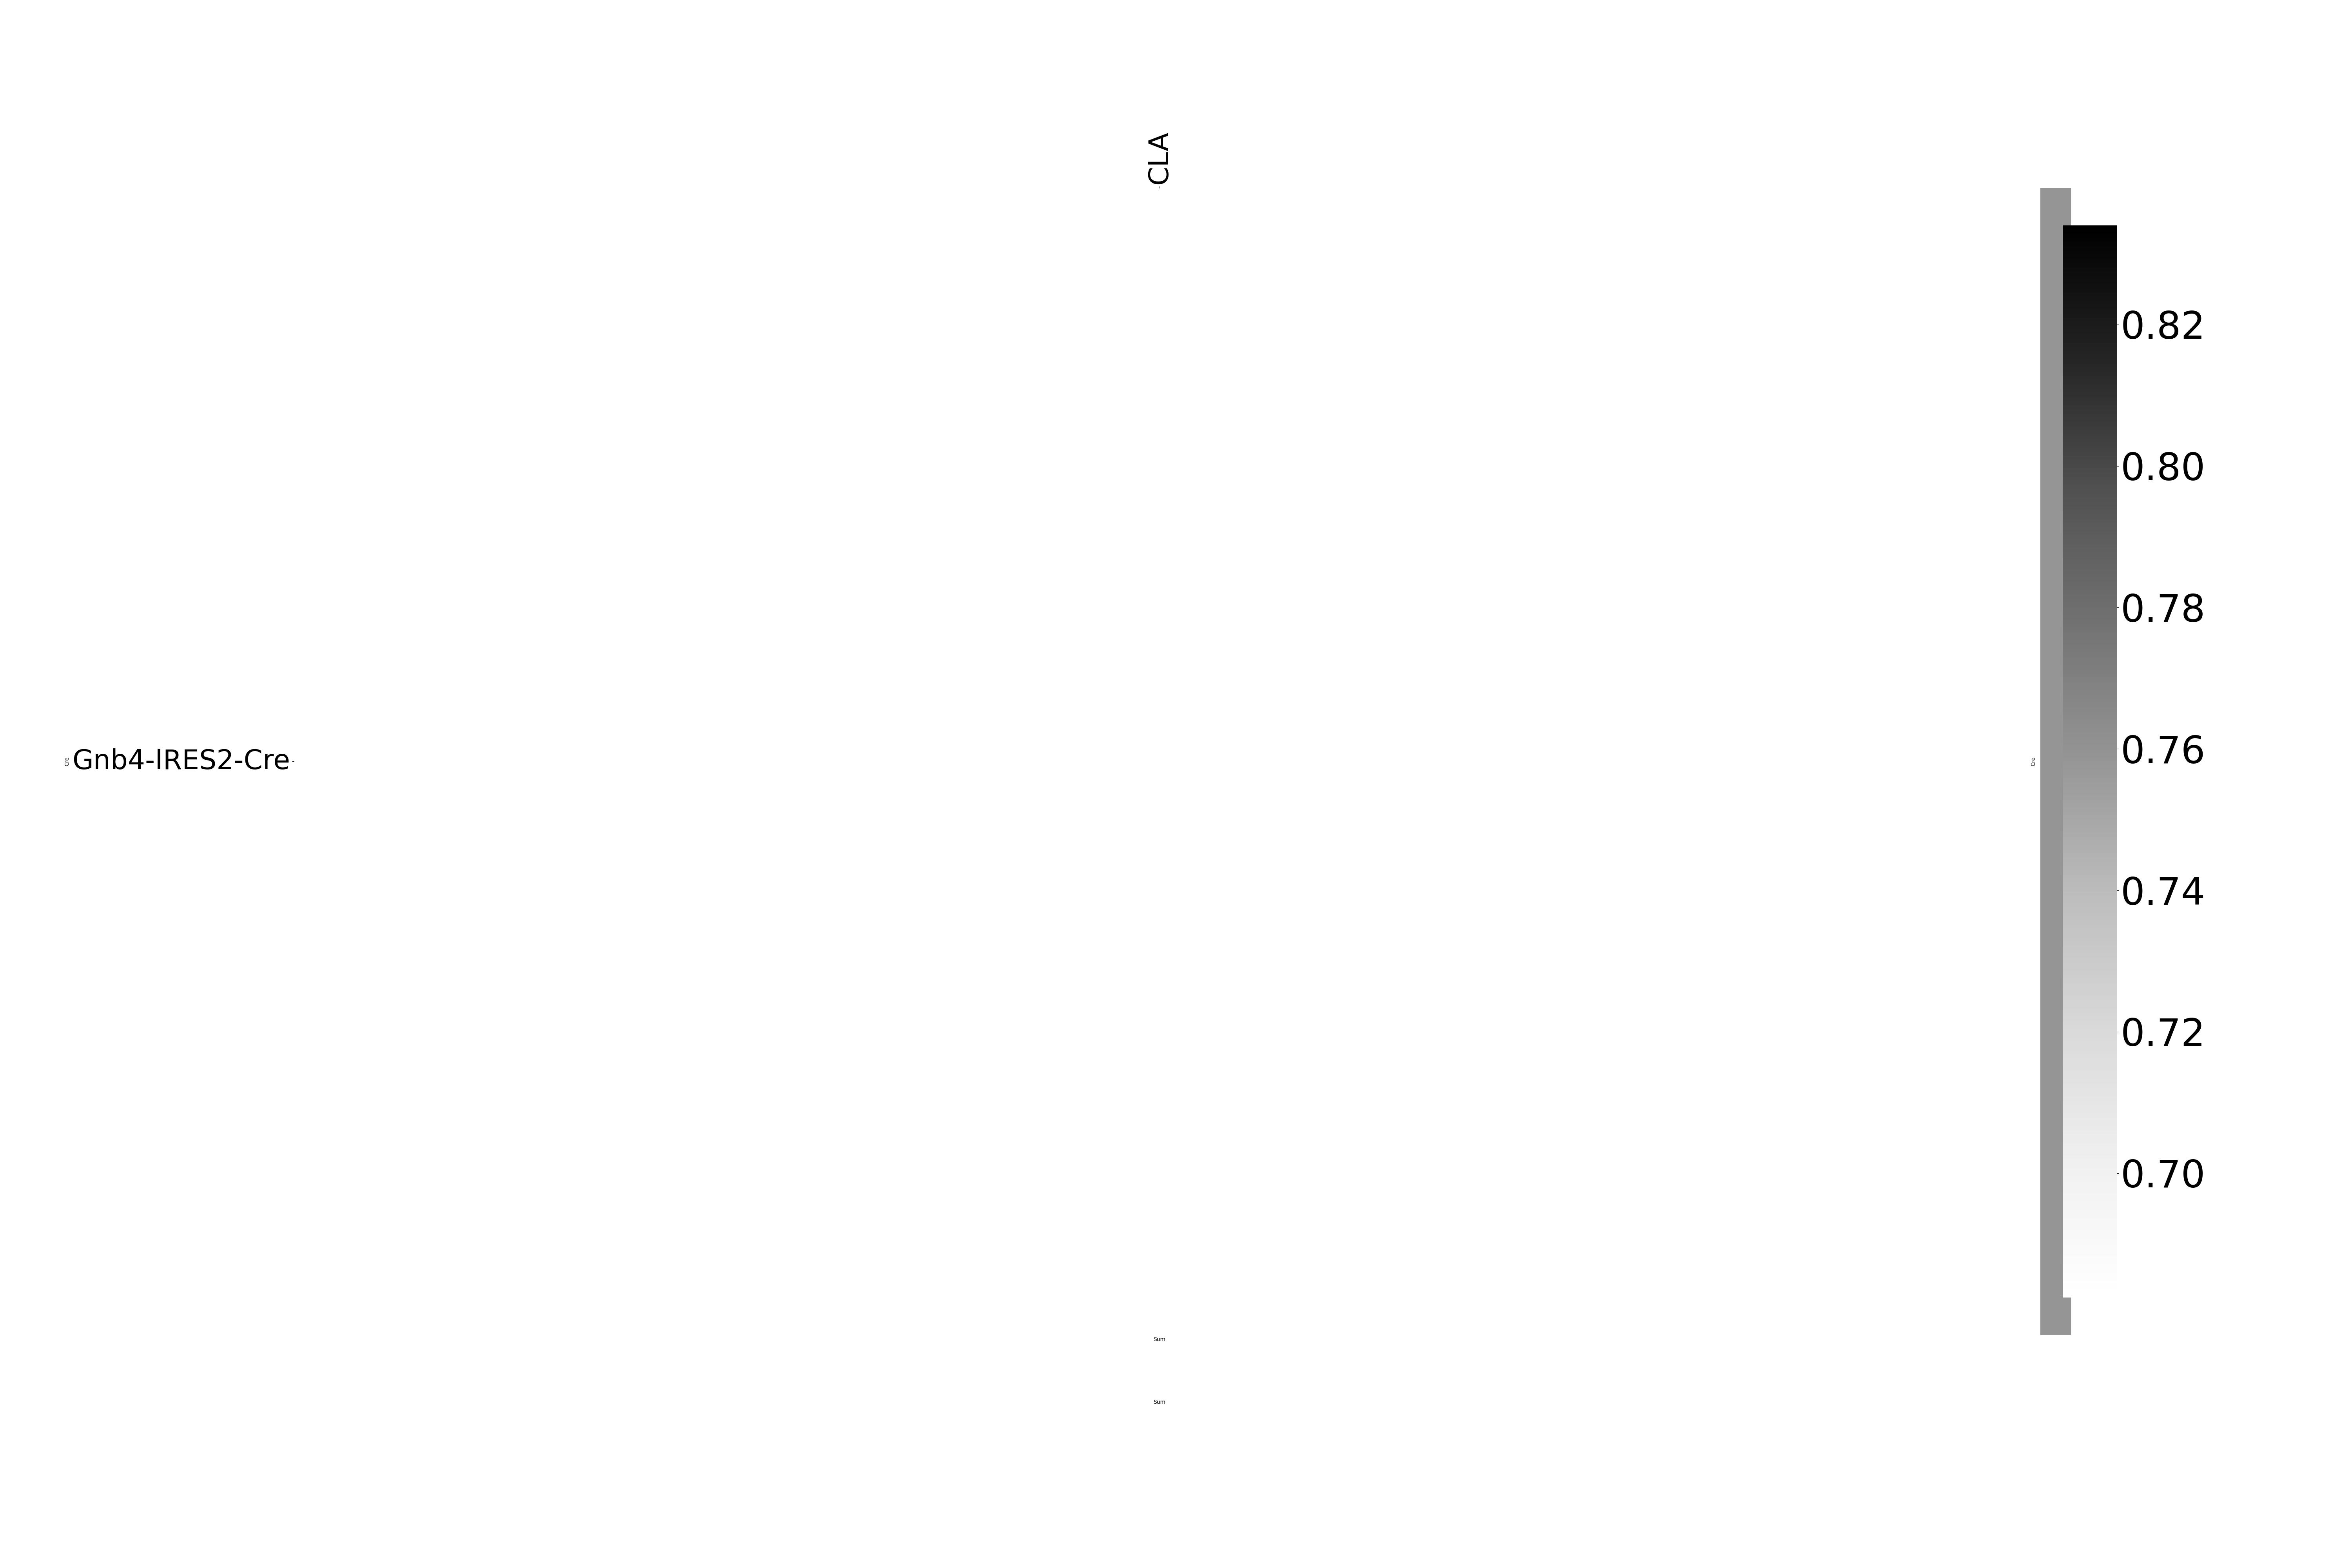
\includegraphics[width = 7in]{figs/lossdetails_703.png} 
 %   \label{fig:distances}
  %  \caption{Weighted loss for cre-leaf combinations in CTXsp.}
%\end{figure}

\begin{figure}[H]
    \centering
    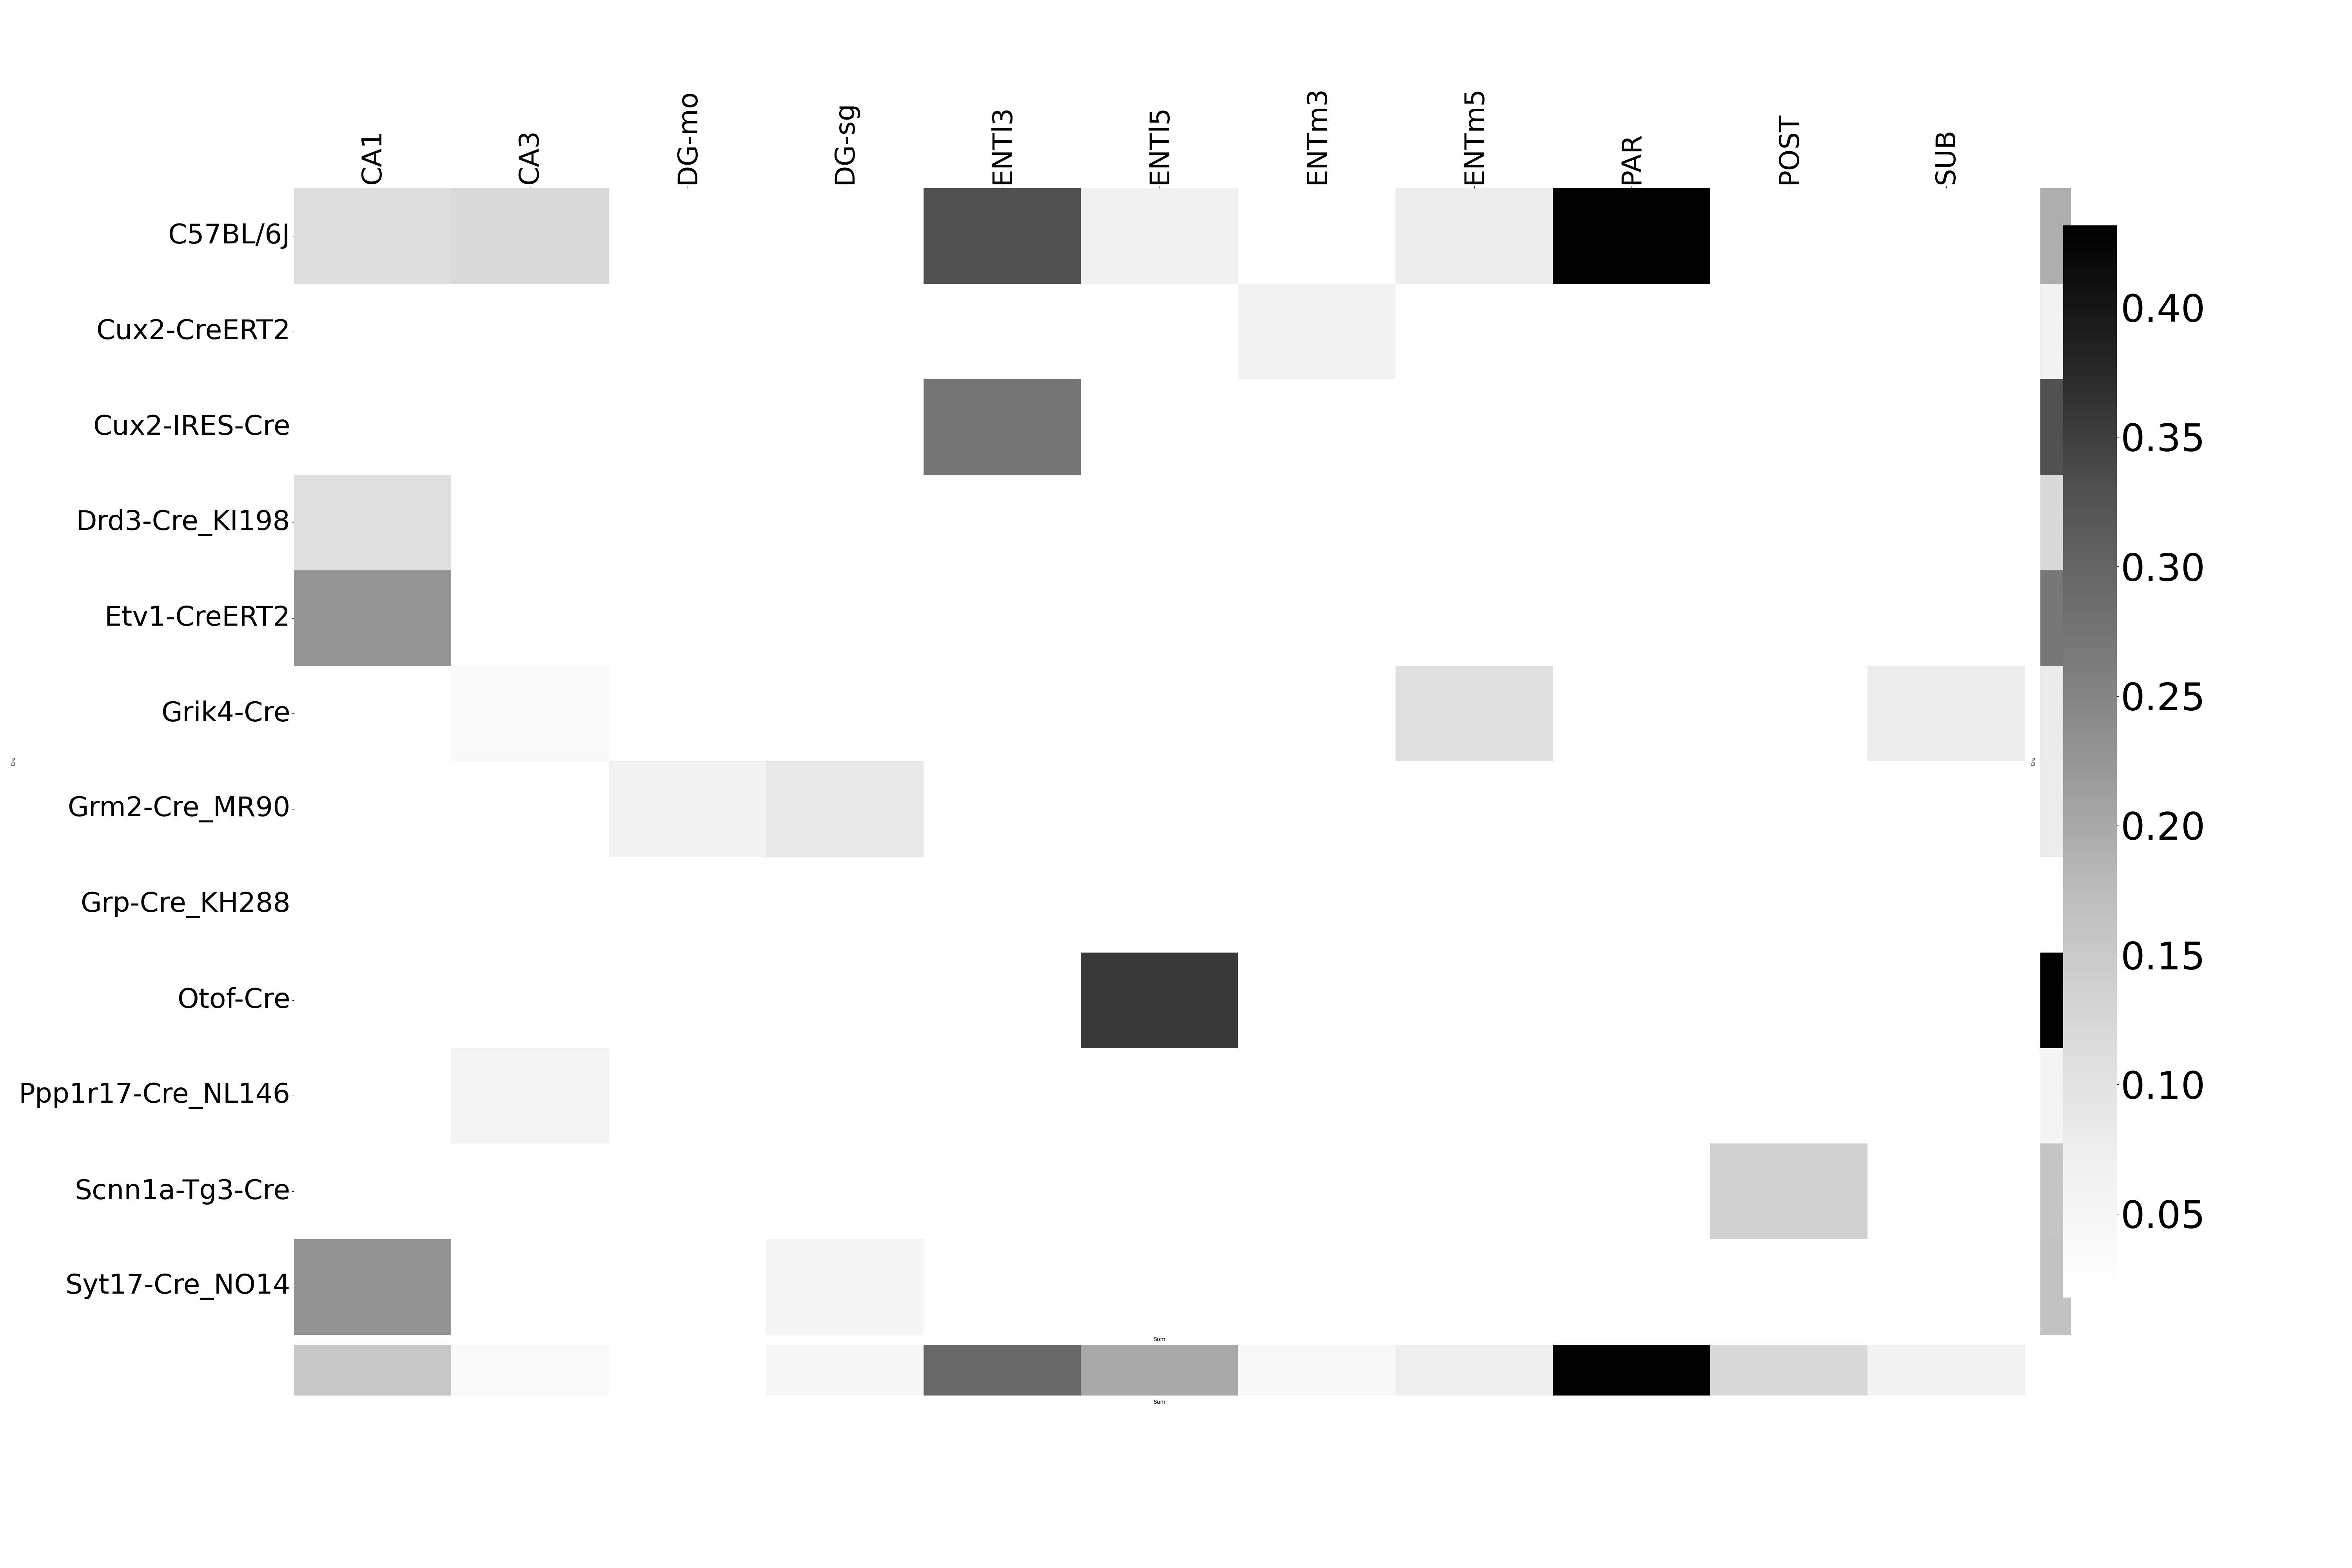
\includegraphics[width = 7in]{figs/lossdetails_1089.png} 
    \label{fig:distances}
    \caption{Weighted loss for cre-leaf combinations in HPF. Missing values are omitted.   Row and column averages are also plotted.}
\end{figure}

\begin{figure}[H]
    \centering
    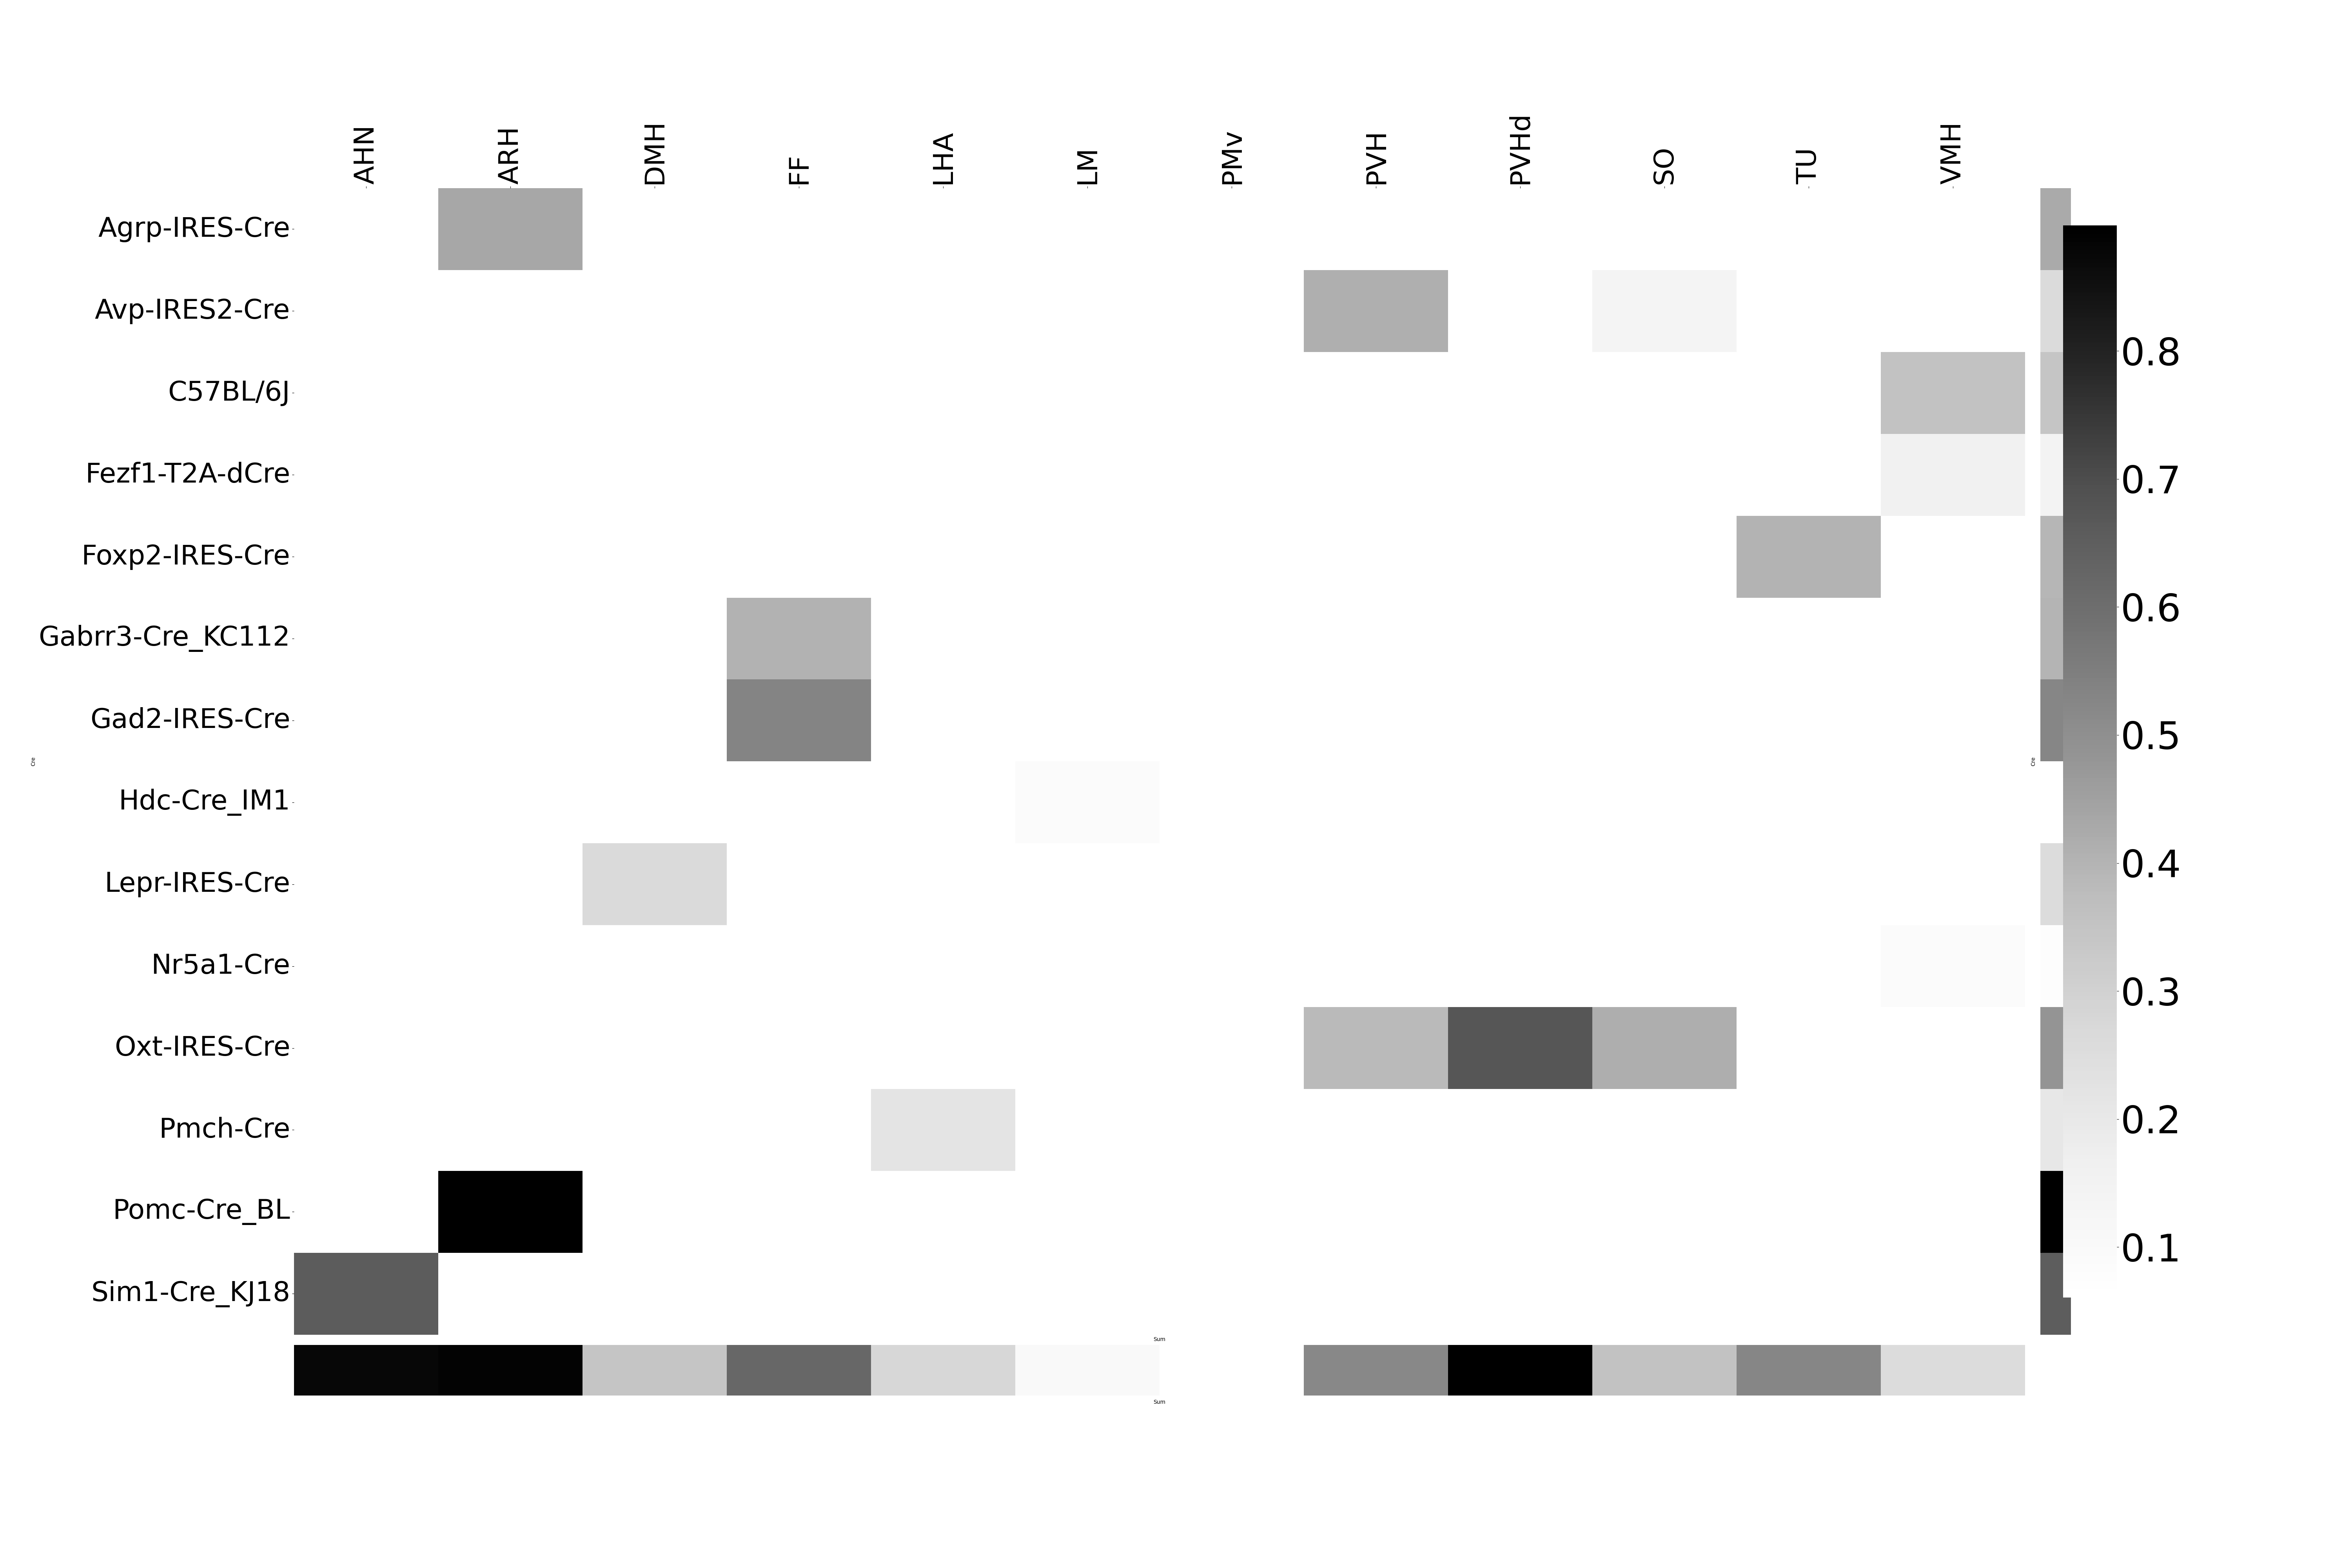
\includegraphics[width = 7in]{figs/lossdetails_1097.png} 
    \label{fig:distances}
    \caption{Weighted loss for cre-leaf combinations in HY. Missing values are omitted.   Row and column averages are also plotted.}
\end{figure}

\begin{figure}[H]
    \centering
    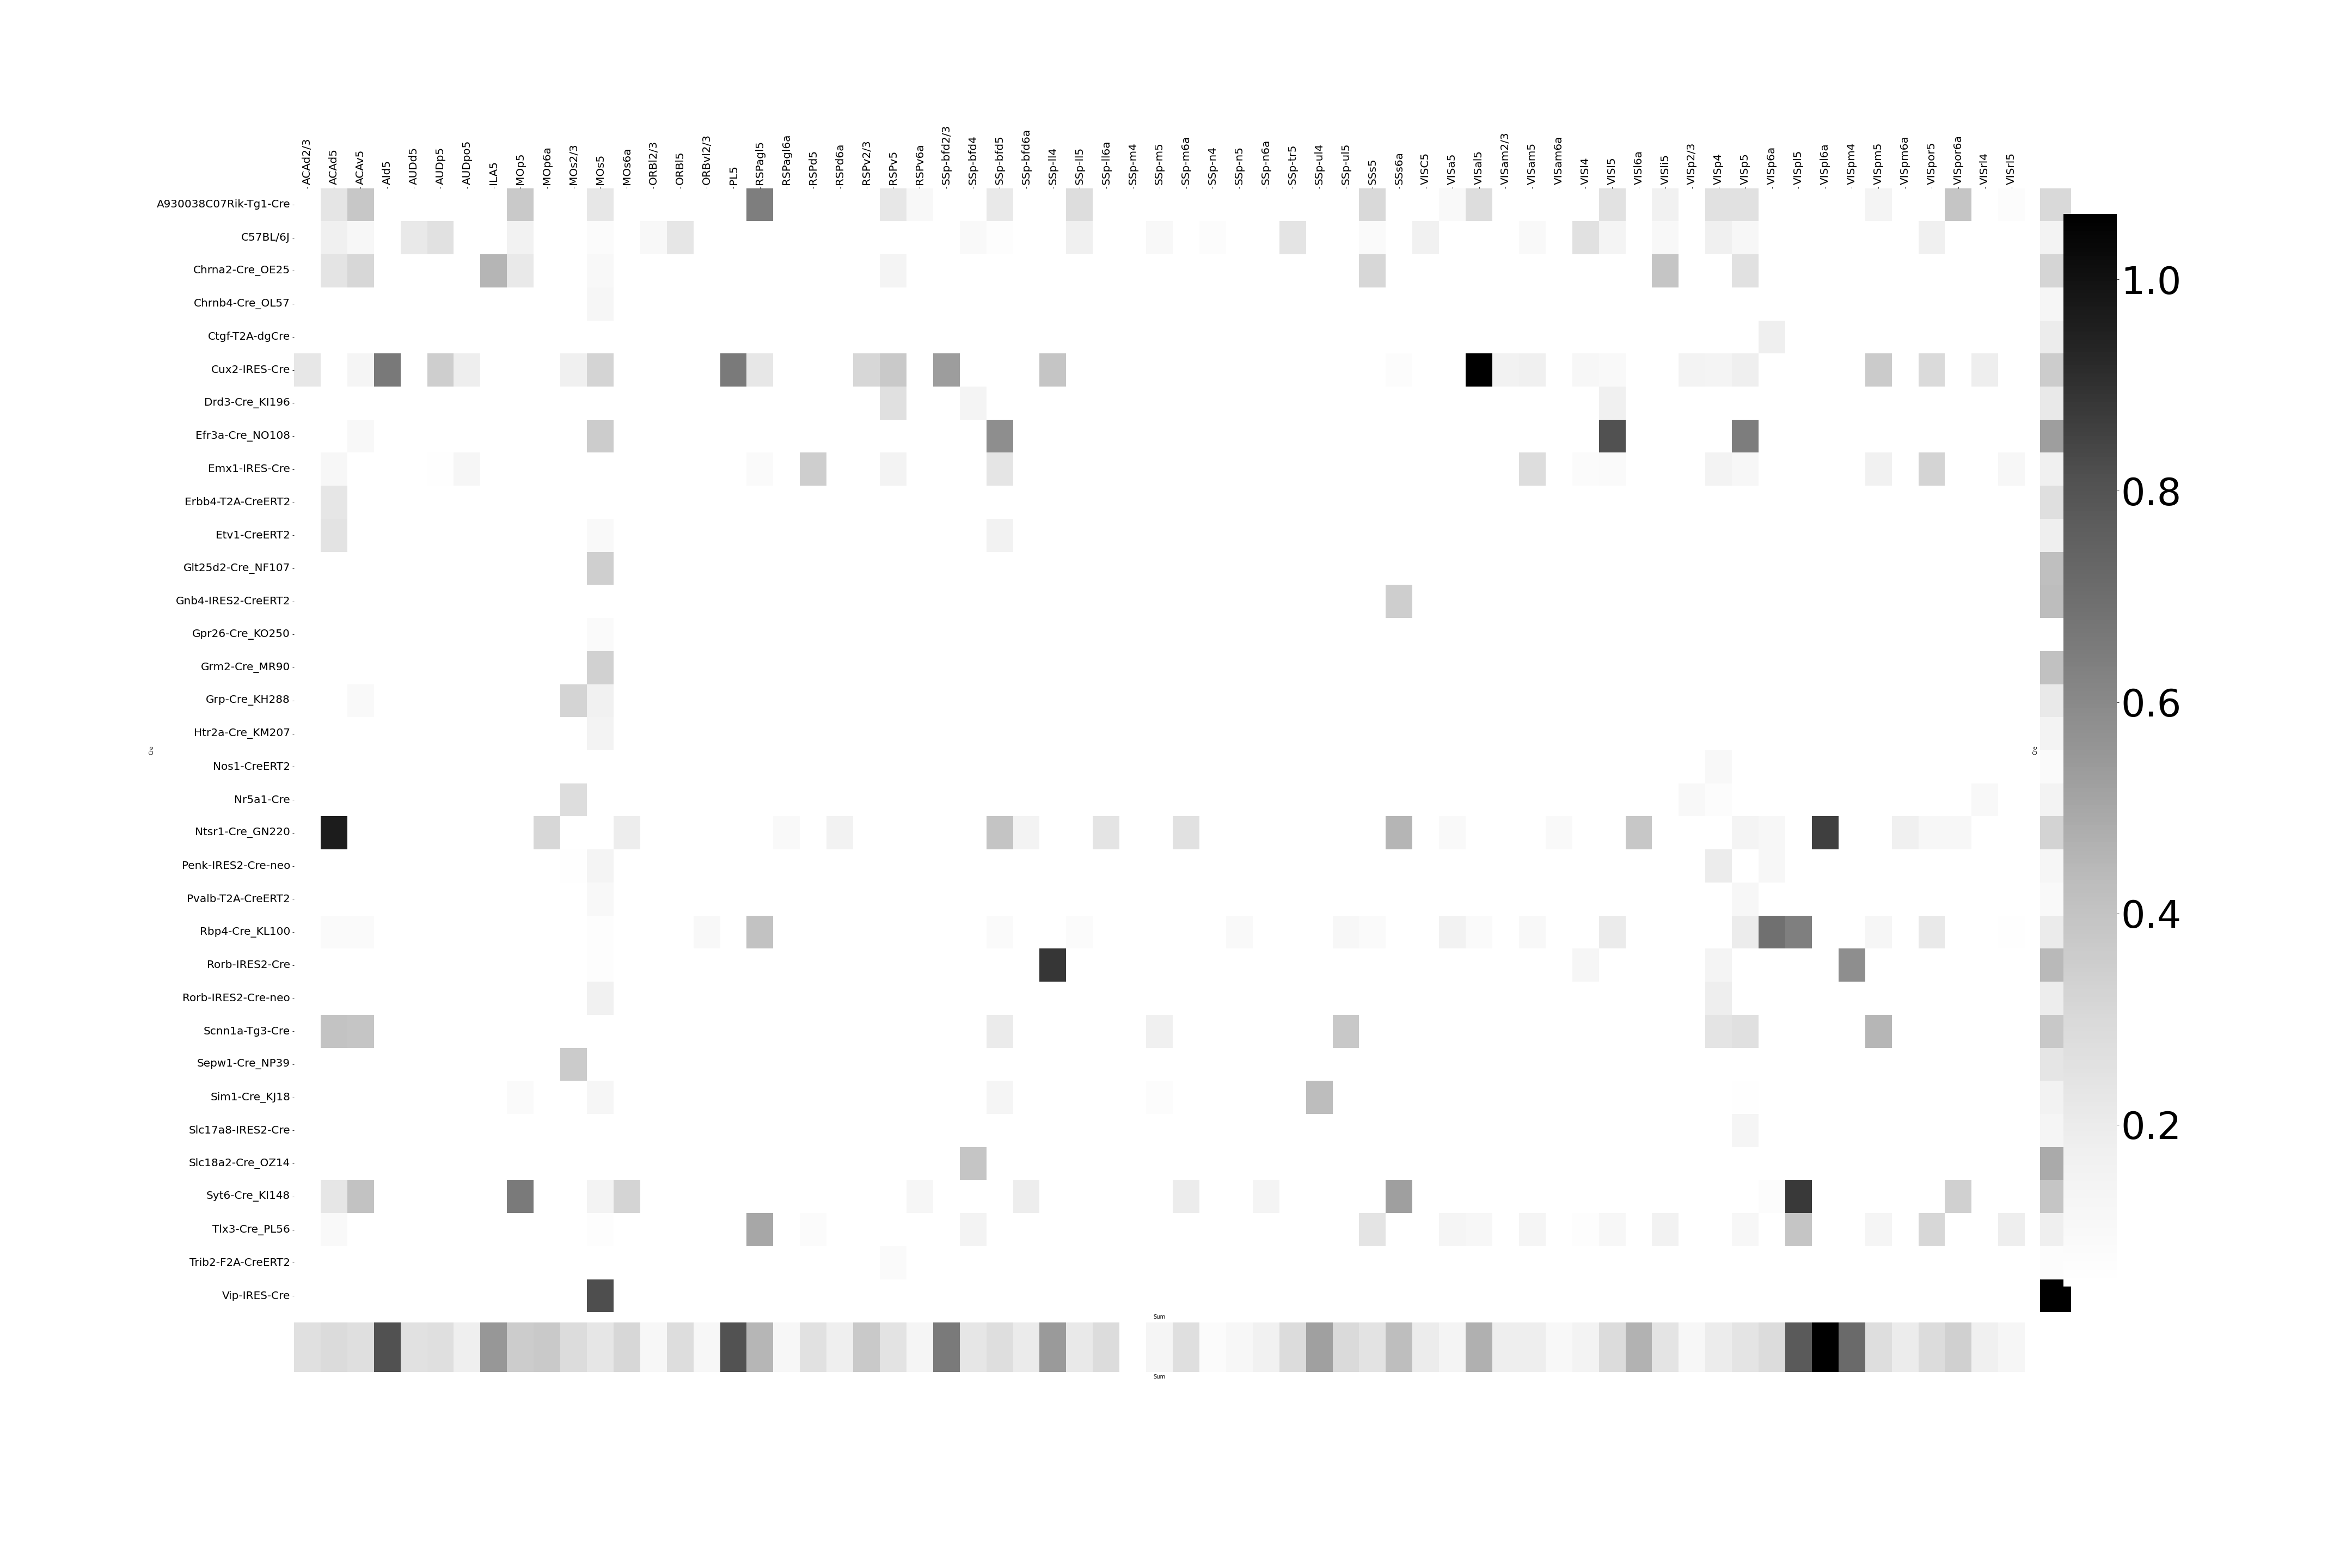
\includegraphics[width = 7in]{figs/lossdetails_315.png} 
    \label{fig:distances}
    \caption{Weighted loss for cre-leaf combinations in Isocortex. Missing values are omitted.  Row and column averages are also plotted.}
\end{figure}

\begin{figure}[H]
    \centering
    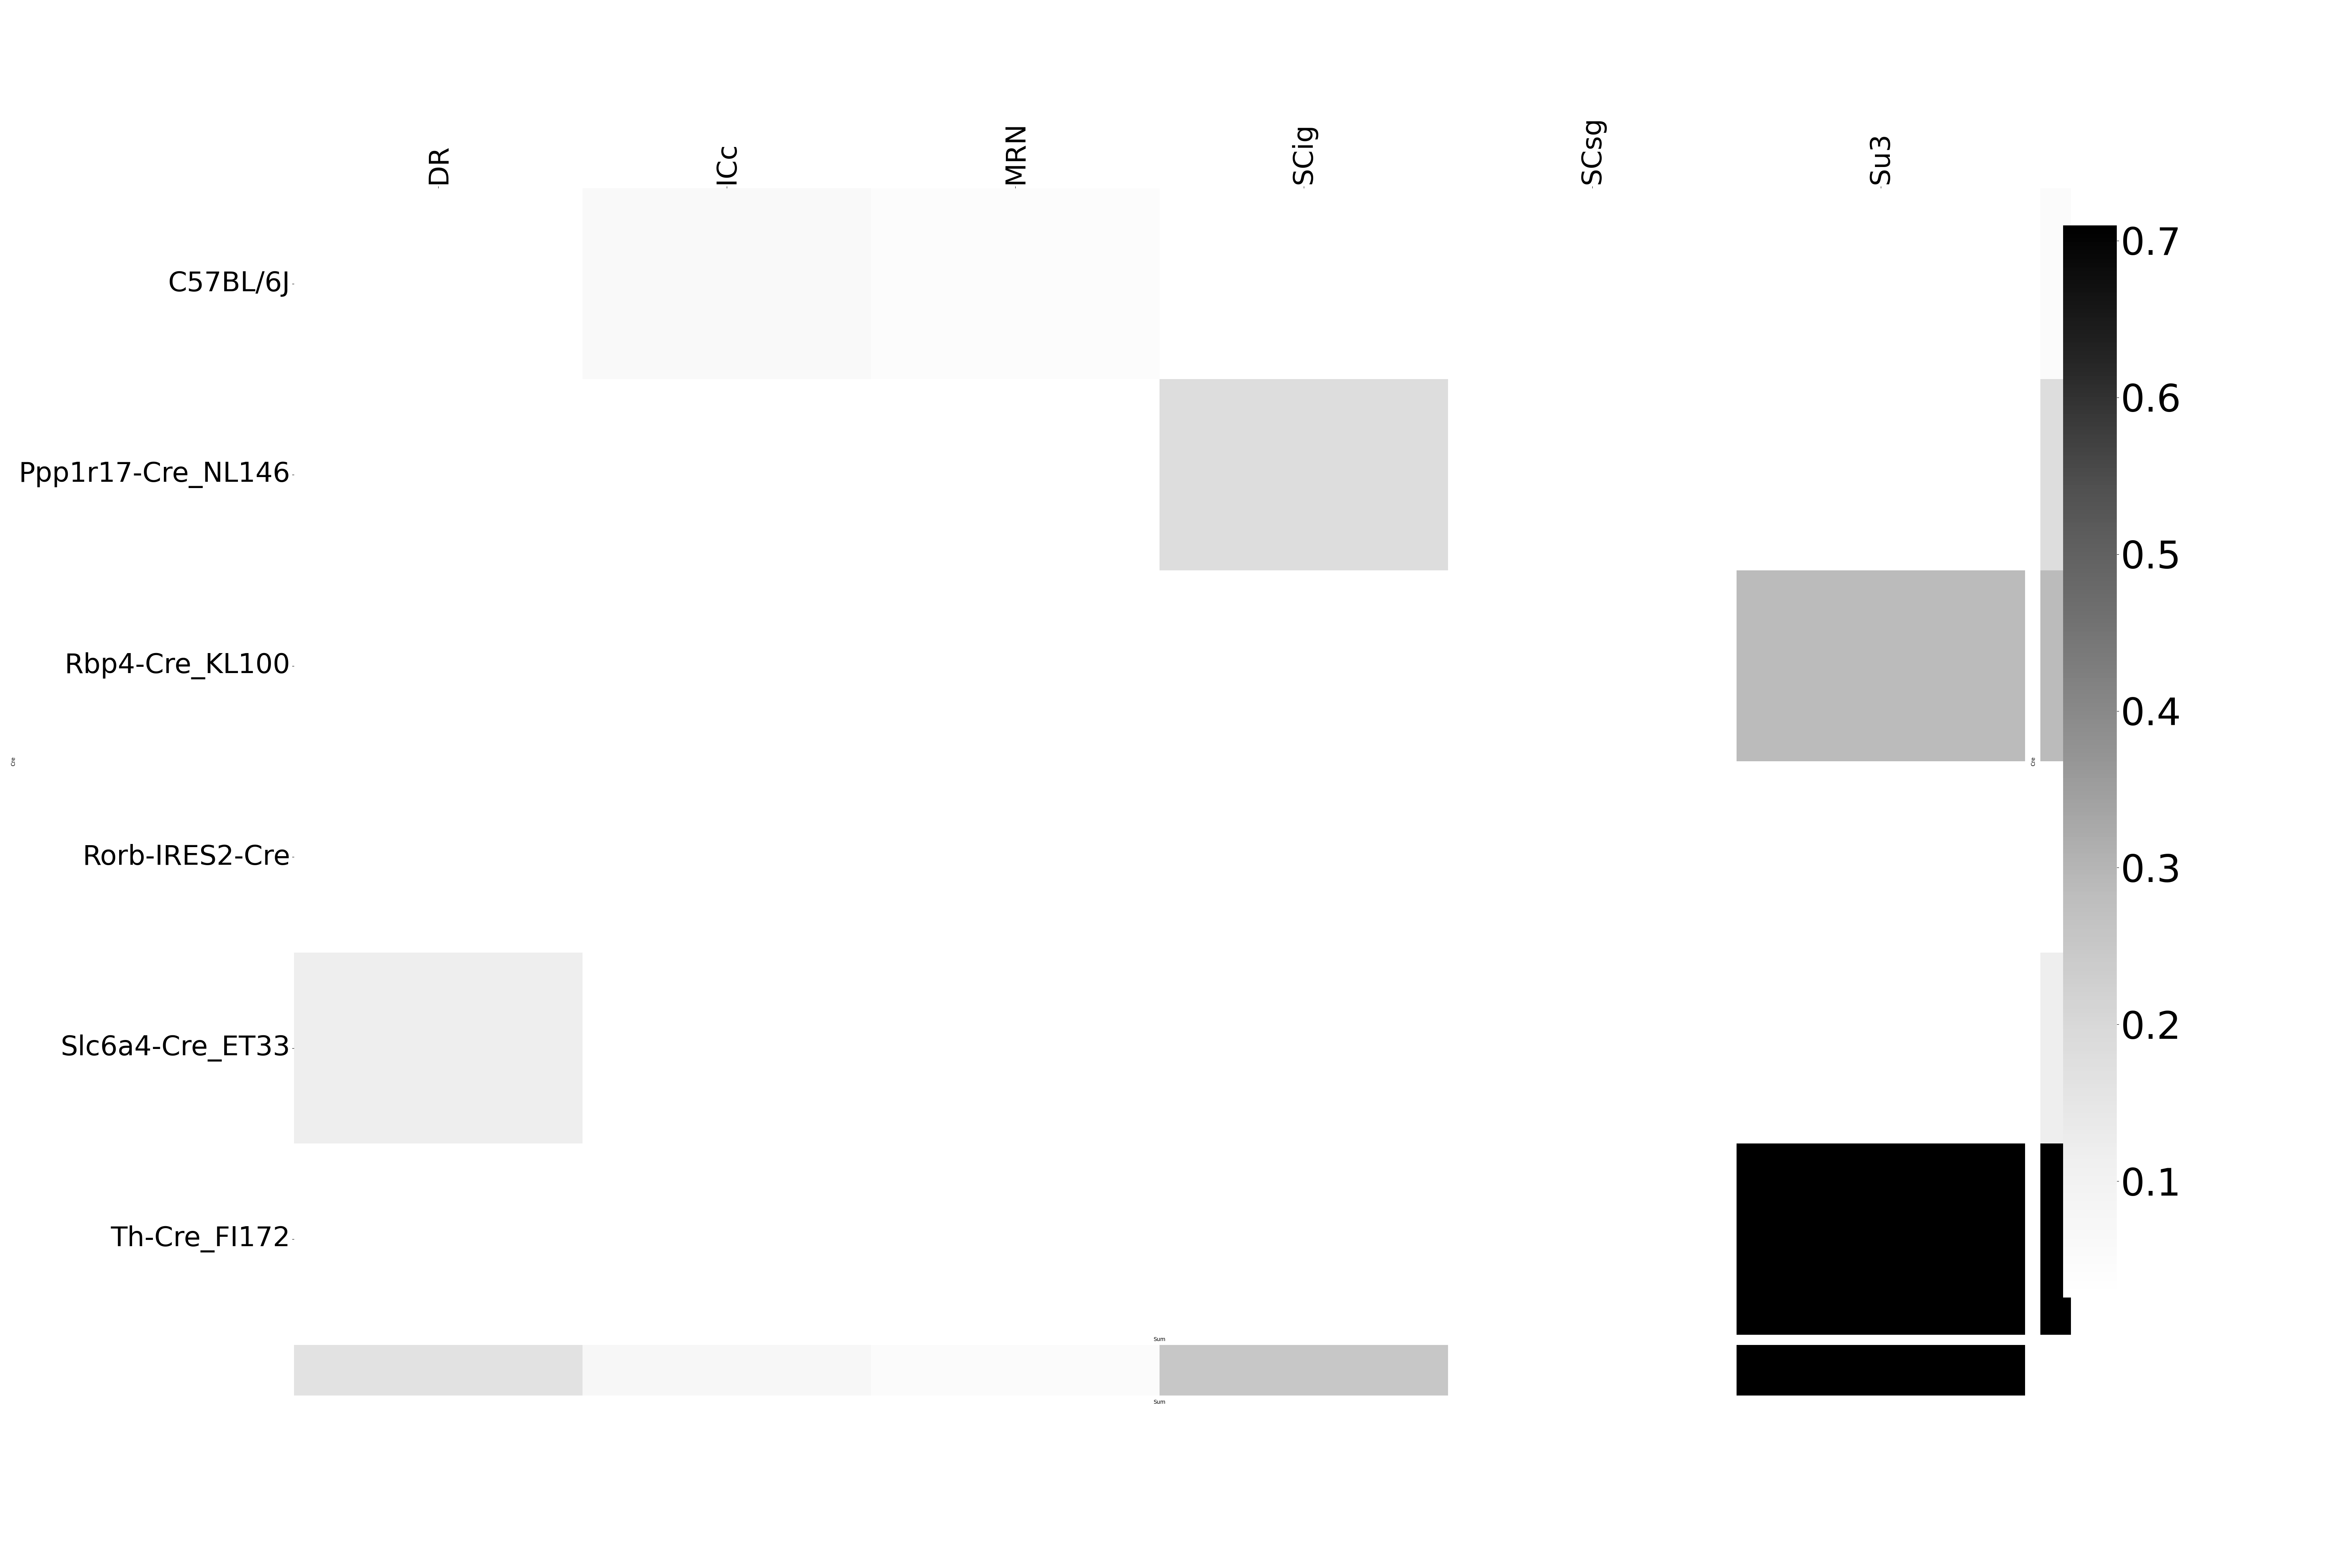
\includegraphics[width = 7in]{figs/lossdetails_313.png} 
    \label{fig:distances}
    \caption{Weighted loss for cre-leaf combinations in MB. Missing values are omitted.   Row and column averages are also plotted.}
\end{figure}

\begin{figure}[H]
    \centering
    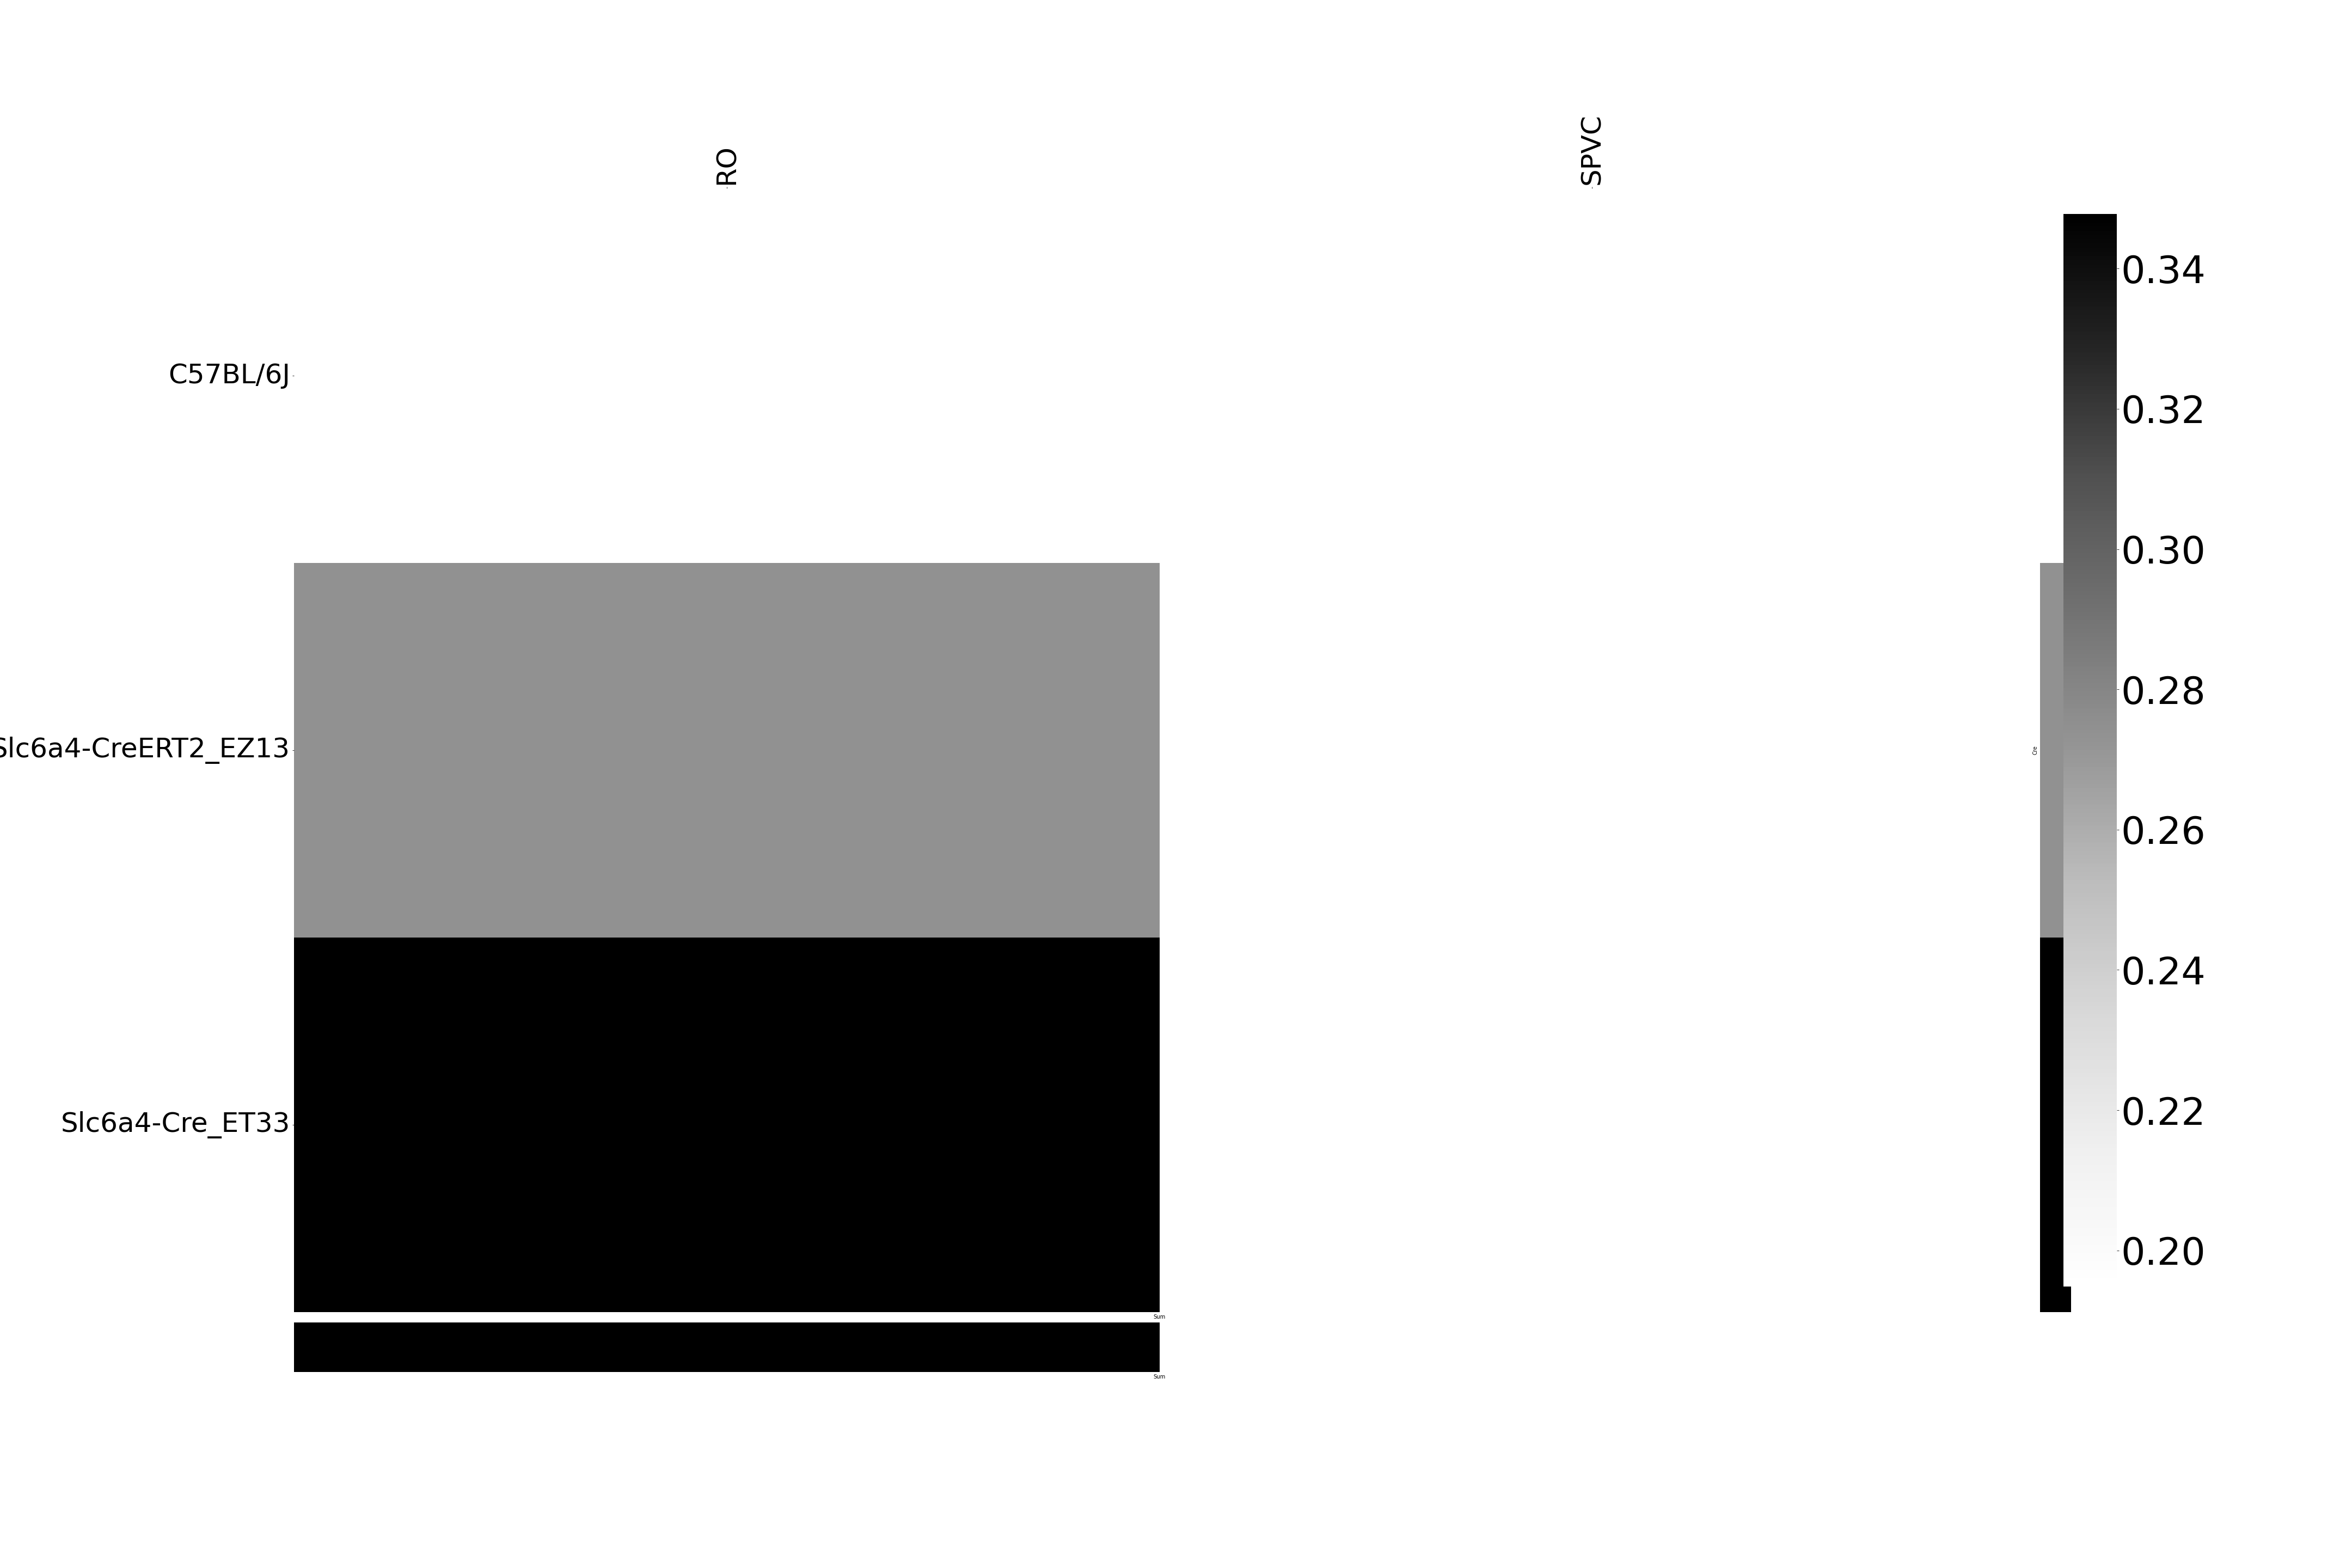
\includegraphics[width = 7in]{figs/lossdetails_354.png} 
    \label{fig:distances}
    \caption{Weighted loss for cre-leaf combinations in MY. Missing values are omitted.   Row and column averages are also plotted.}
\end{figure}

\begin{figure}[H]
    \centering
    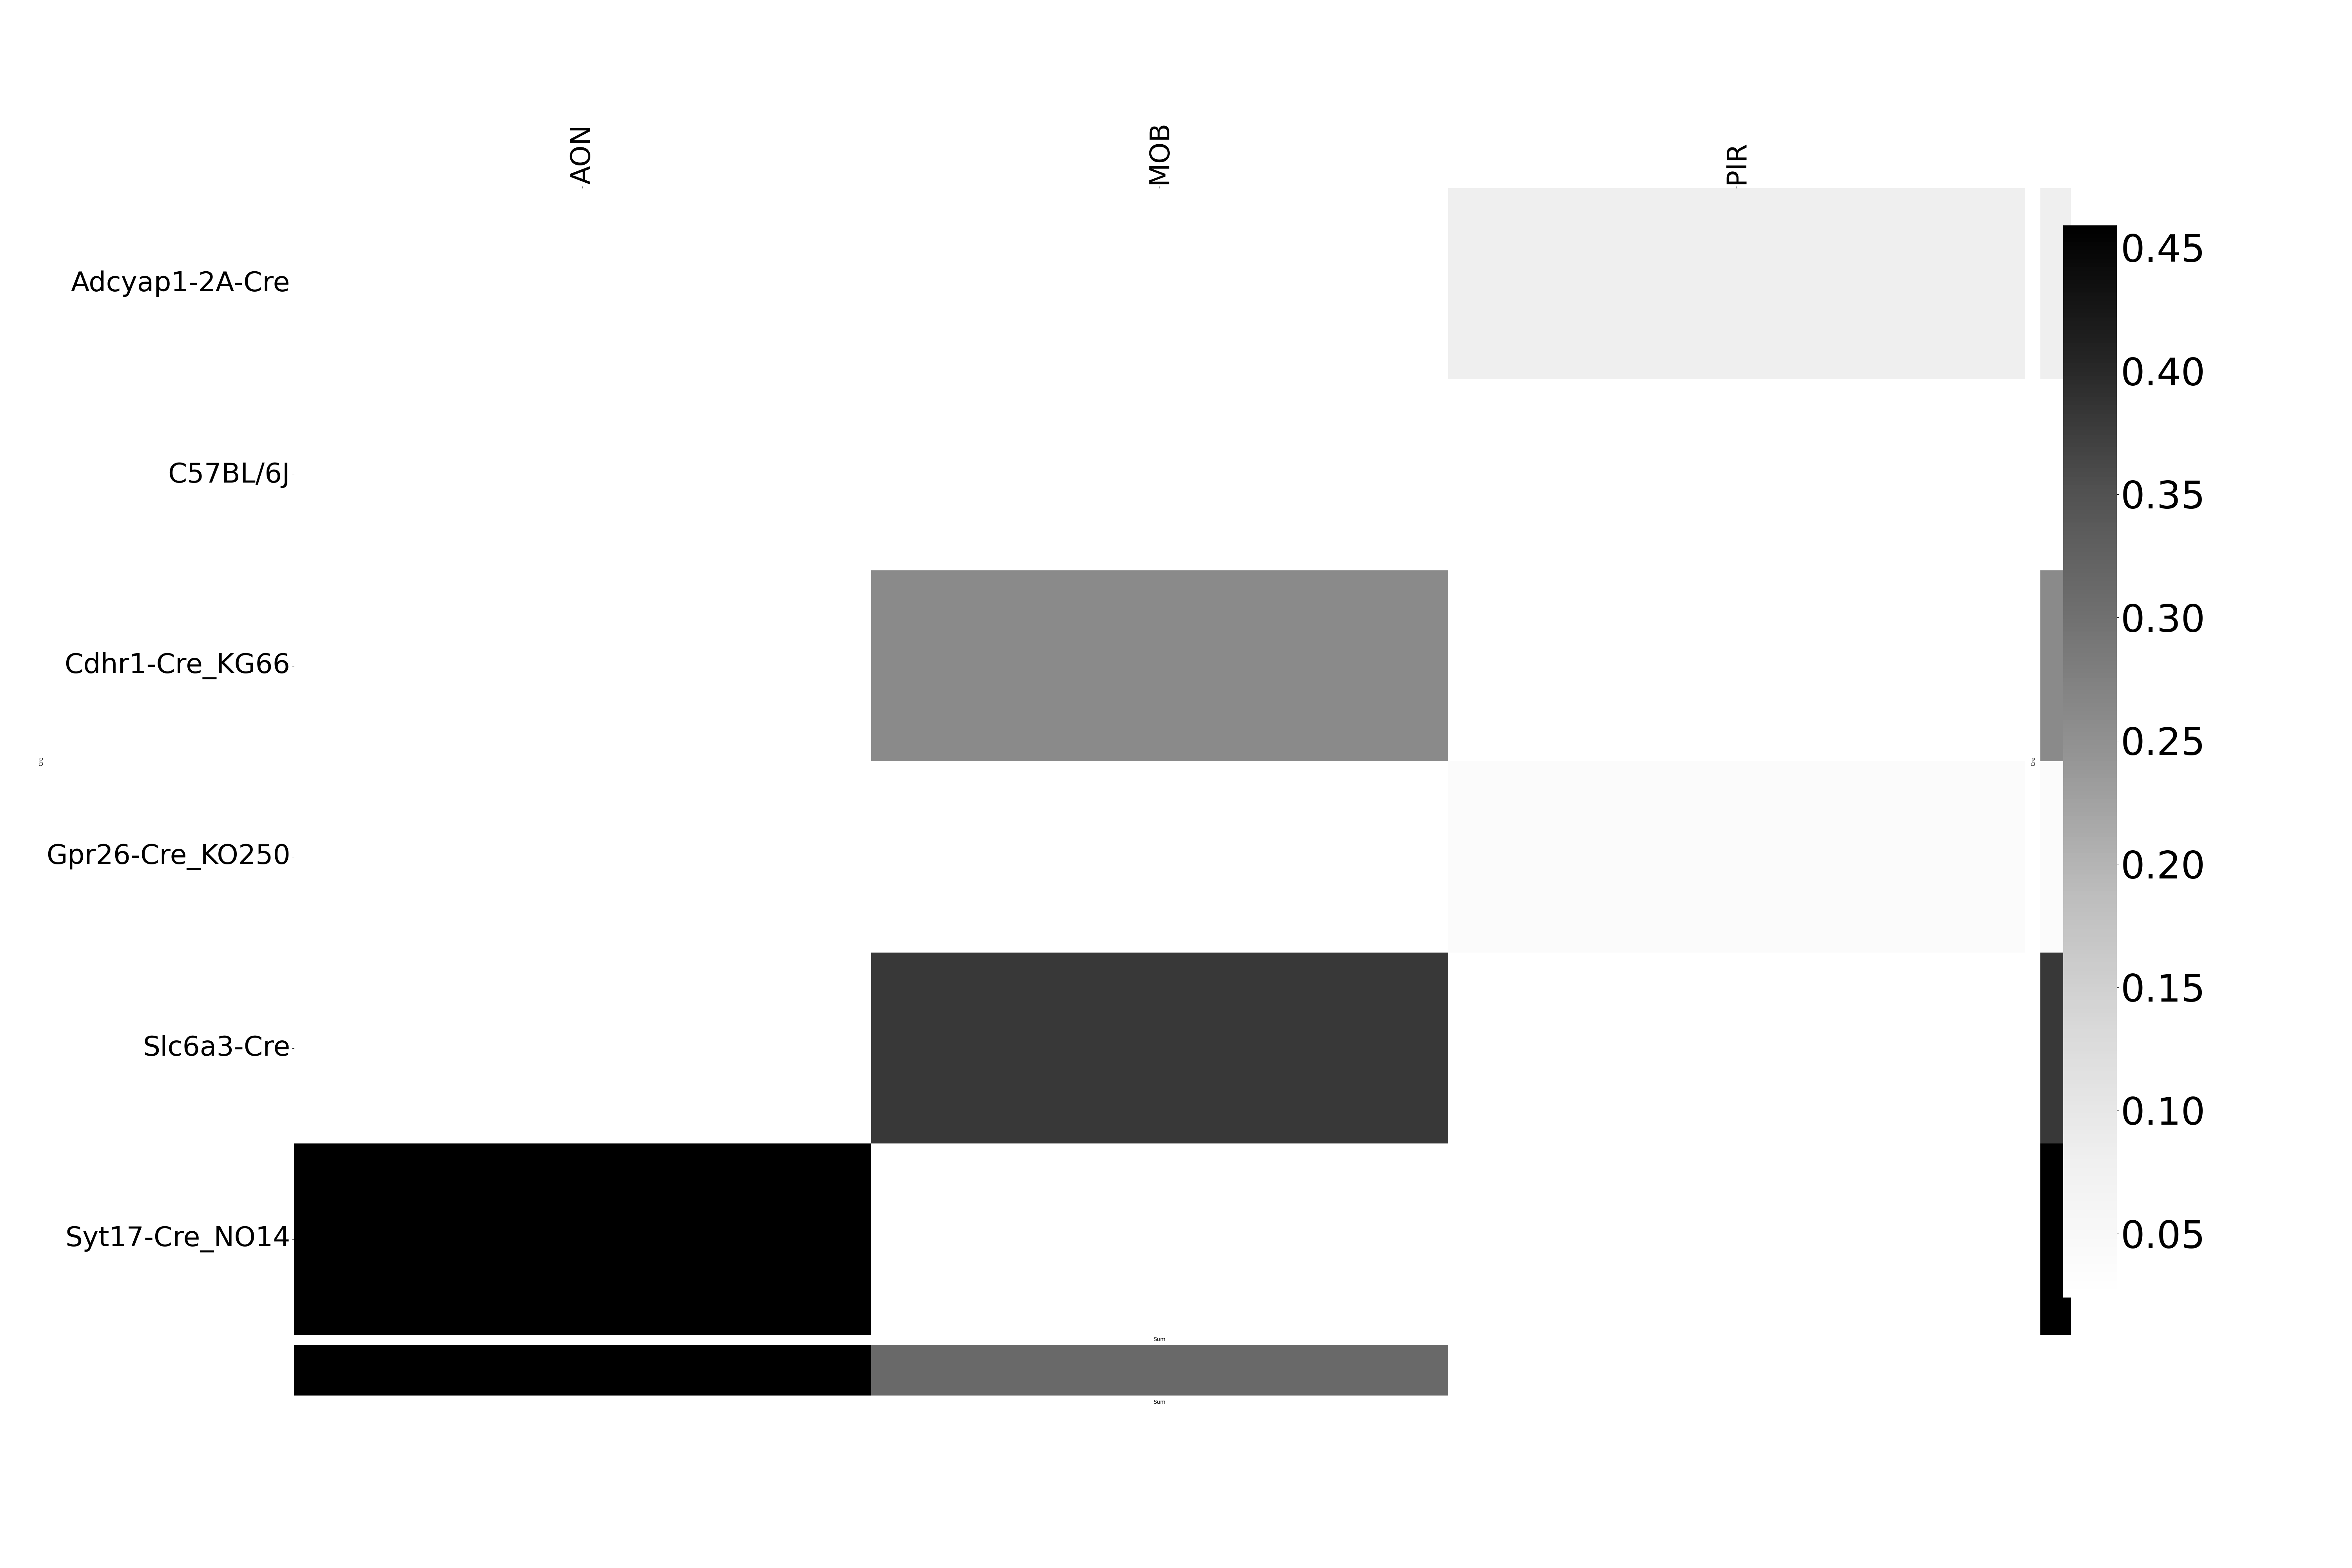
\includegraphics[width = 7in]{figs/lossdetails_698.png} 
    \label{fig:distances}
    \caption{Weighted loss for cre-leaf combinations in OLF.  Missing values are omitted.   Row and column averages are also plotted.}
\end{figure}

\begin{figure}[H]
    \centering
    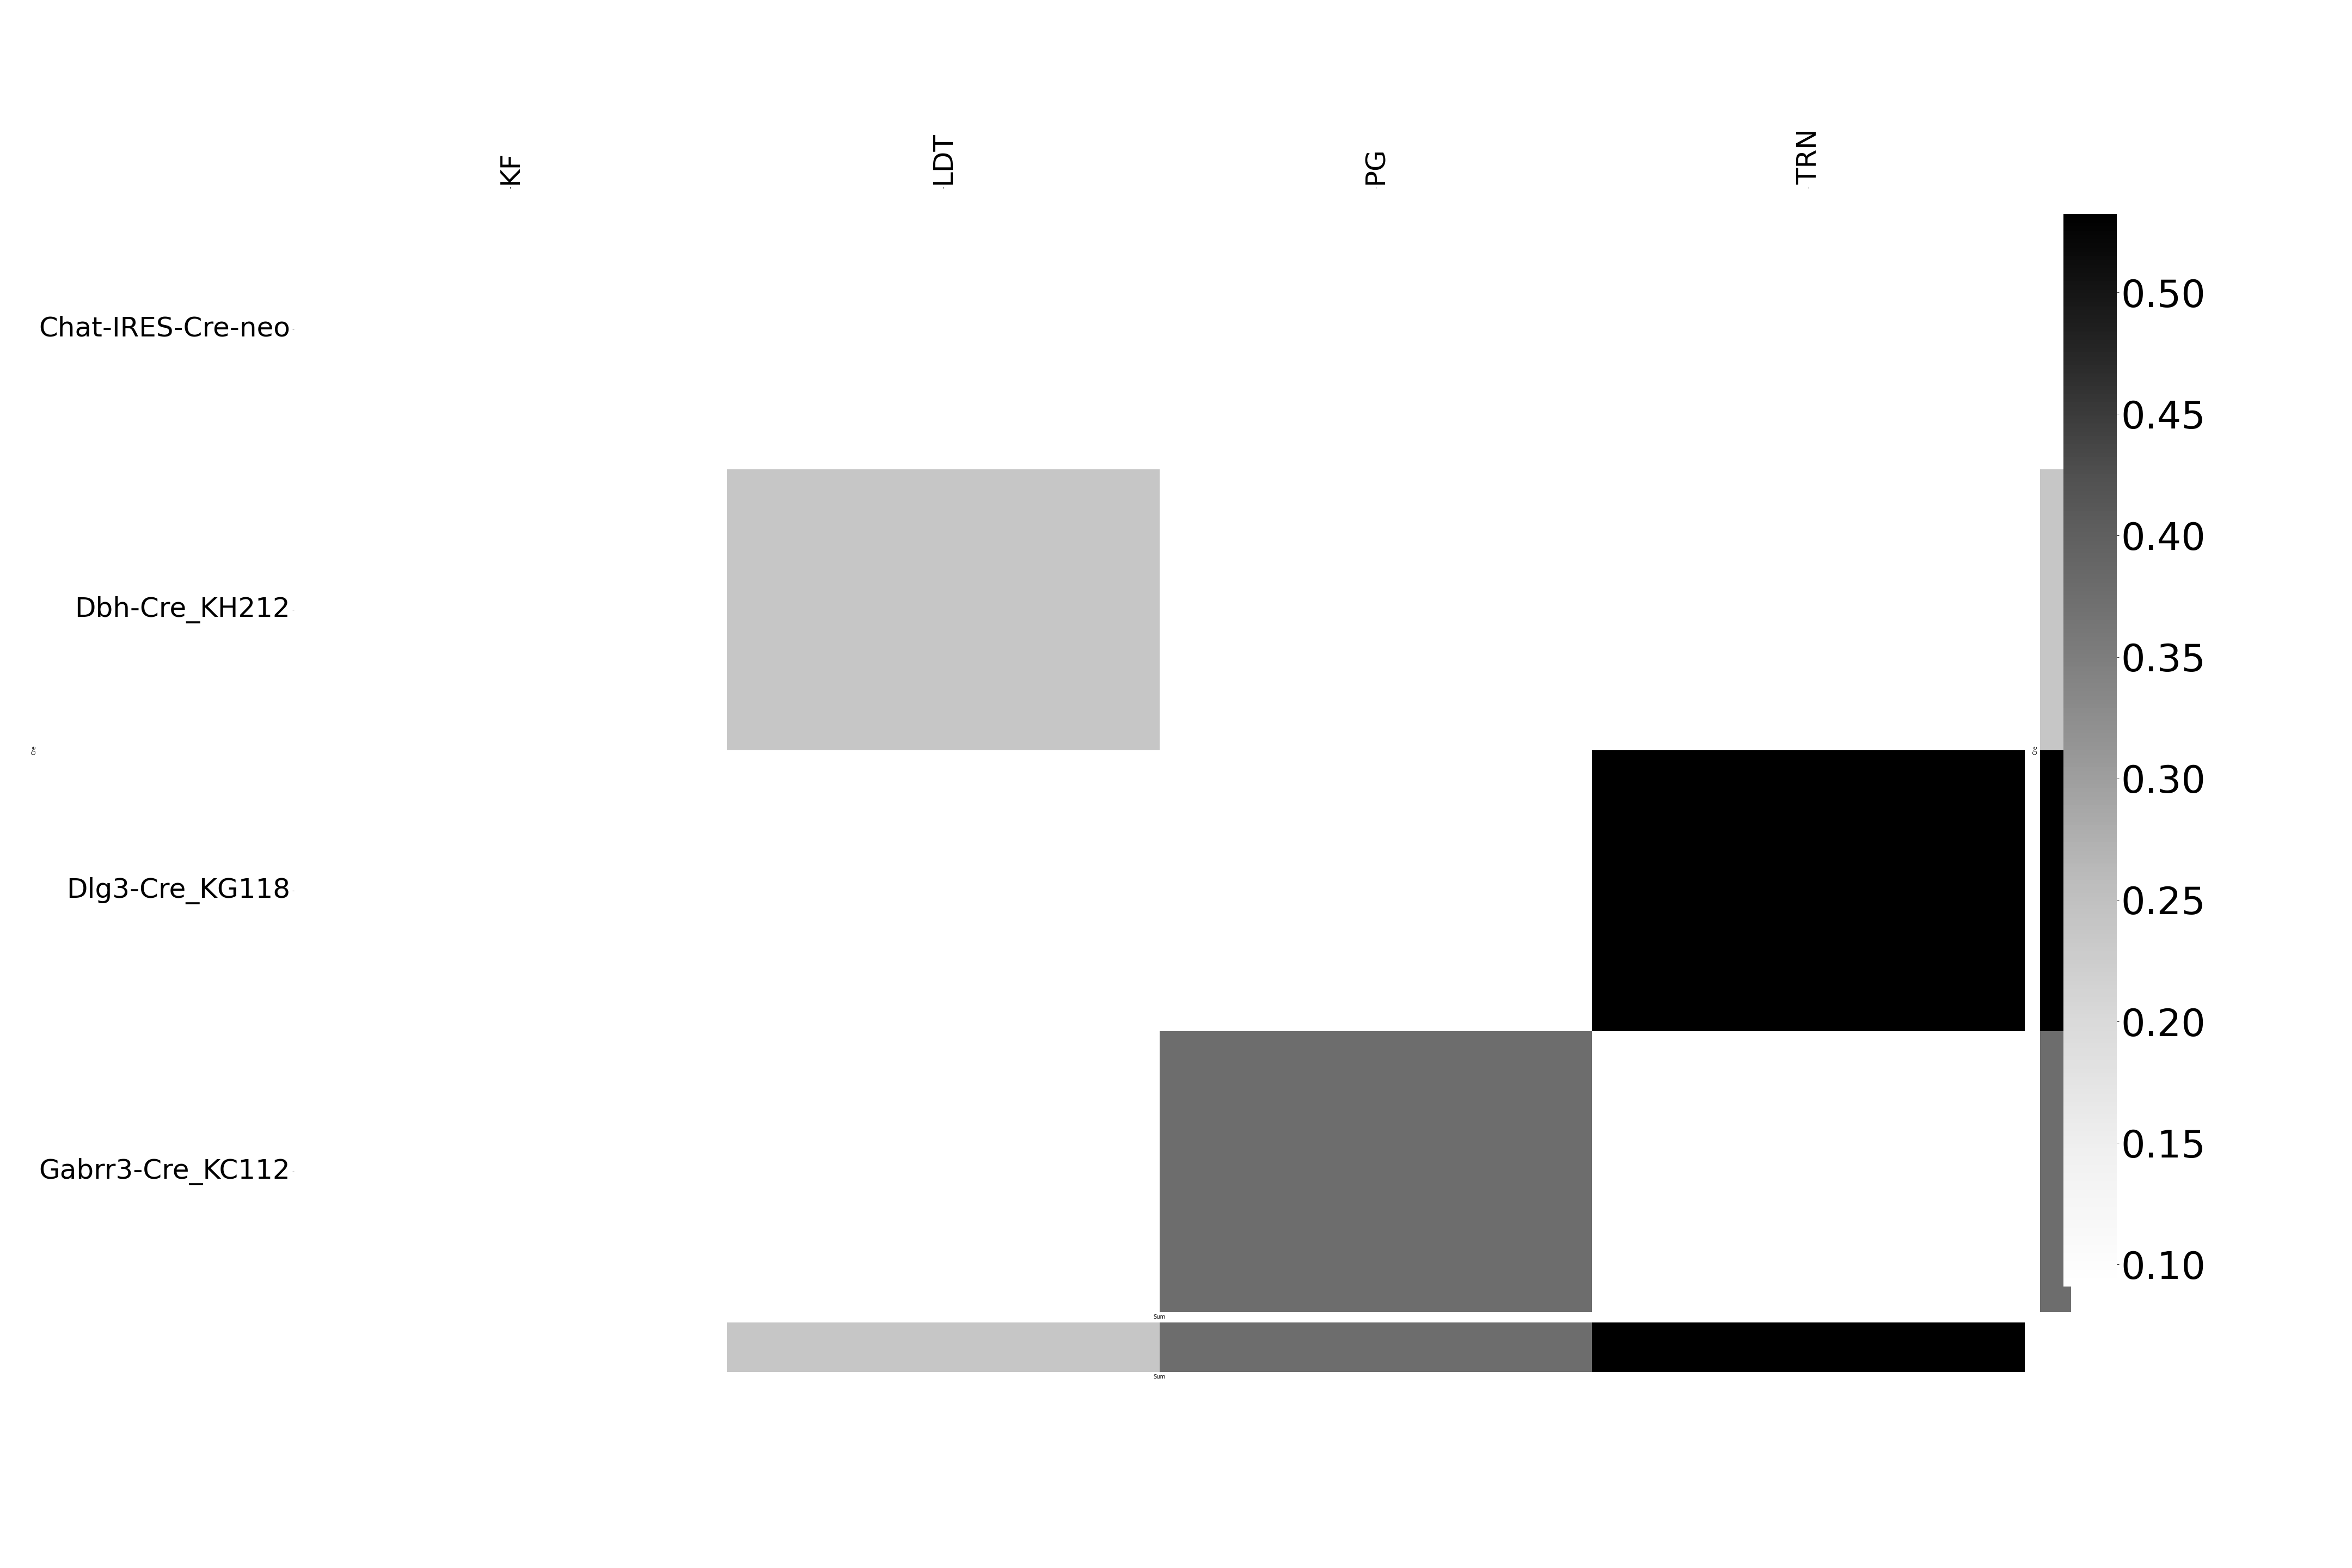
\includegraphics[width = 7in]{figs/lossdetails_771.png} 
    \label{fig:distances}
    \caption{Weighted loss for cre-leaf combinations in P. Missing values are omitted.    Row and column averages are also plotted.}
\end{figure}
\begin{figure}[H]
    \centering
    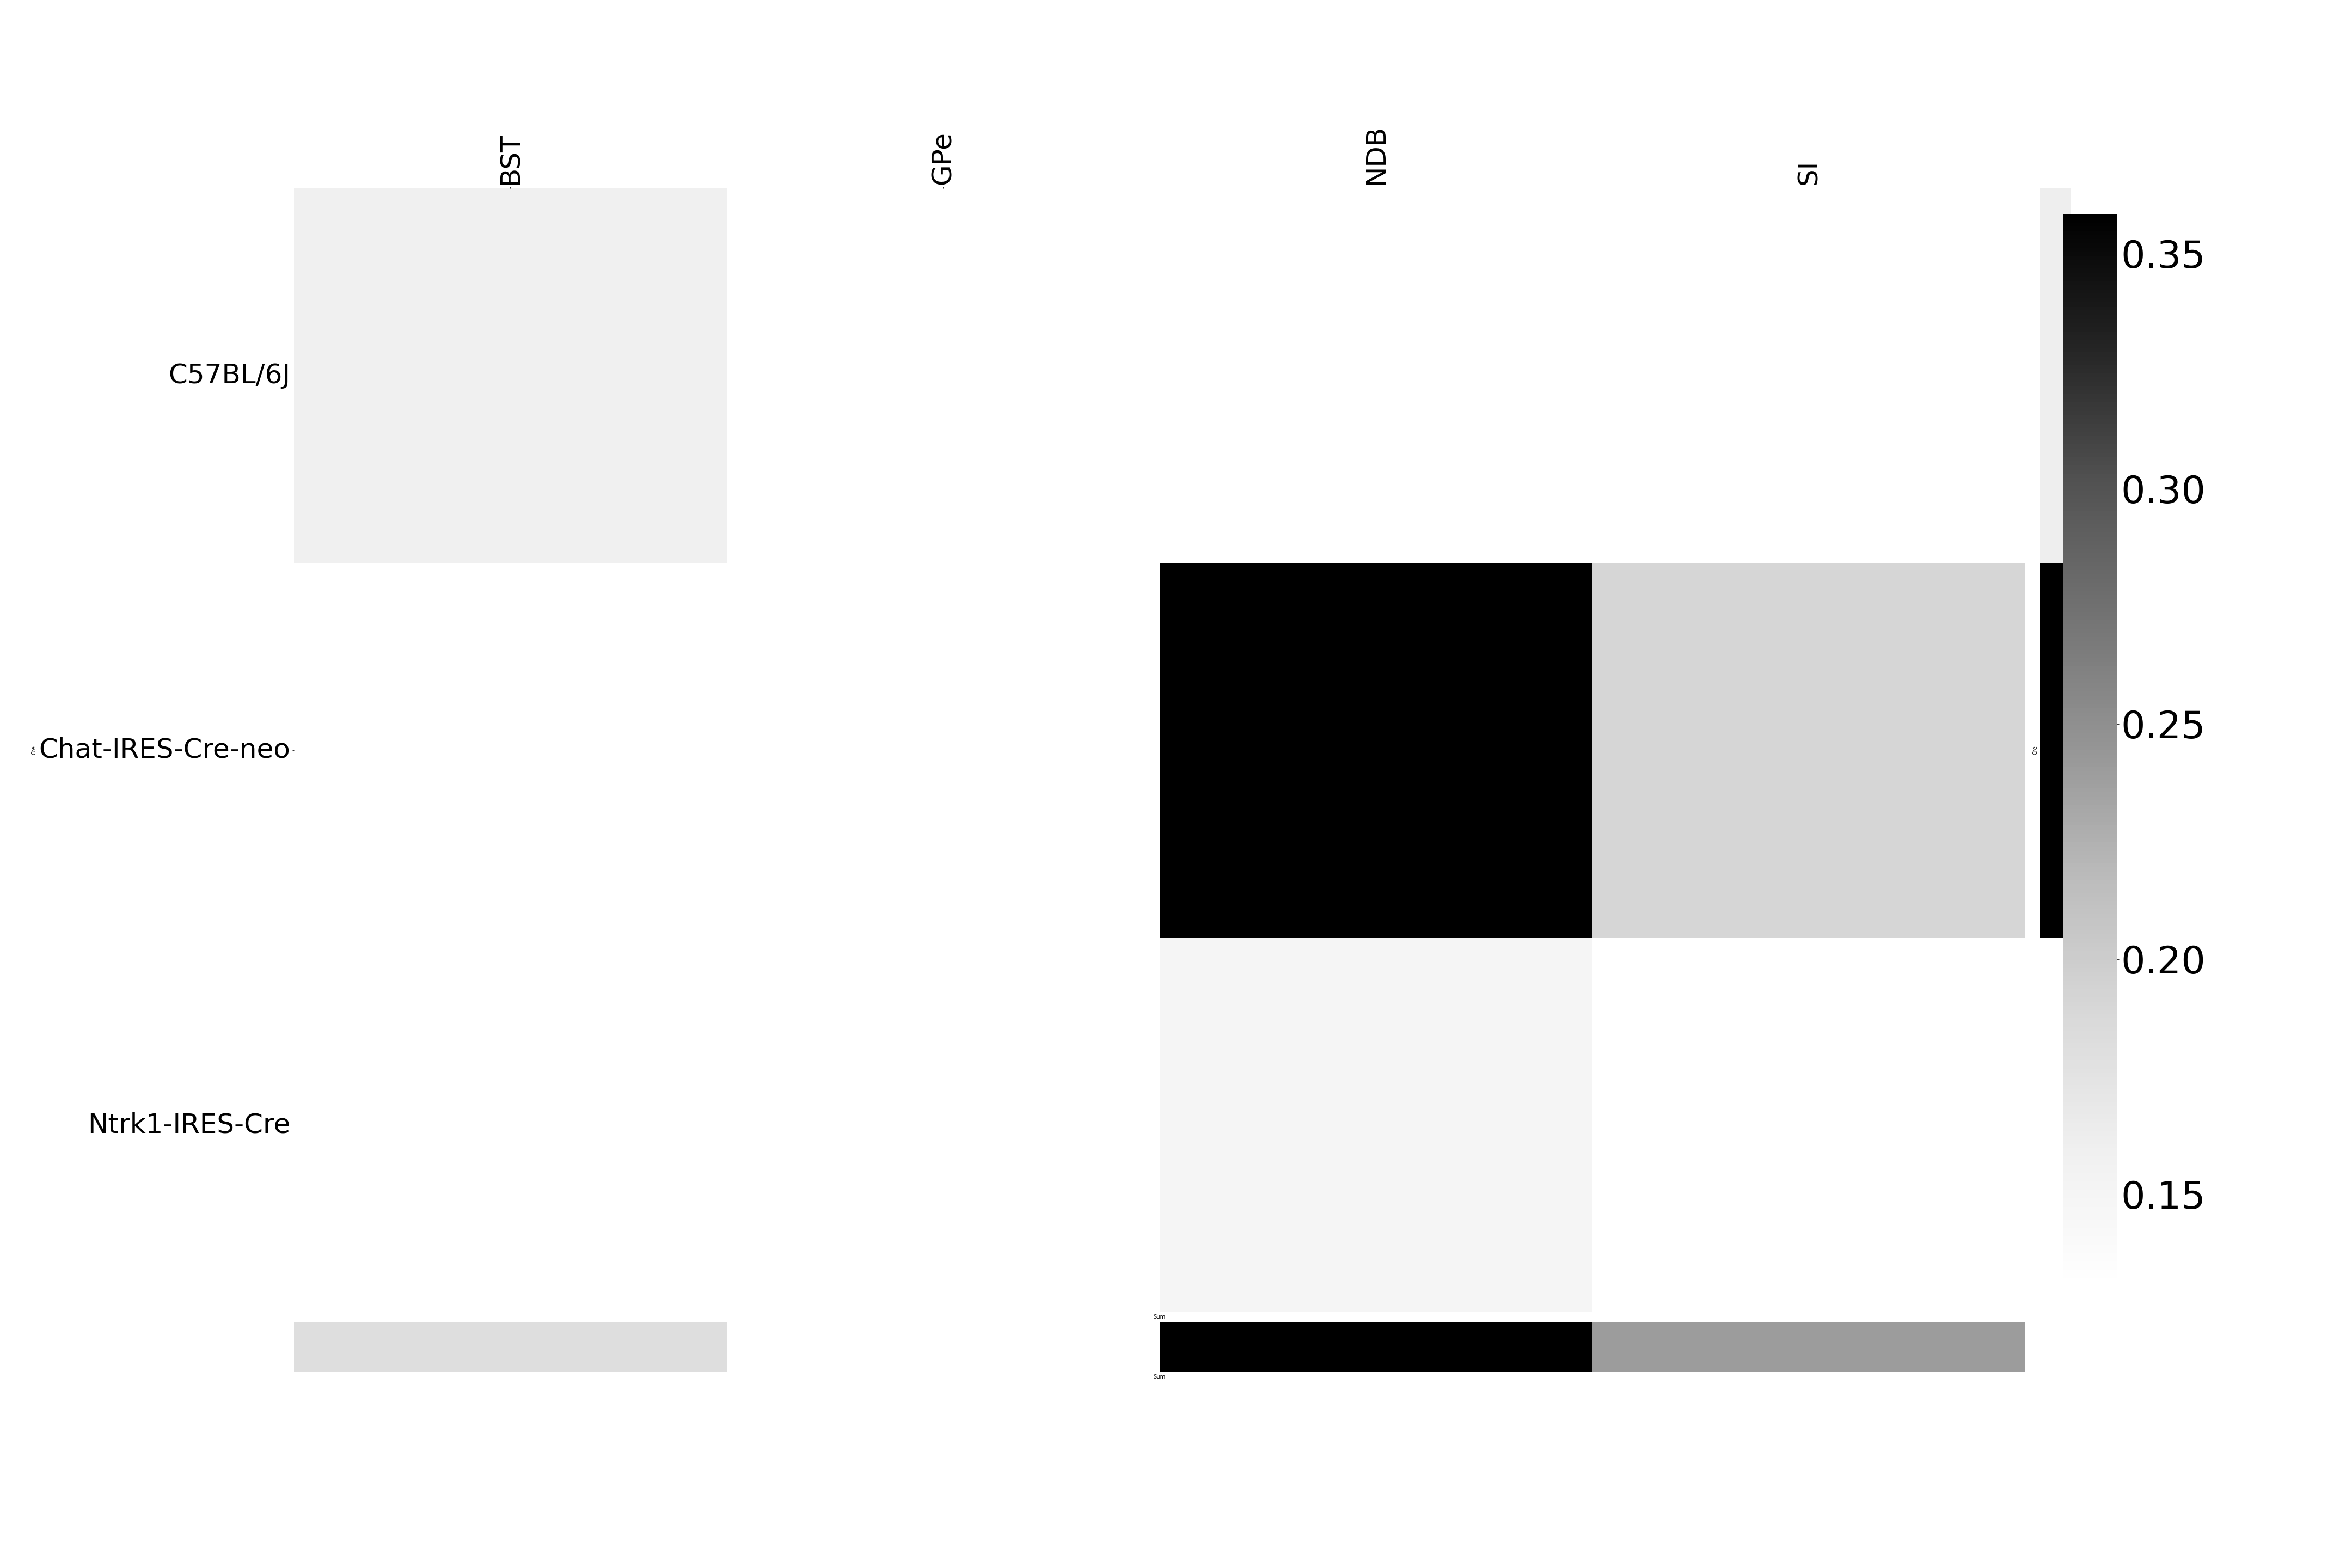
\includegraphics[width = 7in]{figs/lossdetails_803.png} 
    \label{fig:distances}
    \caption{Weighted loss for cre-leaf combinations in PAL. Missing values are omitted.  Row and column averages are also plotted.}
\end{figure}

\begin{figure}[H]
    \centering
    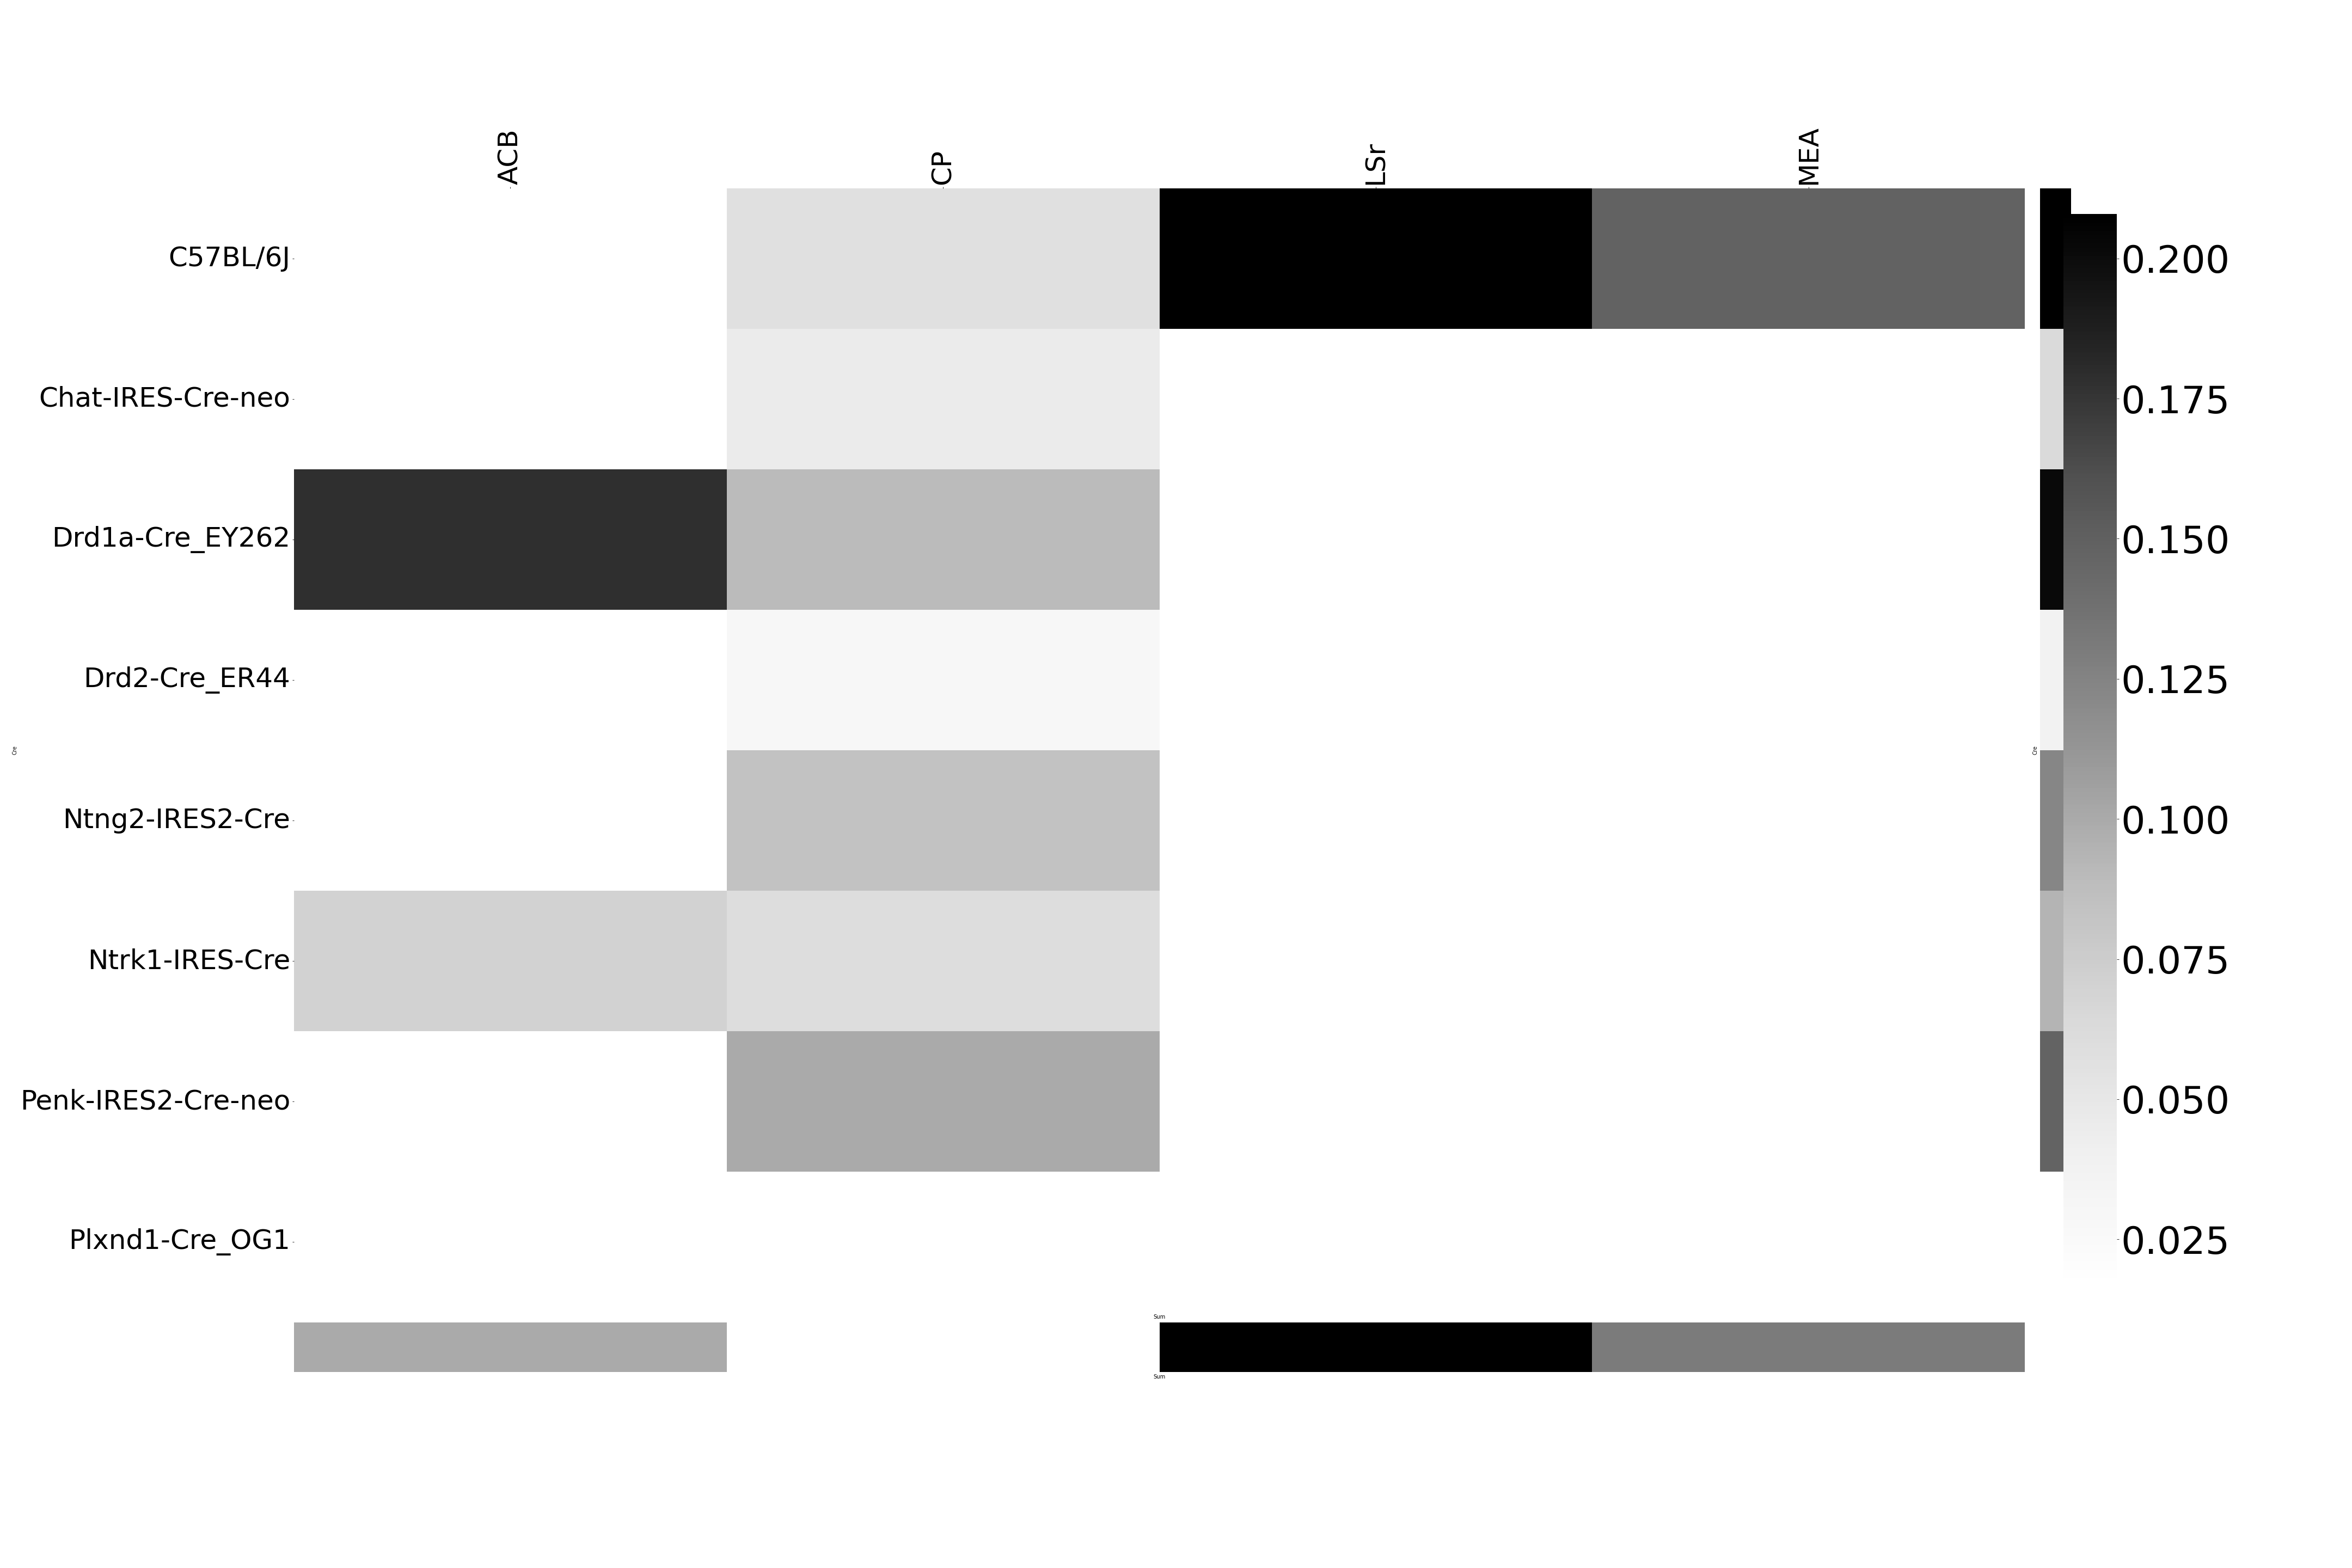
\includegraphics[width = 7in]{figs/lossdetails_477.png} 
    \label{fig:distances}
    \caption{Weighted loss for cre-leaf combinations in STR. Missing values are omitted.   Row and column averages are also plotted.}
\end{figure}

\begin{figure}[H]
    \centering
    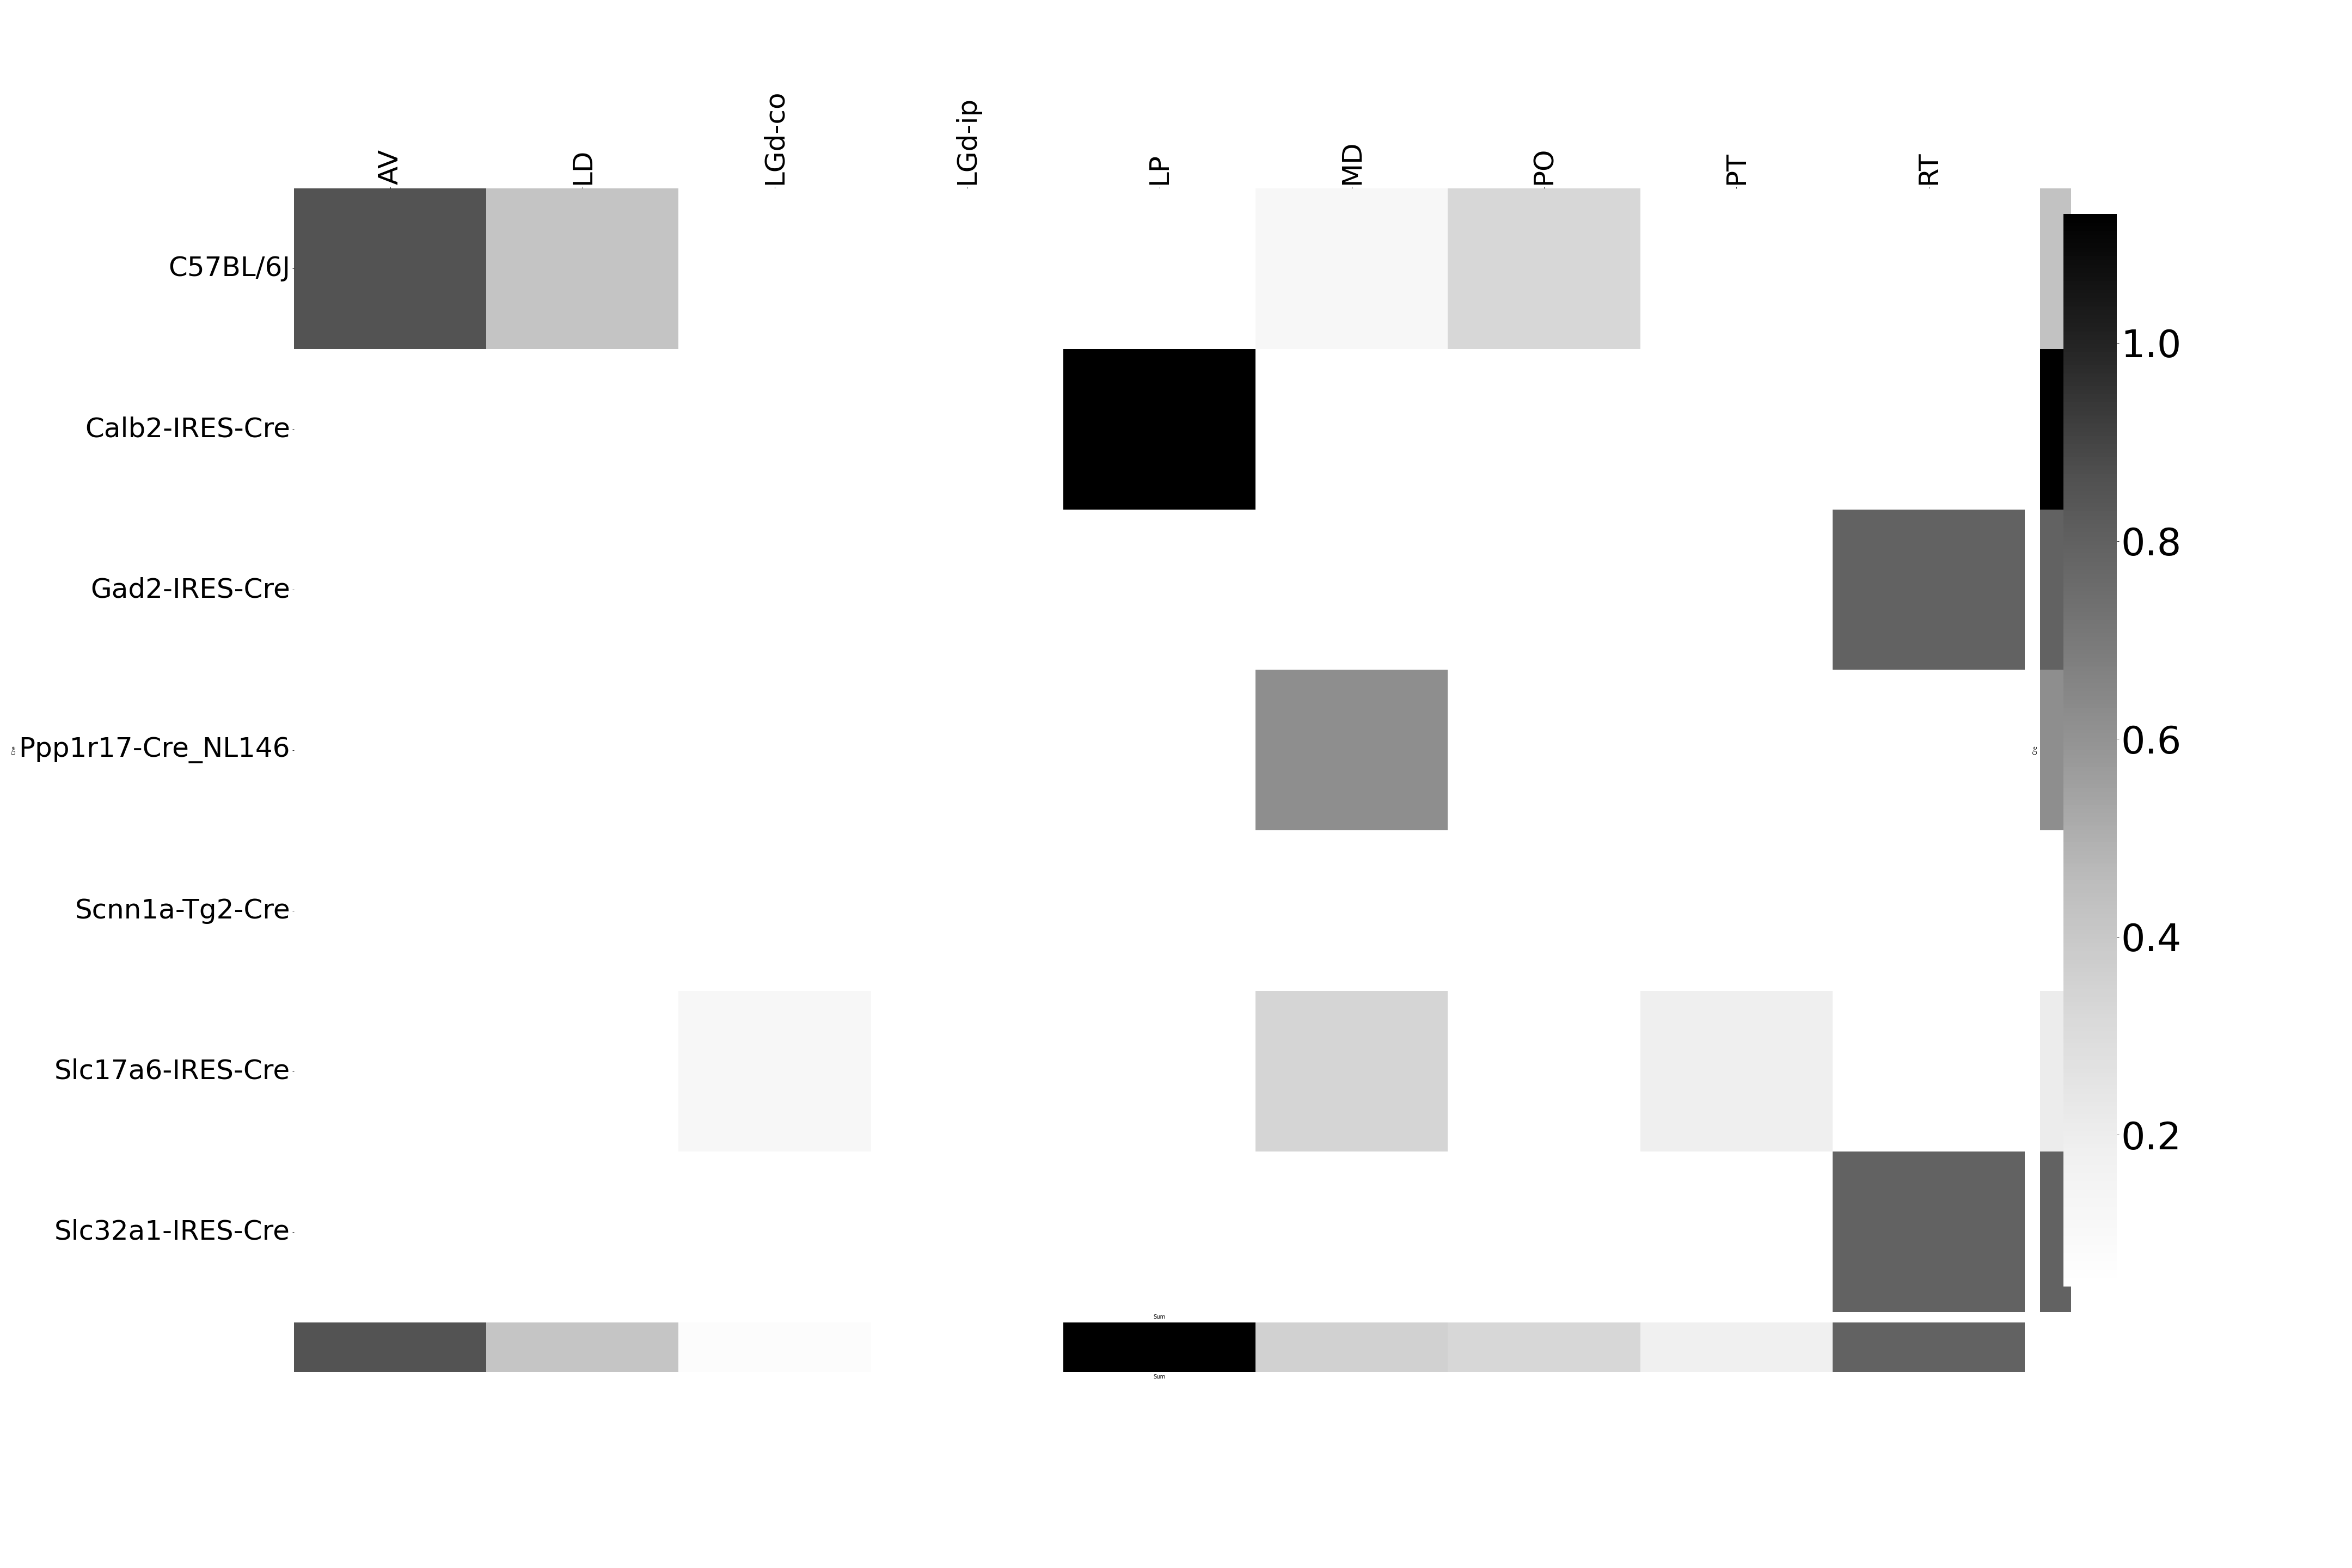
\includegraphics[width = 7in]{figs/lossdetails_549.png} 
    \label{fig:distances}
    \caption{Weighted loss for cre-leaf combinations in TH. Missing values are omitted.   Row and column averages are also plotted.}
\end{figure}

\newpage

\subsection{Matrix Factorization}
\label{supp_sec:matrix_factor_results}

We give additional results on the generation of the archetypal connectome patterns.
These consist of cross-validation selection of $q$, the number of latent components, stability analysis, and visualization of the reconstructed wild-type connectivity.

\subsubsection{Cross-validation}

We set $\alpha = 0.002$ and run Program \ref{eq:nmf} on $\mathcal C_{wt}$.
We use a random mask with $p = .3$ to evaluate prediction accuracy of models trained on the unmasked data on the masked data.
To account for stochasticity in the NMF algorithm, we run $R = 8$ replicates at each potential dimension $q$.
This selects $\hat q = 60$.

\begin{figure}[H]
    \centering
    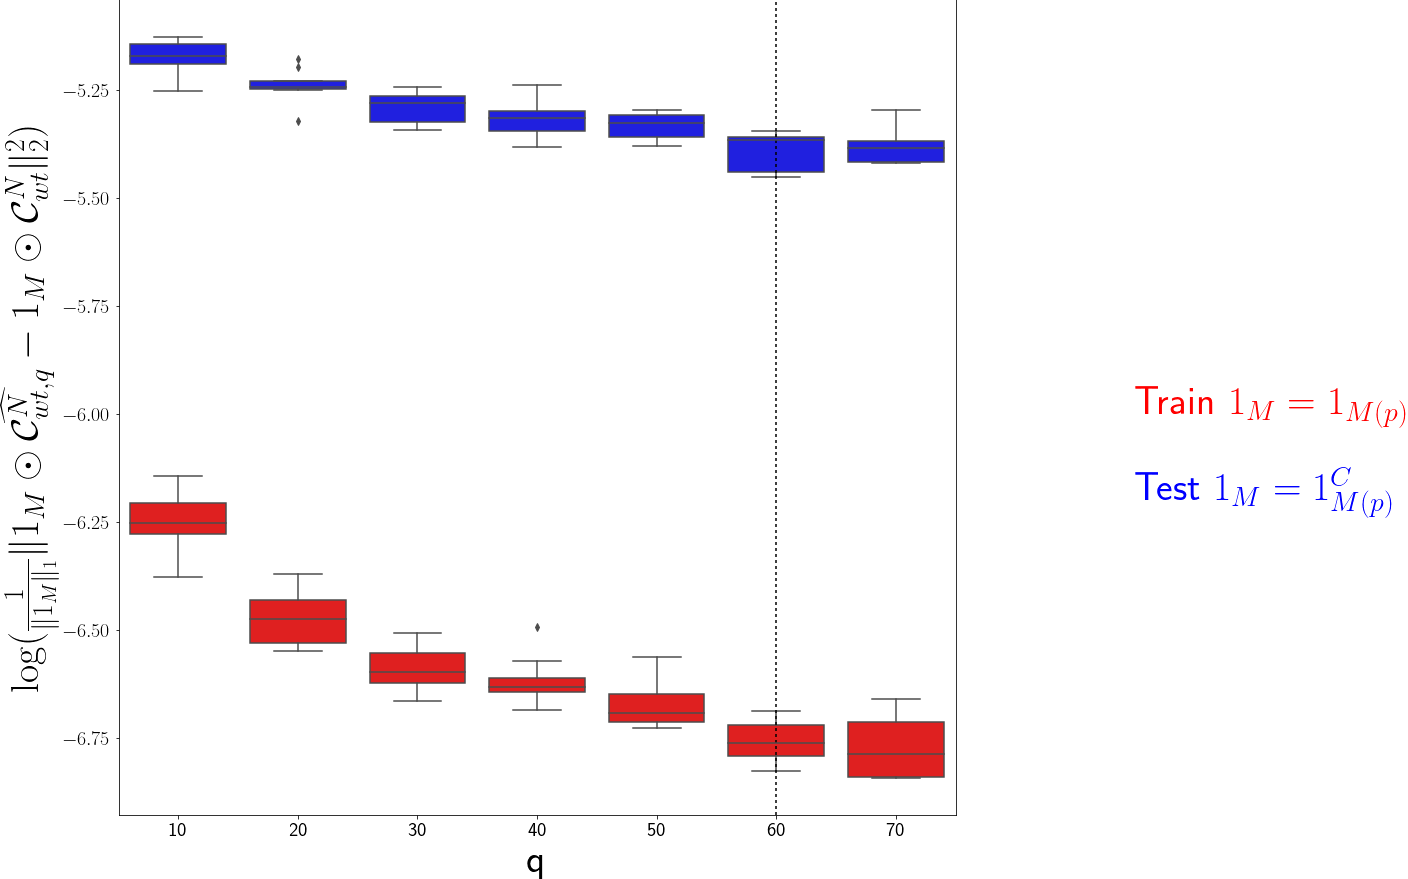
\includegraphics[width = 5in]{figs/nmf_test_train.png} 
    \label{fig:train_test}
    \caption{Train and test error using NMF decomposition.}
\end{figure}

\newpage

\subsubsection{Stability}

For the purposes of visualization and interpretability, we restrict to a $q = 15$ component model.
To address the instability of the NMF algorithm in identifying components, we $k-means$ cluster components over $R = 10$ replicates with $k \in \{10,15,20, 25, 30\}$.
Since the clustering is itself unstable, we repeat the clustering $25$ times and select the $k$ with the largest Rand index.

\begin{tabular}{lrrrrr}
\toprule
%{} &          0 &          1 &          2 &          3 &          4 \\
%\midrule
q          &  10.000000 &  20.000000 &  30.000000 &  40.000000 &  50.000000 \\
Rand index &   0.772544 &   0.844981 &   \textbf{0.932957} &   0.929827 &   0.885862 \\
\bottomrule
\end{tabular}

Since $k$-means is most stable at $k=30$, we cluster the $qR = 150$ components into $30$ clusters and select the $15$ clusters appearing in the most replicates.
\begin{figure}[H]
    \centering
    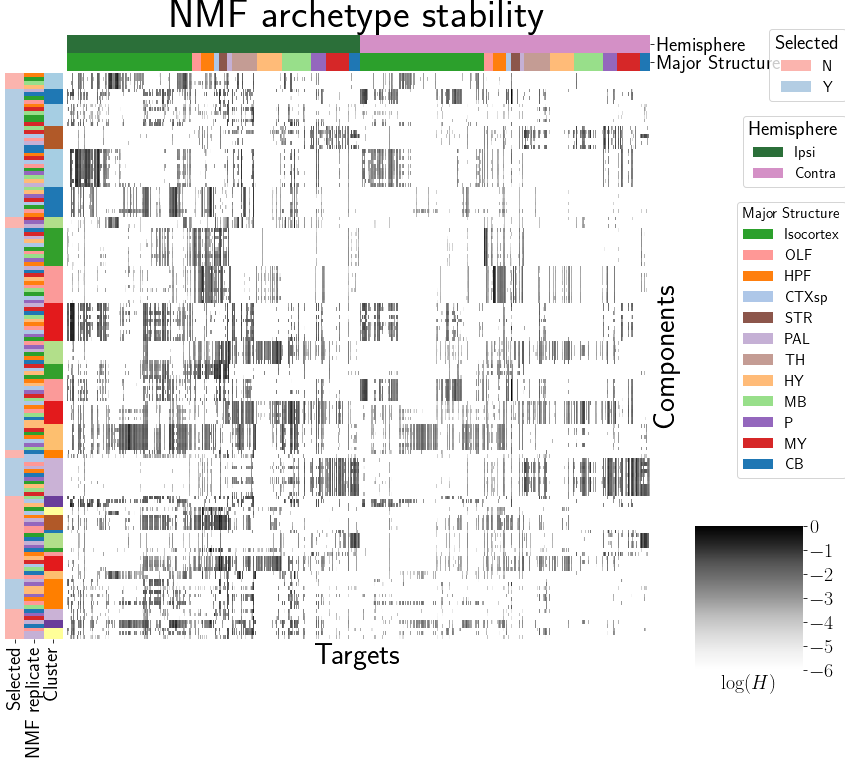
\includegraphics[width = 5in]{figs/nmfcluster.png} 
    \label{fig:distances}
    \caption{Stability of NMF results across replicates. 
    Replicate and NMF component are shown on rows.
    Components that are in the top $15$ are also indicated.}
\end{figure}
These are the components whose medians are plotted in Figure \ref{fig:H}.

\newpage

%A good $f$ will have low error on the training data, and also low error on the test data, indicating that it has not overfit.
%Although there is no assumed dichotomy between $X$ and $Y$ in unsupervised learning, for techniques like autoencoders, the above paradigm still applies, i.e., one can still hold out values of $X$.

%http://alexhwilliams.info/itsneuronalblog/2018/02/26/crossval/


